\documentclass[12pt,leqno]{book}
\newcommand{\theyear}{2020}
\newcommand{\theterm}{Winter }
\newif\ifproblemsA


%\usepackage[polutonikogreek,english]{babel}

%\usepackage{dingbat}
\usepackage{amsfonts}
\usepackage{amsmath}
\usepackage{amssymb}
\usepackage{amsthm}
\usepackage{textcomp}
\usepackage[margin=1in, paperwidth=8.5in, paperheight=11in]{geometry}
%\usepackage{ahmacros}
\usepackage{tikz}
\usetikzlibrary{calc}
\usetikzlibrary{intersections}
\usetikzlibrary{decorations.pathmorphing}
\usetikzlibrary{decorations.pathreplacing}
\usetikzlibrary{shapes.geometric}
\usetikzlibrary{fadings}
\usepackage{array}
\usepackage{multicol}
\usepackage{longtable}
\usepackage{array}
\usepackage{ragged2e}
\usepackage[pdfpagelabels]{hyperref}                 % For creating hyperlinks in cross references
\usepackage{calc}
\usepackage{fullpage}
%\usepackage{enumerate}
\usepackage{graphicx}
\usepackage{makeidx}
\usepackage{wrapfig}
%\usepackage{geometry}                % See geometry.pdf to learn the layout options. There are lots.
%\geometry{letterpaper}                   % ... or a4paper or a5paper or ... 
\usepackage{fancyhdr}

\usepackage{enumitem}

\pagestyle{fancy}
\setlength{\headheight}{30pt}


%\parindent 1cm
%\parskip 0.2cm
%\topmargin 0.2cm
%\oddsidemargin 1cm
%\evensidemargin 0.5cm
%\textwidth 15cm
%\textheight 21cm
%\parindent 1cm
%\parskip 0.2cm
%\topmargin -0.25in
%\headheight 0.25in
%\headsep 0.25in
%\oddsidemargin 0.5in
%\evensidemargin 0in
%\textwidth 6in
%\textheight 8.5in
\newtheorem{theorem}{Theorem}[section]
\newtheorem{proposition}[theorem]{Proposition}
\newtheorem{corollary}[theorem]{Corollary}
\newtheorem{lemma}[theorem]{Lemma}
\newtheorem{remark}[theorem]{Remark}
\newtheorem{definition}[theorem]{Definition}

\newcommand{\defnstyle}{\emph}
%\newcommand{Venumerate}{enumerate}
%\newenvironment{Venumerate}{\begin{enumerate}}{\end{enumerate}}
\newcommand{\rec}[1]{\frac{1}{#1}}


\newif\ifsolns
\newif\ifmathlab


\newcommand{\soln}{\textbf{ANSWER: }}

\newenvironment{alphenumerate}%
   {\begin{enumerate}%
      \renewcommand{\theenumi}{\alph{enumi}}%
      \renewcommand{\labelenumi}{(\theenumi)}}
   {\end{enumerate}}





\def\textdefn{\textbf{Definition:~}}

% \cleartoevenpage acts like \newpage, but guarantees that you'll be at the start of a two-page spread.
\newcommand*\cleartoevenpage{%
  \clearpage%
  \ifodd\value{page}\thispagestyle{empty}\begin{center}\em This page intentionally left blank.\end{center}\clearpage\fi}

\newcommand*\cleartooddpage{%
  \clearpage%
  \ifodd\value{page} \else\thispagestyle{empty}\begin{center}\em This page intentionally left blank.\end{center}\clearpage\fi}


\newlength\boxedblankwidth
\setlength{\boxedblankwidth}{.98\textwidth}
\advance\boxedblankwidth by -\leftmargin
\newcommand\boxedblank[2][1in]{\fbox{\raisebox{0pt}[\height][#1]{\parbox[t]{\boxedblankwidth}{#2}}}}

\newlength\textwidthinlist
\newcommand\computetextwidthinlist{\textwidthinlist=\textwidth
                                   \advance\textwidthinlist by -\leftmargin
                                   \advance\textwidthinlist by -\rightmargin}

%\HOMEWORK creates the heading for the homework section, including a \newpage command and an entry in the table of contents.
%\HOMEWORK* creates the same heading and TOC entry, but no \newpage command.
%\HOMEWORK** merely typesets the heading, but does not force a \newpage and does not put anything in the table of contents.
%            This is good for a section containing nothing but the homework questions.
\newcounter{hwkno}
\setcounter{hwkno}{1}

\makeatletter
  \newcommand{\HOMEWORK}{\@ifstar\HOMEWORKatleastonestar\HOMEWORKnostar}
  \newcommand{\HOMEWORKnostar}{%
  \cleartooddpage \pagestyle{hwk}
	\ifmathlab \solnsfalse \fi
%  	\cleardoublepage
%    \newpage
    \HOMEWORKheading \stepcounter{hwkno} 
    \HOMEWORKcontentsline}
  \def\HOMEWORKatleastonestar{\HOMEWORKcheckforsecondstar}
  \newcommand{\HOMEWORKcheckforsecondstar}{\@ifstar\HOMEWORKdoublestar\HOMEWORKsinglestar}
  \newcommand{\HOMEWORKsinglestar}{%
    \HOMEWORKheading
    \HOMEWORKcontentsline}
  \newcommand{\HOMEWORKdoublestar}[1]{%
    \HOMEWORKheading}
  \def\HOMEWORKheading{\subsubsection*{Homework \thehwkno}}
  \def\HOMEWORKcontentsline{\addcontentsline{toc}{subsubsection}{Homework}}
\makeatother

\newcommand{\ENDHOMEWORK}{\cleartooddpage  \ifmathlab \solnstrue \fi \pagestyle{normal}}

\def\pageover{%
  \ifodd\value{page}%
    \par\rule{0pt}{0pt}\hfill\emph{(over)}%
  \fi}

\def\solnsnewpage{}
\def\perspectiveHWnewpage{}

% Use \hwnewpage in the homework sections instead of \newpage.
% This guarantees that if you're at the bottom of an odd (right-hand) page,
% the word "(over)" will appear to remind students there's more homework on the next page.
\def\hwnewpage{%
  \pageover
  \newpage
}







\newcounter{currentyear}
\setcounter{currentyear}{\theyear}
\newcounter{tempyear}


\makeatletter
\let\xa=\expandafter
\newcommand\declareproblemlettering[1]{%
  \newcounter{#1@enum}%
  \setcounter{#1@enum}{0}%
  \newenvironment{#1enumerate}%
    {\begin{list}{\stepcounter{#1@enum}%
                  #1\arabic{#1@enum}.%
                  \xdef\@currentlabel{#1\arabic{#1@enum}}%
                  \gdef\p@enumii{#1\arabic{#1@enum}}%
                  %\gdef\labelenumii{(\theenumii)}%
                  \gdef\theenumii{(\alph{enumii})}%
                  \gdef\labelenumii{\theenumii}%
                  }{}
     \@enumdepth=1}%
    {\end{list}}%
}

\newcounter{numstudentsolns}
\setcounter{numstudentsolns}{0}

\newcommand\studentsoln[1]{%
  %Saves the parameter as a student solution
  \stepcounter{numstudentsolns}%
  %\showthe\c@numstudentsolns
  \xa\xdef\csname studentsoln-label-\roman{numstudentsolns}\endcsname{\@currentlabel}%
  %\xa\show\csname studentsoln-label-\roman{numstudentsolns}\endcsname%
  \xa\long\xa\gdef\csname studentsoln-\roman{numstudentsolns}\endcsname{#1}%
  %\xa\show\csname studentsoln-\roman{numstudentsolns}\endcsname%
}

\newcommand\saveasstudentsoln[1]{%
  \studentsoln{#1}%
  #1%
}

\newcommand\gradersoln[1]{%
  %Gives text that shows up for graders' manual only.
  \ifsolns
    #1%
  \fi
}



\newcommand\solution{%
  \@ifnextchar*\soln@star\soln@nostar%
}
\long\def\soln@star*#1{%
  \studentsoln{#1}%
  \gradersoln{\par\soln #1}%
}
\long\def\soln@nostar#1{%
  \gradersoln{\par\soln #1}%
}

\newcommand\esolution{%
  \@ifnextchar*\esoln@star\esoln@nostar%
}
\long\def\esoln@star*#1{%
  \edef\temp@soln{#1}%
  \xa\soln@star\xa*\xa{\temp@soln}%
}
\long\def\esoln@nostar#1{%
  \edef\temp@soln{#1}%
  \xa\soln@nostar\xa{\temp@soln}%
}

\newif\ifstudentsolns
\newif\ifgradersolns

\newcommand\studentsolnscale[1][0.5]{%
  \ifstudentsolns
    \tikzset{scale=#1}
  \fi
}
\newcommand\sspar{%
  \ifstudentsolns
    ~\par
  \fi
}



\newcounter{numattributions}
\setcounter{numattributions}{0}

\newcommand\saveattribution[1]{%
  %Saves the parameter to be displayed in the attributions section
  \stepcounter{numattributions}%
  \edef\attributionlabelname{attribution@page@\roman{numattributions}}
  \xa\label\xa{\attributionlabelname}
  \xa\long\xa\gdef\csname attribution-\roman{numattributions}\endcsname{#1}%
}


\makeatother


%--------------------------------------------------------------------
\makeatletter
%                            \fillwithlines


% \fillwithlines takes one argument, which is either a length or \fill
% or \stretch{number}, and it fills that much vertical space with
% horizontal lines that run the length of the current line.  That is,
% they extend from the current left margin (which depends on whether
% we're in a question, part, subpart, or subsubpart) to the right
% margin.
%
% The distance between the lines is \linefillheight, whose default value
% is set with the command
%
% \setlength\linefillheight{.25in}
%
% This value can be changed by giving a new \setlength command.
%
% The thickness of the lines is \linefillthickness, whose default value
% is set with the command
%
% \setlength\linefillthickness{.1pt}
%
% This value can be changed by giving a new \setlength command.


\newlength\linefillheight
\newlength\linefillthickness
\setlength\linefillheight{.25in}
\setlength\linefillthickness{0.1pt}

\newcommand\linefill{\leavevmode
    \leaders\hrule height \linefillthickness \hfill\kern\z@}


\def\fillwithlines#1{%
  \begingroup
  \ifhmode
    \par
  \fi
  \hrule height \z@
  \nobreak
  \setbox0=\hbox to \hsize{\hskip \@totalleftmargin
          \vrule height \linefillheight depth \z@ width \z@
          \linefill}%
  % We use \cleaders (rather than \leaders) so that a given
  % vertical space will always produce the same number of lines
  % no matter where on the page it happens to start:
  \cleaders \copy0 \vskip #1 \hbox{}%
  \endgroup
}
\makeatother
%--------------------------------------------------------------------

\newcounter{lettercount}
\newcounter{numbercount}
\setcounter{lettercount}{1}
\setcounter{numbercount}{1}

\newcommand{\vletter}{\Alph{lettercount}. \stepcounter{lettercount}&}
\newcommand{\vnumber}{\arabic{numbercount}. \stepcounter{numbercount}&}

%--------------------------------------------------------------------
\usepackage{tikz}
\usepackage{pgfplots}
\pgfplotsset{compat=1.12}

 
\ifmathlab \solnstrue \fi
%\mathlabtrue
%\solnstrue
%\problemsAtrue

\makeindex

\title{MA 106: \\ Mathematics of Democracy }

\author{Anders O.F. Hendrickson \qquad
        St.~Norbert College  \\
        Mariah Birgen \qquad
				Wartburg College}

\date{\theterm{} \theyear}
\lhead{Mathematics of Democracy}
\lfoot{Mariah Birgen} \rhead{\rightmark}
\lhead{\leftmark}\cfoot{\thepage} \rfoot{\theterm \theyear}


% Define the (unnumbered) title page layout here
\newcommand{\mytitlepage}{
	\pagenumbering{alph}
	\thispagestyle{empty}
	\beforepartskip
	\begin{center}
	\thetitle

	\theauthor
	\end{center}
	\afterpartskip
	\clearpage
}

%Normal Page Style
\fancypagestyle{normal}{ %
	\fancyhf{} % remove everything
		\lhead{Mathematics of Democracy}
		\lfoot{Mariah Birgen} \rhead{\rightmark}
		\lhead{\leftmark}\cfoot{\thepage} \rfoot{\theterm{}\, \theyear}
	}
	
	%HOMEWORK header - 
\fancypagestyle{hwk}{ %
   \fancyhf{} \lfoot{Mariah Birgen} \cfoot{\rightmark}
 \rfoot{\theterm{}\, \theyear} \rhead{Name: \underline{\hspace{2.5in}}}

 % remove everything
  %\renewcommand{\headrulewidth}{0pt} % remove lines as well
  %\renewcommand{\footrulewidth}{0pt}
}

%\includeonly{
%options,
%chapter-Redistricting
%}

\begin{document}

\frontmatter
%\thispagestyle{empty}
	%\pagenumbering{alph}
	\thispagestyle{empty}
	%\beforepartskip
	\vfill
	\maketitle
	%\begin{center} \Large
	%\thetitle
%
	%\theauthor
	%\end{center}
	%%\afterpartskip
	\vfill
	\clearpage

\pagestyle{empty}
~\clearpage

 \addcontentsline{toc}{chapter}{Contents}
	%\pagenumbering{alph}
		\thispagestyle{empty}
\tableofcontents*
%\listoffigures
%\listoftables


\chapter*{Preface}\normalsize
%\renewcommand{\thepage}{\arabic{page}}% Arabic numerals for page counter

%\pagenumbering{roman}
  \addcontentsline{toc}{chapter}{Preface}
  \markboth{PREFACE}{} %Sets the headings, so it doesn't still say "CONTENTS"
This is not a textbook.
You will find in these printed pages almost no formulae, answers, or information.
This book will not tell you how to do anything.
So what is this book?
It is most emphatically a \emph{workbook}: a place to work on learning mathematics by doing it yourself.

The mathematics in this book will, for the most part, be content that you have never seen or thought about before.  However, it is material that you can figure out with some patience and persistence.  The point to keep in mind is that you are not expected to know beforehand.  To learn the content, use the following devices:
\begin{itemize}
	\item Try something.
	\item Ask yourself why what you have tried doesn't work.
	\item Brainstorm by yourself.
	\item Brainstorm with your neighbors or your team members.
	\item Be willing to say what you are thinking and ask questions.
	\item Be willing to challenge the statements of others (including the teacher).
\end{itemize}

One of the most important skills in life, a skill highly valued by employers and spouses alike,
is the ability to solve problems no one has taught you how to do.
Any monkey or computer can be taught to follow a rote procedure over and over again,
and frankly, your previous math courses probably treated you like a monkey.
It is when you
  \begin{itemize}
		\item encounter unforeseen difficulties,
		\item swiftly learn from experience,
		\item and devise a suitable plan to overcome them
	\end{itemize}
that you show yourself to have a human mind.
One of the chief goals of MA 106
is for you to practice this highly creative, utterly vital, and most fully human act
of doing what you can't do.

There are places in this book for taking notes, and in particular for noting the meanings of mathematical terms. It has become clear over the past five years that the physical act of writing down notes by hand using a pencil or paper leads to significantly superior learning over recording audio or taking pictures with your camera.
Please don't restrict your note-taking to just filling in the blanks, though!
There will often be essential points covered in class
that do not have a corresponding blank space in these pages.
It's up to you whether to take your other notes in the margins of this workbook or in another notebook,
but you should take them just as assiduously in this course as in any other course.
%This advice is particularly important for chapters \ref{ch:finance} and \ref{ch:perspective}.

There are places in this book where we assume that you have a calculator to do things for you.  You will need a calculator that will put any number into an exponent, so look for a button that is labeled $\wedge$ or $x^y$.  You will need a calculator that will calculate standard deviations for you, so make sure that the calculator has the ability to perform statistical calculations.

There will be a lot of trial and error as you work in these pages,
so I recommend using a pencil rather than a pen!

%\newpage
%\pagestyle{fancy}
~\ifodd\value{page}\relax\else\newpage\fi

%\pagestyle{headings}

\mainmatter

\pagestyle{fancy}
%\pagenumbering{arabic}
%chapter-Voting.tex

%<*CHAPTERHEADER>

\declareproblemlettering{V}
\pagestyle{fancy}
\cleartooddpage


\chapter{Voting Theory}\label{ch:votingtheory}

%</CHAPTERHEADER>

%<*WORKSHEETS>
\section{Voting Systems}


\begin{enumerate}
  \item The Bellevue Taxicab Union is preparing to elect its president. 
        Three members are considering running for president:  Alice, Bob, and Charles.
        Each of the five voters has a first, second, and third choice,
        as listed in the following table:       
           \def\A{Alice}
           \def\B{Bob}
           \def\C{Charles}
        \begin{center}
          \begin{tabular}{l||l|l|l|l|l}
            Voter: & Voter 1 & Voter 2 & Voter 3 & Voter 4 & Voter 5 \\ \hline\hline
            1st choice: & \A & \B & \B & \C & \B \\
            2nd choice: & \C & \A & \C & \A & \A \\
            3rd choice: & \B & \C & \A & \B & \C \\
          \end{tabular}
        \end{center}
        Depending on who decides to run, the ballot the voters see in the booth will look different.
        For each of the following ballots, how many votes will each candidate receive?  Who will win?
        
        \begin{center}
          \begin{tabular}{p{2.5in}p{3in}}
                  (a)
                  \begin{tabular}{|cl|}\hline
                    \multicolumn{2}{|c|}{Who should be} \\
                    \multicolumn{2}{|c|}{president?} \\ \hline
                    $\square$ & Alice  \\
                    $\square$ & Bob     \\
                    $\square$ & Charles \\
                    \hline
                  \end{tabular}
                  \ifsolns
                    \soln Bob
                  \fi
            &
                  (c)
                  \begin{tabular}{|cl|}\hline
                    \multicolumn{2}{|c|}{Who should be} \\
                    \multicolumn{2}{|c|}{president?} \\ \hline
                    $\square$ & Alice  \\
                    $\square$ & Charles \\
                    \hline
                  \end{tabular}
                  \ifsolns
                    \soln Alice
                  \fi
            \\
          \phantom{X} & \\
          (b)     \begin{tabular}{|cl|}\hline
                    \multicolumn{2}{|c|}{Who should be} \\
                    \multicolumn{2}{|c|}{president?} \\ \hline
                    $\square$ & Alice  \\
                    $\square$ & Bob     \\
                    \hline
                  \end{tabular}
                  \ifsolns
                    \soln Alice
                  \fi
            &
          (d)     \begin{tabular}{|cl|}\hline
                    \multicolumn{2}{|c|}{Who should be} \\
                    \multicolumn{2}{|c|}{president?} \\ \hline
                    $\square$ & Bob     \\
                    $\square$ & Charles \\
                    \hline
                  \end{tabular}
                  \ifsolns
                    \soln Bob
                  \fi
          \end{tabular}
        \end{center}


%\clearpage
%%%%%%%%%%%
%%%%%%%%%%%Insert instructions on how to make a preference table here!
%%%%%%%%%%%
\clearpage
   %good for Borda count
   \def\gardenmatrix{%
	\large
        \begin{center}
          \begin{tabular}{|c|c|c|c|c|c|c|c} \hline
                       & \multicolumn{5}{c|}{Number of Ballots} \\
            Ranking    &  &  &  &  &      \\ \hline\hline
            1st choice & D & D & E & F & G     \\
            2nd choice & G & G & G & G & E     \\
            3rd choice & E & F & F & D & F     \\
            4th choice & F & E & D & E & D     \\ \hline
          \end{tabular}
        \end{center}}



  \item The Shell Rock Gardening Club is electing a new Master of the Greensward.
        Four candidates are running for the position: Danielle, Edgar, Frederika, and Gustav.
				
				    \item Here is the ballot:
                \begin{center}
                  \begin{tabular}{|cl|}\hline
                    \multicolumn{2}{|c|}{Who should be Master} \\
                    \multicolumn{2}{|c|}{of the Greensward?} \\ \hline
                    $\square$ & Danielle  \\
                    $\square$ & Edgar     \\
                    $\square$ & Frederika \\
                    $\square$ & Gustav    \\ \hline
                  \end{tabular}
                \end{center}
      
				
				The members cast the following ballots:
				\begin{center}
					
				\begin{tabular}{lllll}
				            Ranking     &             1st choice  &             2nd choice  &             3rd choice  &             4th choice \\\hline
Voter 1 & Danielle  & Gustav & Edgar  &  Frederika \\\hline
Voter 2 & Danielle  & Gustav &  Frederika  & Edgar \\\hline
Voter 3 & Edgar  & Gustav &  Frederika  & Danielle \\\hline
Voter 4 &  Frederika  & Gustav & Danielle  & Edgar \\\hline
Voter 5 & Gustav & Edgar      &  Frederika      & Danielle                   \\\hline
Voter 6 & Danielle  & Gustav & Edgar  &  Frederika \\\hline
Voter 7 & Danielle  & Gustav &  Frederika  & Edgar \\\hline
Voter 8 & Edgar  & Gustav &  Frederika  & Danielle \\\hline
Voter 9 &  Frederika  & Gustav & Danielle  & Edgar \\\hline
Voter 10 & Gustav & Edgar      &  Frederika      & Danielle                   \\\hline
Voter 11 & Danielle  & Gustav & Edgar  &  Frederika \\\hline
Voter 12 & Edgar  & Gustav &  Frederika  & Danielle \\\hline
Voter 13 &  Frederika  & Gustav & Danielle  & Edgar \\\hline
Voter 14 & Edgar  & Gustav &  Frederika  & Danielle\\\hline
				\end{tabular}
				
				\end{center}
        \begin{enumerate}
				\item 				Create a preference table for this election by counting the number of voters who have the same preference and putting that number above the appropriate ballot in the table.  You may use tally marks if you prefer.
				\gardenmatrix
				\ifsolns
				  \begin{tabular}{|c|c|c|c|c|c|c|c} \hline
                       & \multicolumn{5}{c|}{Number of Ballots} \\
            Ranking    & 3 &2  &4  &3  &2      \\ \hline\hline
        \end{tabular}
				\fi
\clearpage
\item    Who will be elected Master?  What percent of the vote will he or she have? \label{Ch1Prob3b}
							
                \ifsolns
                  \par\soln D, with $\frac{5}{14}\approx 35.7\%$
                \fi
								
              	\fillwithlines{\stretch{1}}
          \item As you look at the voters' preferences,
                who seems like the best choice to make the most voters happy? \label{Ch1Prob3c}
             
								\ifsolns
                  \par\soln G
                \fi
                \fillwithlines{\stretch{1}}
          \item If your answers to parts \ref{Ch1Prob3b} and \ref{Ch1Prob3c} are different,
                can you explain why?
                \fillwithlines{\stretch{2}}
\item    Write down how you would tell someone else how to create a preference table.
												
              	\fillwithlines{\stretch{1}}

          \item Can you think of a different voting system that would help the voters elect 
                your choice from part (b)?
								\fillwithlines{\stretch{1}}
        \end{enumerate}

\clearpage
  \item \textbf{Plurality voting: } \ifsolns When the candidate with the most first place votes wins. \fi 	\fillwithlines{\stretch{3}} \index{Plurality}
  \item \textbf{A \defnstyle{majority} is\ldots} \ifsolns more than 50\% of the votes. \fi 	\fillwithlines{\stretch{1}}
  \item \textbf{Borda count:} \ifsolns If you have $n$ candidates in the election, you give $n$ points for every first place votes, $n-1$ points for every second place vote, etc., and 1 point for every last place vote.  Add up the points for each candidate and the winner is the candidate with the most points. \fi 	\fillwithlines{\stretch{2}} \index{Borda count}

%%BORDA COUNT
\clearpage
  \item If the Shell Rock Gardening Club runs their election as a Borda count,
        who will win?
								\ifsolns
				  \begin{tabular}{|c|c|c|c|c|c|c|c} \hline
                       & \multicolumn{5}{c|}{Number of Ballots} \\
            Ranking    & 3 &2  &4  &3  &2      \\ \hline\hline
        \end{tabular}
				\fi

        \gardenmatrix
        \ifsolns
          \par\soln $\begin{array}{rlcr}
                       D: & 5\cdot 4+3\cdot 2+6\cdot 1 &=&32 \\
                       E: & 4\cdot 4 + 2\cdot 3+3\cdot 2+5\cdot 1 &=& 33 \\
                       F: & 3\cdot 4 + 8\cdot 2+3\cdot 1 &=& 31\\
                       G: & 2\cdot 4 + 12\cdot 3       &=&44 \\
                     \end{array}$
        \fi
				\vfill\vfill
	\fillwithlines{\stretch{1}}
%%RUNOFF ELECTIONS, LEADING INTO PLURALITY WITH ELIMINATION
%<*HWHEADER>
\HOMEWORK
%</HWHEADER>

%<*HOMEWORK>

Show all your work. 

\begin{Venumerate}
	\item Consider the following election ballots:
	\begin{multicols}{2}
		\begin{center}
			\begin{tabular}{llll}
			Voter 1 & A & B & C\\ \hline 
			Voter 2 & C & B & A\\ \hline 
			Voter 3 & B & C & A\\ \hline 
			Voter 4 & C & B & A\\ \hline 
			Voter 5 & C & B & A\\ \hline 
			Voter 6 & B & C & A\\ \hline 
			Voter 7 & A & B & C\\ \hline 
			Voter 8 & A & B & C\\ \hline 
			Voter 9 & A & B & C\\ \hline 
			Voter 10 & B & C & A\\ \hline 
			Voter 11 & C & B & A\\ \hline 
			Voter 12 & A & B & C\\ \hline 
			\end{tabular}
		\end{center}
		\begin{enumerate}
			\item Construct a preference table for the above ballots. 
			
			\begin{center} \large
          \begin{tabular}{|c|c|c|c|} \hline
                       & \multicolumn{3}{c|}{\# Ballots} \\
            Ranking     &  \makebox[.6cm]{} & \makebox[.6cm]{}  & \makebox[.6cm]{}       \\ \hline\hline  
            1st choice  & A &  &   \\ 
            2nd choice  & B &  &   \\ 
            3rd choice  & C &  &   \\ 
            \hline
          \end{tabular}
        \end{center}
\vfill

			\item How many votes would be required to win a \emph{majority} in this election?
         \vspace{1in}
			 Find the winner of an election held using each of the following voting schemes.
        (If it is a tie, say who tied.)
        \begin{enumerate}
          \item Using plurality vote.
                \solution*{ \fbox{A.}}\vspace{1in}
          \item Using Borda Count.
                \solution*{ \fbox{B.}}\vspace{2in}
						\end{enumerate}

		\end{enumerate}
			\end{multicols}
\hwnewpage
  \item Consider the following preference matrix: 
        \def\A{A} \def\B{B} \def\C{C} \def\D{D}
        \begin{center}
          \begin{tabular}{|c|c|c|c|c|c|c|c} \hline
                       & \multicolumn{5}{c|}{Number of Ballots} \\
            Ranking     & 8 & 6 & 8 & 5 & 1     \\ \hline\hline  
            1st choice  & \B & \C & \D & \B & \A \\ 
            2nd choice  & \D & \A & \C & \C & \B \\ 
            3rd choice  & \C & \D & \A & \A & \C \\ 
            4th choice  & \A & \B & \B & \D & \D \\ 
            \hline
          \end{tabular}
        \end{center}
        Find the winner of an election held using each of the following voting schemes.
        (If it is a tie, say who tied.)
        \begin{enumerate}
          \item Using plurality vote.
                \solution*{ \fbox{B.}}\vfill
          \item Using Borda Count.
                \solution*{ \fbox{C.}}\vfill
        \end{enumerate}

  \hwnewpage
  \item Consider the following preference matrix: 
        \def\A{A} \def\B{B} \def\C{C} \def\D{D}
        \begin{center}
          \begin{tabular}{|c|c|c|c|c|c|c|c} \hline
                       & \multicolumn{6}{c|}{Number of Ballots} \\
            Ranking     & 3 & 7 & 4 & 1 & 7 & 8     \\ \hline\hline  
            1st choice  & \B & \B & \C & \A & \C & \A \\ 
            2nd choice  & \C & \A & \B & \C & \A & \B \\ 
            3rd choice  & \A & \C & \A & \B & \B & \C \\ 
            \hline
          \end{tabular}
        \end{center}
        Find the winner of an election held using each of the following voting schemes.
        (If it is a tie, say who tied.)
        \begin{enumerate}
          \item Using plurality vote.
                \solution*{\fbox{C.}}\vfill
          \item Using Borda Count.
                \solution*{\fbox{Tied between A and B.}}\vfill
        \end{enumerate}
				
	\hwnewpage
  \item Consider the following preference matrix: 
        \def\A{A} \def\B{B} \def\C{C} \def\D{D} \def\E{E}
        \begin{center}
          \begin{tabular}{|c|c|c|c|c|c|c|c} \hline
                       & \multicolumn{3}{c|}{\# of Ballots} \\
            Ranking     & 3 & 5 & 4     \\ \hline\hline  
            1st choice  & \C & \B & \D \\ 
            2nd choice  & \E & \E & \C \\ 
            3rd choice  & \A & \A & \E \\ 
            4th choice  & \D & \C & \A \\ 
            5th choice  & \B & \D & \B \\ 
            \hline
          \end{tabular}
        \end{center}
        Find the winner of an election held using each of the following voting schemes.
        (If it is a tie, say who tied.)
        \begin{enumerate}
          \item Using plurality vote.
                \ifsolns  \soln \fbox{B.} \fi\vfill
          \item Using Borda Count.
                \ifsolns  \soln \fbox{E.} \fi\vfill
        \end{enumerate}
	\end{Venumerate}
\ENDHOMEWORK
  \item The Ashwaubenon Classical League is voting for its new proconsul,
        and the candidates are
          Publius,
          Quintus,
          Rufus,
          and Sextus.
                  \begin{center}
                    \begin{tabular}{|c|c|c|c|c|c|c|c} \hline
                                 & \multicolumn{4}{c|}{\# of Ballots} \\
                      Ranking    & 3 &10 & 9 & 8       \\ \hline\hline
                      1st choice & S & P & Q & R        \\
                      2nd choice & R & R & S & Q        \\
                      3rd choice & P & S & R & S        \\
                      4th choice & Q & Q & P & P        \\ \hline
                    \end{tabular}
                  \end{center}
        \begin{enumerate}
          \item Each League member votes for his favorite candidate.  
                What percentage of votes did the first-place candidate receive?
                \ifsolns
                  \par\soln P won with $33\%$ of the vote.
                \fi
                	\fillwithlines{\stretch{1}}
          \item Rather than elect a candidate who didn't receive a majority vote,
                the League holds a run-off election between the top two candidates.
                Who will win the run-off election?
                \ifsolns
                  \par\soln Q wins with 17 votes over P's 13 votes.
                \fi
                	\fillwithlines{\stretch{1}}
          \item Was anyone eliminated from the run-off who perhaps shouldn't have been?
                \ifsolns
                  \par\soln R was neck-and-neck with P and Q.
                \fi
                	\fillwithlines{\stretch{1}}
          \item Can you think of a better runoff system for the League than a runoff between just the top two candidates?
                What result does it give?
                \ifsolns
                  \par\soln Eliminate the worst each time.
                  $$
                  \begin{array}{rc} P & 10 \\ Q & 9 \\ R & 8 \\ S & 3\end{array}
                  \leadsto
                  \begin{array}{rc} P & 10 \\ Q & 9 \\ R & 11\end{array}
                  \leadsto
                  \begin{array}{rc} P & 10 \\ R & 20 \end{array}
                  \leadsto R
                  $$
                \fi
									\fillwithlines{\stretch{2}}
        \end{enumerate}

\clearpage
  \item \textbf{Plurality with elimination:} \ifsolns If no candidate has a majority of first place votes, eliminate the candidate, or candidates with the fewest first place votes.  Repeat until a candidate has a majority of first place votes. \fi \vfill\vfill	\fillwithlines{\stretch{1}}\index{Plurality with elimination}

%%PLURALITY WITH ELIMINATION
\clearpage
  \item The Federal Engineering Board is trying to decide on a flood prevention project
        for the metro area of Oak Rapids.  The options are
        \begin{itemize}\setlength{\itemsep}{0pt}\setlength{\parskip}{0pt}
          \item[(D)] A diversion through Marionville
          \item[(L)] A lock-and-dam system along the Oak River
          \item[(F)] Building floodwalls to $50'$ throughout the city
          \item[(C)] Relocating the community to higher ground in, say, Colorado
          \item[(G)] Annual goat sacrifices to Poseidon, God of Waters
        \end{itemize}
        The eighteen members of the Board have the following preferences:
        \begin{center}
          \begin{tabular}{|c|c|c|c|c|c|c|c} \hline
                       & \multicolumn{6}{c|}{Number of Ballots} \\
            Ranking    & 5 & 4 & 2 & 3 & 1 & 3 \\ \hline\hline
            1st choice & F & G & L & D & C & L \\
            2nd choice & D & D & F & G & D & F \\
            3rd choice & L & L & C & L & F & D \\
            4th choice & G & C & D & F & G & G \\
            5th choice & C & F & G & C & L & C \\ \hline
          \end{tabular}  
        \end{center}
        The Board's voting rules employ \emph{plurality with elimination}.
        \begin{enumerate}
          \item What will the vote tallies be after the first round of voting?
                Is there a winner yet?  If not, who should be eliminated?
                \ifsolns
                  \par\soln $\begin{array}{rr}D&3\\L&5\\F&5\\C&1\\G&4\end{array}$, eliminate C.
                \else
                  \fillwithlines{\stretch{1}}
                \fi
								
          \item What will the vote tallies be after the second round of voting?
                Is there a winner yet?  If not, who should be eliminated?
                \ifsolns
                  \par\soln $\begin{array}{rr}D&4\\L&5\\F&5\\G&4\end{array}$, eliminate D and G.
                \else
                  \fillwithlines{\stretch{1}}
                \fi
          \item What will the vote tallies be after the third round of voting?
                Is there a winner yet?  If not, who should be eliminated?
                \ifsolns
                  \par\soln $\begin{array}{rr}L&12\\F&6\end{array}$, eliminate F, L wins.
                \else
                  \fillwithlines{\stretch{1}}
                \fi
						
        \end{enumerate}
  \item If there are $n$ candidates in an election conducted by plurality with elimination, what is the most rounds of voting that could be required?
        \ifsolns
          \par\soln $n-1$ or $n-2$
				\else
				 	\fillwithlines{\stretch{1}}
        \fi
\vfill
%%PAIRWISE COMPARISON METHOD
\clearpage
  \item The Wartburg College Science Fiction Club is voting on who is the Best Starship Captain Ever.
        The candidates are:
           \def\AA{Solo}
           \def\BB{Kirk}
           \def\CC{Reynolds}
           \def\DD{Beeblebrox}
           \def\A{S}
           \def\B{K}
           \def\C{R}
           \def\D{B}
        \begin{itemize}
          \item Han Solo, \emph{Millennium Falcon}                     
          \item James T. Kirk, \emph{USS Enterprise}                   
          \item Malcolm Reynolds, \emph{Serenity}                      
          %\item Jean-Luc Picard, \emph{USS Enterprise}                
          \item Zaphod Beeblebrox, \emph{Heart of Gold}                
          %\item Phaethon Prime Rhadamanth, \emph{The Phoenix Exultant}
        \end{itemize}
        The preference table is the following: \index{preference table}
        \begin{center}
          \begin{tabular}{|c|c|c|c|c|c|c} \hline
                       & \multicolumn{5}{c|}{Number of Ballots} \\
            Ranking    &  4 &  2 &  3 &  2 &  3     \\ \hline\hline
            1st choice & \C & \D & \B & \A & \A     \\
            2nd choice & \A & \A & \C & \B & \C     \\
            3rd choice & \B & \B & \D & \C & \D     \\
            4th choice & \D & \C & \A & \D & \B     \\ \hline
          \end{tabular}
        \end{center}
        \begin{enumerate}
          \item Who would win in a head-to-head race between \AA\ and \BB?
                \ifsolns\par\soln
                  \begin{tabular}{lr}\AA & 11\\\BB & 3\end{tabular} 
                \else
									\fillwithlines{\stretch{1}}
								\fi
          \item Who would win in a head-to-head race between \AA\ and \CC?
                \ifsolns\par\soln
                  \begin{tabular}{lr}\AA & 7\\\CC & 7\end{tabular}
                \else
                  \fillwithlines{\stretch{1}}
                \fi
          \item Fill in the following table of who would win head-to-head races;
                if there are any ties, put both names in the box.
          
                %\def\myblank{\raisebox{0pt}[4ex][2ex]{\rule{1in}{0pt}}}
                \def\myblank#1{\raisebox{0pt}[4ex][2ex]{\makebox[1in][c]{\ifsolns #1 \fi}}}
                \begin{tabular}{c||c|c|c|ccccccc}
                         & \DD  & \CC  & \BB  \\ \hline \hline
                  {\AA}  & \myblank S    & \myblank{S-R}    & \myblank S   \\ \hline
                  {\BB}  & \myblank K    & \myblank{K-R}    \\ \cline{1-3}
                  {\CC}  & \myblank R   \\ \cline{1-2}
                \end{tabular}
          \item Who won the most head-to-head races? \\
                (Count any ties as $\frac{1}{2}$ a win for each contender.)
                \ifsolns
                  \par\soln
                  \begin{tabular}{rl}
                    S & 2.5 \\
                    K & 1.5 \\
                    R & 2 \\
                    B & 0
                  \end{tabular}
                \else
									\fillwithlines{\stretch{1}}
								\fi
        \end{enumerate}

\clearpage
  \item \textbf{Pairwise Comparison:} \ifsolns Place every candidate head to head against every other candidate.  Give one point for wins and 1/2 point for ties.  Candidate with most points wins.\else \vfill\fillwithlines{\stretch{1}} \fi \vfill \index{pairwise comparison}
  \item A tip for setting up the head-to-head races: \ifsolns Put the first $n-1$ candidates vertically.  Then, starting with the missing candidate and working backwards list $n-1$ candidates horizontally. \else \vfill\fillwithlines{\stretch{1}}\fi
\clearpage
  \item Our MA 106 classes are voting on where to take a math field trip.
        The options are:
        \begin{itemize}
          %\item[(N)] The National Security Agency, largest employer of mathematicians in the world
          \item[(E)] The mudflats of Egypt, birthplace of geometry
          %\item[(L)] Las Vegas, a city that runs on statistics
          %\item[(F)] Florence, home of Renaissance perspective
          \item[(A)] Athens, cradle of logical thought
          \item[(M)] Moose Lake Credit Union, dispenser of mortgages
          \item[(K)] K\"onigsberg, for a walking tour of the bridges
          \item[(P)] Papa John's Pizza, home of yummy garlic sauce
        \end{itemize}
        The preference table is the following.
        \begin{center}
          \begin{tabular}{|c|c|c|c|c|c|c|c} \hline
                       & \multicolumn{6}{c|}{Number of Ballots} \\
            Ranking    & 5 & 4 & 4 & 3 & 2 & 1 \\ \hline\hline
            1st choice & K & M & M & E & P & K \\
            2nd choice & E & K & E & P & K & A \\
            3rd choice & A & A & A & K & E & M \\
            4th choice & P & E & K & M & M & P \\
            5th choice & M & P & P & A & A & E \\ \hline
          \end{tabular}
        \end{center}
        We decide to use the pairwise comparison method to decide.
        Where will we go?
        \ifsolns
          \par\soln
          \begin{tabular}{c|cccc}
               & E & A & M & K  \\ \hline
             P & E & A & P & K  \\ 
             K & K & K & K &    \\ 
             M & E & M &   &    \\
             A & E &   &   &    \\
          \end{tabular}
          \qquad
          \begin{tabular}{cr}
            E & 3 \\
            A & 1 \\
            M & 1 \\
            K & 4 \\
            P & 1 \\
          \end{tabular}
          \quad
          K wins
        \else
          \fillwithlines{\stretch{1}}
        \fi
  \item If you use the pairwise comparison method with $n$ candidates, how many head-to-head races are there?
        \ifsolns
          \par\soln
          $\binom{n}{2} = \frac{n(n-1)}{2}$
        \fi\fillwithlines{\stretch{1}}

\end{enumerate}

%</WORKSHEETS>

%<*HWHEADER>
\HOMEWORK
%</HWHEADER>

%<*HOMEWORK>

Show all your work.  In particular, for plurality with elimination, show the results of each round of voting;
for pairwise comparison, show the result of each head-to-head vote.

\begin{Venumerate}
	\item Consider the following preference matrix:
        \def\A{A} \def\B{B} \def\C{C} \def\D{D} \def\E{E}
        \begin{center} 
          \begin{tabular}{|c|p{1cm}|p{1cm}|p{1cm}|} \hline
                       & \multicolumn{3}{c|}{Number of Ballots} \\
            Ranking     &  5 &  4 &  3      \\ \hline\hline  
            1st choice  & \A & \C & \B  \\ 
            2nd choice  & \B & \B & \C  \\ 
            3rd choice  & \C & \A & \A  \\ 
            \hline
          \end{tabular}
        \end{center}

		\begin{enumerate}
			%\item Construct a preference matrix for the above ballots. \vfill
			\item How many votes would be required to win a \emph{majority} in this election?
         \vfill
			 Find the winner of an election held using each of the following voting schemes.
        (If it is a tie, say who tied.)
        \begin{enumerate}
      
          \item Find the winner using plurality with elimination.
                \ifsolns
                  \soln \fbox{C.}
                \fi\vfill
          \item Find the winner using pairwise comparison.
                \ifsolns
                  \soln \fbox{B.}
                \fi\vfill
						\end{enumerate}
		\end{enumerate}
		\hwnewpage
		
  \item Consider the following preference matrix:
        \def\A{A} \def\B{B} \def\C{C} \def\D{D} \def\E{E}
        \begin{center} 
          \begin{tabular}{|c|c|c|c|c|c|c|c} \hline
                       & \multicolumn{6}{c|}{Number of Ballots} \\
            Ranking     &  3 &  4 &  4 &  9 &  3 &  6     \\ \hline\hline  
            1st choice  & \D & \D & \A & \E & \B & \A \\ 
            2nd choice  & \C & \C & \B & \C & \E & \B \\ 
            3rd choice  & \E & \E & \E & \B & \D & \C \\ 
            4th choice  & \B & \A & \D & \A & \A & \D \\ 
            5th choice  & \A & \B & \C & \D & \C & \E \\ 
            \hline
          \end{tabular}
        \end{center}
        This race is being decided by plurality vote.
        \begin{enumerate}
          \item How many voters are voting in this election? 
                \solution*{$3+4+4+9+3+6=\boxed{29.}$}\vfill
          \item How many votes would be required to win a \emph{majority} in this election?
                \solution*{$29/2 = 14.5$, so it takes \fbox{15 votes.}}\vfill
          \item Who will win this election?  How many votes will that person get?  Does that candidate have a majority?
                \esolution*{Candidate \A\ wins with 10 votes, but that is not a majority.}\vfill
          \item Suppose candidate \B\ drops out of the race.  Who would win the election?
                \esolution*{Now candidate \E\ wins (with 12 votes).}\vfill
          \item Suppose everyone drops out of the race except \A\ and \C.  Who will win the election?
                \esolution*{\A\ gets 13 votes and \C\ gets 16 votes, so \C\ wins.}\vfill
        \end{enumerate}

\hwnewpage
  \item Consider the following preference matrix: 
        \def\A{A} \def\B{B} \def\C{C} \def\D{D}
        \begin{center}
          \begin{tabular}{|c|c|c|c|c|c|c|c} \hline
                       & \multicolumn{5}{c|}{Number of Ballots} \\
            Ranking     & 8 & 6 & 8 & 5 & 1     \\ \hline\hline  
            1st choice  & \B & \C & \D & \B & \A \\ 
            2nd choice  & \D & \A & \C & \C & \B \\ 
            3rd choice  & \C & \D & \A & \A & \C \\ 
            4th choice  & \A & \B & \B & \D & \D \\ 
            \hline
          \end{tabular}
        \end{center}
       \item Find the winner of an election held using each of the following voting schemes.
        (If it is a tie, say who tied.)
        \begin{enumerate}
          \item Find the winner using plurality with elimination.
                \ifsolns
                  \soln \fbox{\parbox{.5\textwidth}{Tied between B and D.}} \newline
                \fi\vfill
          \item Find the winner using pairwise comparison.
                \ifsolns
                  \soln \fbox{D.}
                \fi\vfill
        \end{enumerate}

  \hwnewpage
  \item Consider the following preference matrix: 
        \def\A{A} \def\B{B} \def\C{C} \def\D{D}
        \begin{center}
          \begin{tabular}{|c|c|c|c|c|c|c|c} \hline
                       & \multicolumn{6}{c|}{Number of Ballots} \\
            Ranking     & 3 & 7 & 4 & 1 & 7 & 8     \\ \hline\hline  
            1st choice  & \B & \B & \C & \A & \C & \A \\ 
            2nd choice  & \C & \A & \B & \C & \A & \B \\ 
            3rd choice  & \A & \C & \A & \B & \B & \C \\ 
            \hline
          \end{tabular}
        \end{center}
        Find the winner of an election held using each of the following voting schemes.
        (If it is a tie, say who tied.)
        \begin{enumerate}
          \item Find the winner using plurality with elimination.
                \solution*{\fbox{B.}}\vfill
          \item Find the winner using pairwise comparison.
                \solution*{\fbox{A.}}\vfill
        \end{enumerate}
				
	\hwnewpage
  \item Consider the following preference matrix: 
        \def\A{A} \def\B{B} \def\C{C} \def\D{D} \def\E{E}
        \begin{center}
          \begin{tabular}{|c|c|c|c|c|c|c|c} \hline
                       & \multicolumn{3}{c|}{\# of Ballots} \\
            Ranking     & 3 & 5 & 4     \\ \hline\hline  
            1st choice  & \C & \B & \D \\ 
            2nd choice  & \E & \E & \C \\ 
            3rd choice  & \A & \A & \E \\ 
            4th choice  & \D & \C & \A \\ 
            5th choice  & \B & \D & \B \\ 
            \hline
          \end{tabular}
        \end{center}
        Find the winner of an election held using each of the following voting schemes.
        (If it is a tie, say who tied.)
        \begin{enumerate}
          \item Find the winner using plurality with elimination.
                \ifsolns  \soln \fbox{D.} \fi\vfill
          \item Find the winner using pairwise comparison.
                \ifsolns  \soln \fbox{C.} \fi\vfill
        \end{enumerate}
\hwnewpage
  \item The AP college football poll is a ranking of the top 25 college football teams in the country and is one of the key polls used for the BCS\footnote{Bowl Championship Series}. The voters in the AP poll are a group of sportswriters and broadcasters chosen from across the country. The top 25 teams are ranked using a Borda count: each first-place vote is worth 25 points, each second-place vote is worth 24 points, each third-place vote is worth 23 points, and so on. The following table shows the ranking and total points for each of the top three teams at the end of the 2006 regular season. (The remaining 22 teams are not shown here because they are irrelevant to this exercise.)
  \begin{center}
	\begin{tabular}{ll}
	\hline
Team & Points \\\hline
1. Ohio State & 1625 \\\hline
2. Florida & 1529 \\\hline
3. Michigan & 1526 \\\hline
\end{tabular}
\end{center}
  \begin{enumerate}
	\item  Given that Ohio State was the unanimous first-place choice of all the voters, find the number of voters that participated in the poll.
	\solution*{\fbox{65}}\vfill
	
	\item Find the number of second and third-place votes for Florida.
		\solution*{Hint: Since Ohio State was the unanimous first-place choice and we are told the other 22 teams are irrelevant, then we can assume that all the second and third place votes went either to Ohio State or Michigan.  This also means that the voters who didn't put Ohio State second placed them third.  This is all the information you need to solve the problem.}
		\ifsolns
			\fbox{34, 31}
		\fi \vfill
	\item Find the number of second and third-place votes for Michigan.
		\ifsolns
			\fbox{31, 34}
		\fi\vfill
\end{enumerate}
\end{Venumerate}


\ENDHOMEWORK %\ENDHOMEWORK %</HOMEWORK>
%<*WORKSHEETS>


\section{Voting Paradoxes and Problems}

\begin{enumerate}
  \item Of the four voting systems we've studied, which is best?  Why?
        \fillwithlines{\stretch{1}}

  %PLURALITY METHOD FAILS HEAD-TO-HEAD CRITERION
  \item The Des Moines Running Club is electing a new team captain.
        There are three candidates:  Irving, Joseph, and Karl.
        The preference table is the following.
        \begin{center}
          \begin{tabular}{|c|c|c|c|c|c|c|c} \hline
                       & \multicolumn{3}{c|}{\# of Ballots} \\
            Ranking    & 4 & 3 & 2 \\ \hline\hline
            1st choice & J & I & K  \\
            2nd choice & I & J & I  \\
            3rd choice & K & K & J  \\ \hline
          \end{tabular}
        \end{center}
        \begin{enumerate}
          \item If the club uses the plurality method,
                who will win the election? \ifsolns\fbox J \fi
                \fillwithlines{\stretch{1}}
          \item If it were a head-to-head race between Irving and Joseph, who would win? \ifsolns\fbox I \fi
                \fillwithlines{\stretch{1}}
          \item If it were a head-to-head race between Irving and Karl, who would win? \ifsolns\fbox I \fi
                \fillwithlines{\stretch{1}}
          \item If it were a head-to-head race between Joseph and Karl, who would win? \ifsolns\fbox J \fi
                \fillwithlines{\stretch{1}}
          \item Why does the plurality method's result seem unfair in this election?
                \ifsolns Irving defeats Joseph and Karl in head-to-head matches, but Joseph wins via plurality.\fi
                \fillwithlines{\stretch{1}}
        \end{enumerate}


\clearpage

  \item \boxedblank{\textbf{Head-to-Head Criterion:} \ifsolns \par\soln A candidate who beats all the other candidates head to head should win the election. \fi          \fillwithlines{\stretch{1}}} \index{criterion!head to head}

  %BORDA COUNT FAILS MAJORITY CRITERION
  \item The school board is voting whether to award the contract for building a new elementary school
        to Aardvark Architects,
        to Bob's Builders,
        to the Confident Construction Company,
        or to Davenfield Developers.
        \begin{center}
          \begin{tabular}{|c|c|c|c|c|c|c|c} \hline
                       & \multicolumn{4}{c|}{\# of Ballots} \\
            Ranking    & 5 & 3 & 3 & 1   \\ \hline\hline
            1st choice & B & B & C & A  \\
            2nd choice & C & C & A & D   \\
            3rd choice & D & A & D & C   \\
            4th choice & A & D & B & B   \\ \hline
          \end{tabular}
        \end{center}
      \begin{enumerate}
        \item The school board votes using a Borda count.  \\
              Which company will get the contract? %Company C
              \ifsolns
                \par\soln $\begin{array}{clcr}
                             A & 4+9+6+5 &=& 24 \\
                             B & 32+4    &=& 36 \\
                             C & 24+12+2 &=& 38 \\
                             D & 3+16+3  &=& 25 \\
                           \end{array}$ 
                \qquad so C wins
              \fi
              \fillwithlines{\stretch{2}}
        \item Does this seem fair?  Why or why not?
              \ifsolns
                \par\soln No; two-thirds of the voters picked B as their first choice!
              \else
                \fillwithlines{\stretch{1}}
              \fi
      \end{enumerate}  

\clearpage
  \item \boxedblank{\textbf{Majority Criterion:} \ifsolns A candidate that wins a majority of first place votes should win the election. \fi} \index{criterion!majority}
  %PLURALITY WITH ELIMINATION FAILS MONOTONICITY

\ifodd\value{page}\clearpage\fi

  \item The board of regents of
        Western Iowa State at Sema
        will be voting tomorrow for the University's new president
        from four candidates: 
           Zehnpfennig,     \def\A{Z}\def\AA{Zehnpfennig}%
           Gersbach,        \def\B{G}\def\BB{Gersbach}%
           Haider,          \def\C{H}\def\CC{Haider}%
           and Rentmeester. \def\D{R}\def\DD{Rentmeester}%
        As of this moment, the voters' preferences are as follows:
        \begin{center}
          \begin{tabular}{|c|c|c|c|c|c|c|c} \hline
                       & \multicolumn{4}{c|}{\# of Ballots} \\
            Ranking    & 7 & 5 & 4 & 1   \\ \hline\hline
            1st choice & \A & \C & \B & \D  \\
            2nd choice & \D & \A & \C & \B   \\
            3rd choice & \B & \B & \D & \A   \\
            4th choice & \C & \D & \A & \C   \\ \hline
          \end{tabular}
        \end{center}
        The WIS regents use the plurality with elimination method.
        \begin{enumerate}
          \item If the vote were held today, who would be chosen as university president? 
                \ifsolns
                  \par\soln
                  \[\begin{array}{cc}Z& 7 \\ R&1 \\ G&4 \\ H&5\end{array}
                    \leadsto
                    \begin{array}{cc}Z&7 \\ G&5 \\ H&5 \end{array}
                    \leadsto Z\]
                \else
								\vfill
                  \fillwithlines{\stretch{1}}
                \fi
        \clearpage
          \item After thinking it over in bed tonight, 
                the single voter in the last column decides 
                that \AA\ really is the best candidate after all, and so his preferences change to \A,\D,\B,\C.
                Thus when the election is held tomorrow, the preference table is
                        \newlength{\mywidth}
                        \def\no#1{\settowidth{\mywidth}{#1}%
                                  %\makebox[0pt][l]{\raisebox{1.0ex}{\rule{\mywidth}{0.5pt}}}%
                                  %\makebox[0pt][l]{\raisebox{0.8ex}{\rule{\mywidth}{0.5pt}}}%
                                  \makebox[0pt][l]{\makebox[\mywidth][c]{$\times$}}%
                                  %\makebox[0pt][l]{\raisebox{0.6ex}{\rule{\mywidth}{0.5pt}}}%
                                  #1}
                        \begin{center}
                          \begin{tabular}{|c|c|c|c|c|c|c|c} \hline
                                       & \multicolumn{4}{c|}{\# of Ballots} \\
                            Ranking    & 7 & 5 & 4 & 1   \\ \hline\hline
                            1st choice & \A & \C & \B & \no{\D}  \A \\
                            2nd choice & \D & \A & \C & \no{\B}  \D \\
                            3rd choice & \B & \B & \D & \no{\A}  \B \\
                            4th choice & \C & \D & \A & \no{\C}  \C \\ \hline
                          \end{tabular}
                        \end{center}
                Who will be elected president?
                \ifsolns
                  \par\soln
                  $$\begin{array}{cc}Z& 8 \\ R&0 \\ G&4 \\ H&5\end{array}
                    \leadsto
                    \begin{array}{cc}Z& 8 \\ G&4 \\ H&5\end{array}
                    \leadsto
                    \begin{array}{cc}Z&8 \\ H&9 \end{array}
                    \leadsto H$$
                \else
                  \fillwithlines{\stretch{2}}
                \fi
                
          \item What is odd about your answers to (a) and (b)?
                \fillwithlines{\stretch{1}}
        \end{enumerate}

\item \boxedblank{\textbf{Monotonicity Criterion:} \ifsolns If the only changes in voting are in favor of the winning candidate, that candidate should still win the election. \fi} \fillwithlines{\stretch{1}}\index{criterion!monotonicity}

\clearpage
%CONDORCET WINNER MAY NOT EXIST---IN FACT, NONTRANSITIVITY
  \item Voters are trying to decide what to do with a \$50 million surplus in the state budget.
        Their options are: 
        \begin{itemize}
          \item[(T)] Give the money back to taxpayers as property tax relief.
          \item[(R)] Spend it on road construction and other infrastructure.
          \item[(H)] Build a new state historical building.
        \end{itemize}
        Here is the preference table:
                        \begin{center}
                          \begin{tabular}{|c|c|c|c|c|c|c|c} \hline
                                       & \multicolumn{3}{c|}{Number of Ballots} \\
                            Ranking    &  70,000 & 50,000 & 40,000    \\ \hline\hline
                            1st choice & T & R & H \\
                            2nd choice & R & H & T \\
                            3rd choice & H & T & R \\ \hline
                          \end{tabular}
                        \end{center}
        \begin{enumerate}
          \item The election is run by pairwise comparison.  What is the result?
                \ifsolns
                  \par\soln $R>H>T>R$.
                \fi
                \vfill\fillwithlines{\stretch{2}}
          \item What is odd about your results from part (a)?
					\ifsolns Try having candidate $R$ drop out of the race. \fi\fillwithlines{\stretch{1}}
        \end{enumerate}
        
\clearpage

  \item \boxedblank{\textbf{Irrelevant Alternatives Criterion:} \ifsolns \par\soln If a non-winning candidate leaves the election, the winner should not change, \fi\fillwithlines{\stretch{1}}} \index{criterion!irrelevant alternatives}

  \item Approval Voting: \index{approval voting}


	\ifsolns Vote for all candidates you approve of. \fi
        \fillwithlines{\stretch{1}}

  \item \boxedblank[2in]{\textbf{Arrow's Impossibility Theorem:} \ifsolns There is no way of counting votes that does not violate at least one of the criteria except for a Dictator. \fi\fillwithlines{\stretch{1}}} \index{Arrow's Impossibility Theorem}
%%%%%%%%%%%%%%%%%%%%%%%%%%%%%%%%%%%%%%%%%%%%%%%%%%%%%%%%%%%%%%%%%%%%%%%%%%%%%%%%%%%%%%%%%%




\end{enumerate}


%</WORKSHEETS>

%<*HWHEADER>
\cleartooddpage
\HOMEWORK
%</HWHEADER>

%<*HOMEWORK>


\begin{Venumerate}
  \item Consider the following preference matrix:
        \def\A{A} \def\B{B} \def\C{C} \def\D{D}
        \begin{center}
          \begin{tabular}{|c|c|c|c|c|c|c|c} \hline
                       & \multicolumn{5}{c|}{Number of Ballots} \\
            Ranking     & 4 & 10 & 2 & 3 & 5     \\ \hline\hline  
            1st choice  & \C & \D & \A & \C & \A \\ 
            2nd choice  & \D & \C & \C & \B & \B \\ 
            3rd choice  & \B & \A & \B & \A & \D \\ 
            4th choice  & \A & \B & \D & \D & \C \\ 
            \hline
          \end{tabular}
        \end{center}
        \begin{enumerate}
          \item Does the Borda Count violate the Majority Criterion for this particular preference matrix?
                \solution*{
                  The Borda count tally is
                  \begin{tabular}[c]{|ll|}\hline
                    A & 58 \\
                    B & 46 \\
                    C & 69 \\
                    D & 67 \\ \hline
                  \end{tabular}, \\
                  while a plurality vote yields
                  \begin{tabular}[c]{|ll|}\hline
                    A & 7 \\
                    B & 0 \\
                    C & 7 \\
                    D & 10 \\ \hline
                    total & 24 \\ \hline
                  \end{tabular}
                  \par
                  Thus \fbox{no,} the majority criterion is not violated since no candidate had a majority of the 24 votes.
                  The majority criterion would only be violated if 
                  \emph{both} (a) some candidate had a majority, and (b) the Borda count elected someone different.
                } \vfill          \fillwithlines{\stretch{1}}
          \item Does the Borda Count violate the Head-to-Head Criterion for this particular preference matrix?
                \solution*{
                  \fbox{Yes.} Candidate D would beat each of A, B, and C in head-to-head contests,
                  but the Borda count elects someone else.
                }\vfill           \fillwithlines{\stretch{1}}
        \end{enumerate}

\hwnewpage
  \item Consider the following preference matrix:
        \def\A{A} \def\B{B} \def\C{C} \def\D{D}
        \begin{center}
          \begin{tabular}{|c|c|c|c|c|c|c|c} \hline
                       & \multicolumn{6}{c|}{Number of Ballots} \\
            Ranking     & 11 & 2 & 5 & 1 & 8 & 4     \\ \hline\hline  
            1st choice  & \C & \D & \C & \D & \A & \B \\ 
            2nd choice  & \A & \A & \A & \A & \D & \D \\ 
            3rd choice  & \D & \C & \B & \B & \C & \C \\ 
            4th choice  & \B & \B & \D & \C & \B & \A \\ 
            \hline
          \end{tabular}
        \end{center}
        \begin{enumerate}
          \item Does the Borda Count violate the Majority Criterion for this particular preference matrix?
                \ifsolns
                  \par\soln The Borda count tally is
                  \begin{tabular}[c]{|ll|}\hline
                    A & 93 \\
                    B & 49 \\
                    C & 93 \\
                    D & 75 \\ \hline
                  \end{tabular}
                  \\ while a plurality vote yields
                  \begin{tabular}[c]{|ll|}\hline
                    A & 8 \\
                    B & 4 \\
                    C & 16 \\
                    D & 3 \\ \hline
                    total & 31 \\ \hline
                  \end{tabular}
                  \par
                  Thus \fbox{yes,} the majority criterion is violated, since candidate C has a majority of the 31 votes,
                  but the Borda Count does not elect him; instead, the Borda count has C tying with A.
                \else \vfill          \fillwithlines{\stretch{1}} \fi
          \item Does the Borda Count violate the Head-to-Head Criterion for this particular preference matrix?
                \ifsolns
                  \par\soln
                  \fbox{Yes,} since C beats A, B, and D in head-to-head contests but the Borda Count does not elect him.
                \else \vfill           \fillwithlines{\stretch{1}}\fi
        \end{enumerate}

\hwnewpage
  \item Consider the following preference matrix:
        \def\A{A} \def\B{B} \def\C{C} \def\D{D}
        \begin{center}
          \begin{tabular}{|c|c|c|c|c|c|c|c} \hline
                       & \multicolumn{4}{c|}{\# of Ballots} \\
            Ranking     & 9 & 6 & 8 & 5      \\ \hline\hline  
            1st choice  & \B & \B & \D & \D \\ 
            2nd choice  & \D & \D & \B & \B \\ 
            3rd choice  & \C & \A & \A & \C \\ 
            4th choice  & \A & \C & \C & \A \\ 
            \hline
          \end{tabular}
        \end{center}
        \begin{enumerate}
          \item How many points will each candidate receive in a Borda count?  Who will win?
                \ifsolns
                  \par\soln
                  The point tallies are
                  \begin{tabular}[c]{|ll|}\hline
                    A & 42 \\
                    B & 99 \\
                    C & 42 \\
                    D & 97 \\ \hline
                  \end{tabular}
                  so \fbox{B wins.}
                \else \vfill          \fillwithlines{\stretch{1}}\fi
          \item The five voters in the last column really do think \D\ is the best candidate and \B\ is the second-best.
                However, they decide to be sneaky and lie on their Borda count ballots,
                claiming they think \B\ is the worst candidate;
                in other words, they say they prefer \D, \C, \A, and \B\ in that order.
                Now how many points will each candidate receive in a Borda count?  Who will win?
                \ifsolns
                  \par\soln
                  Now the point tallies become
                  \begin{tabular}[c]{|ll|}\hline
                    A & 47 \\
                    B & 89 \\
                    C & 47 \\
                    D & 97 \\ \hline
                  \end{tabular}
                  so \fbox{D wins.}
                \else \vfill           \fillwithlines{\stretch{1}}\fi
          \item Explain in a few complete sentences how these voters manipulated the Borda count and why it is unfair.
                \ifsolns
                  \par\soln These voters filled out their ballots deceptively, downgrading the candidate they opposed 
                  in order to make their own candidate do well by comparison.
                  This is unfair because it gives dishonest voters more power than honest ones.
                  (Graders, be generous with students' explanations!)
                \else \vfill          \fillwithlines{\stretch{1}}\fi
        \end{enumerate}
				
\hwnewpage
  %COST-CONSCIOUS VOTERS, courtesy of Lisa Moats's REU work
  \item Voters go to the polls to vote on three propositions simultaneously:
        \begin{description}
          \item[Proposition~1.] Spend \$200,000 to plant new flowers and trees at the zoo.
          \item[Proposition~2.] Spend \$400,000 to build a children's playground at the zoo.
          \item[Proposition~3.] Spend \$500,000 to add a panda exhibit to the zoo.
        \end{description}
        All the voters love the zoo, plants, children, and pandas.
        They're all fiscally responsible, and only differ in how much money they want to spend.
        \begin{enumerate}
          \item Alice is one of a thousand voters who want to improve the zoo,
                but don't want to spend more than \$1,000,000 total.
                She wants to spend as close that limit as possible, without going over.
                Which propositions will Alice and her bloc vote for?
                \solution*{Alice et al.~will vote for \fbox{Propositions 2 and 3.}}
          \item Zeke is one of a thousand voters who want to improve the zoo,
                but don't want to spend more than \$800,000 total.
                He wants to spend as close that limit as possible, without going over.
                Which propositions will Zeke and his bloc vote for?
                \solution*{Zeke et al.~will vote for \fbox{Propositions 1 and 3.}}
          \item Shadrach is one of a thousand voters who want to improve the zoo,
                but don't want to spend more than \$600,000 total.
                He wants to spend as close that limit as possible, without going over.
                Which propositions will Shadrach and his bloc vote for?
                \solution*{Shadrach et al.~will vote for \fbox{Propositions 1 and 2.}}
          \item Fill out the following table with the votes---either ``Yes'' or ``No.''\par
                \def\myblank{\raisebox{0pt}[4ex][2ex]{\rule{1in}{0pt}}}
                \ifsolns
                  \def\myblank#1{{\textcolor{red}#1}}
                \else
                  \def\myblank#1{\phantom{X}}
                \fi
                \begin{tabular}{l||c|c|c|}
                  Voters          & Alice et al. & Zeke et al. & Shadrach et al. \\
                  Number of votes & 1000         & 1000        & 1000 \\ \hline\hline
                  Proposition 1   & \myblank N   & \myblank Y  & \myblank Y \\ \hline
                  Proposition 2   & \myblank Y   & \myblank N  & \myblank Y \\ \hline
                  Proposition 3   & \myblank Y   & \myblank Y  & \myblank N \\ \hline
                \end{tabular}
          \item Which of the three propositions will pass?  (Only a majority vote is needed for each proposition.)
                \solution*{\fbox{All three} propositions will pass with 2000 of the 3000 votes.}          \fillwithlines{\stretch{1}}
          \item How many of the 3,000 voters are happy with the result?
                \solution*{Since this will cost taxpayers \$1,100,000, \fbox{none of the voters} will be happy.}          \fillwithlines{\stretch{1}}
          \item Explain in a few complete sentences what is odd or paradoxical about this situation.
                \solution*{Each of the voters deliberately voted to limit spending, 
                  yet they collectively ended up spending more than any of them wanted.
                  \ifgradersolns
                    (Graders, please be generous with their explanations.)
                  \fi
                }          \fillwithlines{\stretch{2}}
        \end{enumerate}
\end{Venumerate}


\ENDHOMEWORK %</HOMEWORK>

%<*WORKSHEETS>



\cleartooddpage

\section{Weighted Voting Systems}

\begin{enumerate}
  \item Notes on weighted voting systems: \index{weighted voting}
	
	\begin{itemize}
		\item $P_i$ \vfill
		\item $w_i$ \vfill
		\item $q$\vfill
		\item $[q|w_1,w_2,\dots,w_n]$ \vfill
	\end{itemize}

\ifsolns \par\soln
	Weighted voting systems are when there are $n$ voters labeled $P_1\dots P_n$, and each voter casts a vote with a certain weight, $w_i$.  Think of this as having each voter being able to cast $w_i$ votes all for the same decision.  In order for a motion to pass, the sum of all the votes needs to be at least $q$, the quota.  We need the quota to be more than 50\% of the sum of all the votes and no more than the sum of all the votes, but it can be anything in between.  We give a weighted voting system as 
	$[q|w_1,w_2,\dots,w_n]$.
\else          \vfill \fillwithlines{\stretch{1}}\fi
  \clearpage
  \item In a weighted voting system with weights $[30, 29, 16, 8, 3, 1]$,
        if a two-thirds majority of votes is needed to pass a motion, what is the quota? \index{quota}
        \ifsolns
					\fbox{58}
				\else
					          \fillwithlines{\stretch{1}}
				\fi

  \item Consider the weighted voting system $[14, 9, 8 ,5]$.
		\begin{enumerate}
          \item What is the largest reasonable quota for this system?
                  \ifsolns
					\fbox{36}
				\else
					          \fillwithlines{\stretch{1}}
				\fi
          \item What is the smallest reasonable quota for this system?
                  \ifsolns
					\fbox{19}
				\else
					          \fillwithlines{\stretch{1}}
				\fi
		\end{enumerate}
  \item Consider the weighted voting system $[20|7,5,4,4,2,2,2,1,1]$.
        \begin{enumerate}
          \item How many voters are there?
        \ifsolns
					\fbox{9}
				\else
					          \fillwithlines{\stretch{1}}
				\fi
          \item What is the quota?
        \ifsolns
					\fbox{20}
				\else
					          \fillwithlines{\stretch{1}}
				\fi
          \item What is the weight for voter $P_2$?
         \ifsolns
					\fbox{5}
				\else
					          \fillwithlines{\stretch{1}}
				\fi
         \item If the first 4 voters vote for a motion and the rest vote against, does the motion pass?
                \ifsolns
					\fbox{Yes}
				\else
					          \fillwithlines{\stretch{1}}
				\fi
        
          \item If $P_1$ and $P_2$ vote against a motion, will the motion pass?
        \ifsolns
					\fbox{No}
				\else
					          \fillwithlines{\stretch{1}}
				\fi
        \end{enumerate}

\clearpage

  \item What is peculiar about each of the following weighted voting systems?
	
        \begin{enumerate}
        \item $[20|10, 10, 9]$
					\ifsolns
						\fbox{Cannot win without $P_1$ and $P_2$.}
					\else
						\vfill          \fillwithlines{\stretch{1}}
					\fi
				%\end{enumerate}
		
        \item $[7|4, 2, 1]$
        \ifsolns
					\fbox{Everyone must vote for the motion to pass}
				\else
					\vfill          \fillwithlines{\stretch{1}}
				\fi
        %\end{enumerate}

		\item $[51|50, 49, 1]$
        \ifsolns
					\fbox{First voter must vote for the motion for the motion to pass.}
				\else
					\vfill          \fillwithlines{\stretch{1}}
				\fi
        %\end{enumerate}
		
        \item $[6|6, 2, 1, 1]$
        \ifsolns
					\fbox{First voter is the only one who makes a difference.}
				\else
					\vfill          \fillwithlines{\stretch{1}}
				\fi
        %\end{enumerate}
		
		\end{enumerate}
		
\pagebreak
    \item A \defnstyle{dummy} is \ldots 
		    \ifsolns
					\par\soln A voter whose vote does not make any difference on whether a motion passes or not.
				\fi
        %\end{enumerate}
          \fillwithlines{\stretch{1}} \index{dummy}
	
    \item A \defnstyle{dictator} is \ldots 
		    \ifsolns
					\par\soln A voter where their vote is the only reason a motion passes.
				\fi
		          \fillwithlines{\stretch{1}} \index{dictator}
    \item A voter has \defnstyle{veto power} if \ldots 
		    \ifsolns
					\par\soln A voter whose must vote for a motion in order for it to pass.
				\fi
		          \fillwithlines{\stretch{1}} \index{veto power}
    \item In the weighted voting system $[12|9,5,4,2]$, are there any dummies or dictators?
                    \vspace{1.5in}

    \item In designing a weighted voting system $[q|6,5,4,3,2,1]$, what is the largest quota $q$
          you could pick without giving veto power to anyone?
                    \vspace{1.5in}
    
    \item In the weighted voting system $[q|8,5,4,1]$, if every voter has veto power, what is the quota $q$?
                    \vspace{1.5in}

\clearpage
\item A committee has four members ($P_1, P_2, P_3,$ and $P_4$).  In this committee, $P_1$ has twice as many votes as $P_2$; $P_2$ has twice as many votes as $P_3$: $P_3$ has twice as many votes as $P_4$.  Describe the committee as a weighted voting system when the requirements to pass a motion are
\begin{enumerate}
	\item at least two-thirds of the votes 
		\ifsolns \fbox{[10|8,4,2,1]} \else \vfill           \fillwithlines{\stretch{1}} \fi
	\item more than two-thirds of the votes 
		\ifsolns \fbox{[11|8,4,2,1]} \else \vfill           \fillwithlines{\stretch{1}}\fi
	\item at least 80\% of the votes 
		\ifsolns \fbox{[12|8,4,2,1]} \else \vfill           \fillwithlines{\stretch{1}}\fi
	\item more than 80\% of the votes
		\ifsolns \fbox{[13|8,4,2,1]} \else \vfill           \fillwithlines{\stretch{1}}\fi
\end{enumerate}
\end{enumerate}

%</WORKSHEETS>

%<*HWHEADER>
\HOMEWORK
%</HWHEADER>

%<*HOMEWORK>

\begin{Venumerate}

  \item Alice, Bob, Charles, and Danielle are the stockholders in Alphabet Industries, Inc.
        Alice owns 252 shares, Bob owns 741 shares, Charles inherited 637 shares,
        and 412 shares are in Danielle's hands.
        As usual, each share corresponds to a vote in the stockholder's meeting.
        \begin{enumerate}
          \item If a certain type of motion requires a majority vote,
                what is the smallest number of votes needed to pass the motion?
                \solution*{%
                  \fbox{1022.}  
                  \ifgradersolns
                    (Partial credit for 1021.)
                  \fi
                }\vfill           \fillwithlines{\stretch{1}}
                
          \item A different type of motion requires a $2/3$ vote to pass.
                What is the smallest number of votes needed to pass this motion?
                \solution{\fbox{1362.}} \vfill           \fillwithlines{\stretch{1}}
          \item Using the quota you found in part (b), express the weighted voting system
                in the correct notation (with brackets and quota).
                \solution*{\fbox{$[1362 | 741, 637, 412, 252]$.}}\vfill           \fillwithlines{\stretch{1}}
        \end{enumerate}
  \item Which voters have veto power in the system $[51 | 29, 21, 8, 3, 1]$?
                \ifsolns
                  \par\soln \fbox{$P_1$ and $P_2$} (the 29 and the 21) have veto power.
                \fi             \vfill%\fillwithlines{\stretch{1}}


\hwnewpage
  \item Find all dictators, dummies, and voters with veto power in the following weighted voting systems:
        \begin{enumerate}
          \item $[51 | 20, 20, 20]$
                \solution{No dictators, no dummies, all three have veto power.}   \vfill       %\fillwithlines{\stretch{1}}
          \item $[51 | 36, 34, 23, 6]$
                \solution*{No dictators, $P_4$ (the 6) is a dummy, no one has veto power.}        \vfill     %\fillwithlines{\stretch{1}}
          \item $[25 | 27, 11, 7, 2]$
                \solution*{$P_1$ (the 27) is a dictator (and so has veto power); the rest are dummies.}   \vfill%          \fillwithlines{\stretch{1}}
          \item $[31 | 15, 13, 6, 4, 2]$
                \solution{No dictators;
                        $P_1$ and $P_2$ (the 15 and the 13) have veto power;
                        $P_5$ (the 2) is a dummy.}            \vfill% \fillwithlines{\stretch{1}}
        \end{enumerate}

%\hwnewpage
	\item In 1958, the Treaty of Rome established the European Economic Community (EEC) and instituted a
          weighted voting system for the EEC's governance.  
          The members at that time were France, Germany, Italy, Belgium, the Netherlands, and Luxembourg.  
          The three largest countries (France, Germany and Italy) were each given a vote with
          weight 4, Belgium and the Netherlands had votes of weight 2 and Luxembourg's vote had weight 1.  
          The quota was 12.
		
          What is unusual or interesting about this weighted voting system?
          \ifsolns
            \par\soln \fbox{Luxembourg is a dummy.}
          \fi
	      \vfill           \fillwithlines{\stretch{2}}

\end{Venumerate}

\ENDHOMEWORK %</HOMEWORK>

%<*WORKSHEETS>

\cleartooddpage
\section{Banzhaf Power Index} \index{power index!Banzhaf}

\begin{enumerate}

    \item A \defnstyle{coalition} is \ldots \index{coalition}
		\ifsolns
			any set of players that might join forces and vote the same way.  In principle, we can have a coalition with as few as \emph{one} player and as many as \emph{all} players.  The coalition consisting of all the players is called the \textbf{grand coalition}. Since coalitions are just sets of players, the most convenient way to describe coalitions mathematically is to use the \emph{set} notation.
		\else
			\vspace{1in}
		\fi
    \item \begin{enumerate}
            \item Consider a weighted voting system with three voters $P_1$, $P_2$, and $P_3$.
                  List all the coalitions.
                  How many are there?
                  \vfill
            \item Consider a weighted voting system with four voters $P_1$, $P_2$, $P_3$, and $P_4$.
                  List all the coalitions.
                  How many are there?
                  \vfill
            \item If a weighted voting system has $n$ voters $P_1$, $P_2$, \ldots, $P_n$,
                  how many coalitions are there?
    \ifsolns
				\fbox{$2^n-1$}
		\else
			\fillwithlines{\stretch{1}}
		\fi
          \end{enumerate}
\clearpage
    \item A \defnstyle{winning coalition} is \ldots \index{coalition!winning}
				\ifsolns
			one that has enough votes to win.  A single player coalition can be a winning coalition only when that player is a dictator, so under the assumption that there are no dictators in our weighted voting system (dictators are boring) a winning coalition must have at least two players.
		\else
			\fillwithlines{\stretch{1}}
		\fi
    \item List all the winning coalitions in the weighted voting system $[10 | 5, 4, 3, 2, 1]$.
          \vfill
    \item In the weighted voting system \[ [10 | 6, 4, 3, 2, 1],\] 
          consider \textbf{the winning coalition} $\{P_1, P_2, P_3, P_4\}$.\\
          Which voter(s) could change their minds and vote ``no'' without changing the outcome of the vote?
          Which voter(s) \emph{need} to keep voting ``yes'' in order for the motion to pass?
          \vfill
    \item A \defnstyle{critical voter} in a winning coalition is \ldots \index{critical voter}
			\ifsolns
			the coalition must have that player's votes to win.
		\else
			\fillwithlines{\stretch{1}}
		\fi

\clearpage
%\newcommand*\circled[1]{\raisebox{.5pt}{\textcircled{\raisebox{-.9pt} {#1}}}}

		
   \item Consider the voting system $[19|11,9,8,5]$.   % $[21|10,8,5,3,2]$.
         \begin{enumerate}
           \item List all the \emph{winning} coalitions.
					
					\ifsolns{
					\centering
					\tikz[inner sep=.25ex,baseline=-.75ex] \node[circle,draw] {$P_1$}; \tikz[inner sep=.25ex,baseline=-.75ex] \node[circle,draw] {$P_2$}; \ \tikz[inner sep=.25ex,baseline=-.75ex] \node[circle,draw] {$P_1$};\tikz[inner sep=.25ex,baseline=-.75ex] \node[circle,draw] {$P_3$};, \\
					\tikz[inner sep=.25ex,baseline=-.75ex] \node[circle,draw] {$P_1$};\tikz[inner sep=.25ex,baseline=-.75ex] \node {$P_2 P_3$};,\ 
					\tikz[inner sep=.25ex,baseline=-.75ex] \node[circle,draw] {$P_1$};\tikz[inner sep=.25ex,baseline=-.75ex] \node[circle, draw] {$P_2$}; \tikz[inner sep=.25ex, baseline=-.75ex] \node {$P_4$};, \ 
					\tikz[inner sep=.25ex,baseline=-.75ex] \node[circle,draw] {$P_1$};\tikz[inner sep=.25ex,baseline=-.75ex] \node[circle, draw] {$P_3$}; \tikz[inner sep=.25ex, baseline=-.75ex] \node {$P_4$};, \ 
					\tikz[inner sep=.25ex,baseline=-.75ex] \node[circle,draw] {$P_2$};\tikz[inner sep=.25ex,baseline=-.75ex] \node[circle, draw] {$P_3$}; \tikz[inner sep=.25ex, baseline=-.75ex] \node[circle, draw] {$P_4$};, \ 
				\\
					$P_1 P_2 P_3 P_4$,
					
					}\fi
                 \vfill
           \item In each winning coalition above, circle the \defnstyle{critical voters}.
           \item Count the number of times each voter is a critical voter.
                 This is called that voter's \defnstyle{Banzhaf power}. \index{power index!Banzhaf}
                 \begin{center}
                   \begin{tabular}{l|l}
                     Voter & Banzhaf power \\ \hline
										\ifsolns
										 $P_1$ & 5 \\ \hline
                     $P_2$ & 3 \\ \hline
                     $P_3$ & 3 \\ \hline
                     $P_4$ & 1 \\ \hline
                   \else
                     $P_1$ & \raisebox{0pt}[15pt][5pt]{} \\ \hline
                     $P_2$ & \raisebox{0pt}[15pt][5pt]{} \\ \hline
                     $P_3$ & \raisebox{0pt}[15pt][5pt]{} \\ \hline
                     $P_4$ & \raisebox{0pt}[15pt][5pt]{} \\ \hline
										\fi
                   \end{tabular}
                 \end{center}
           \item Add up all the voters' Banzhaf powers; this sum is called the \defnstyle{total Banzhaf power} of the voting system.
                 \vspace{0.5in}
           \item Finally, divide each voter's Banzhaf power by the total Banzhaf power.
                 The percentage that results is called the voter's \defnstyle{Banzhaf power \underline{index}}.
                 \begin{center}
                   \begin{tabular}{l|l}
                     Voter & Banzhaf power \emph{index}\\ \hline
                     $P_1$ & \raisebox{0pt}[15pt][5pt]{} \\ \hline
                     $P_2$ & \raisebox{0pt}[15pt][5pt]{} \\ \hline
                     $P_3$ & \raisebox{0pt}[15pt][5pt]{} \\ \hline
                     $P_4$ & \raisebox{0pt}[15pt][5pt]{} \\ \hline
                   \end{tabular}
                 \end{center}
         \end{enumerate}

\clearpage
	\item Calculate the Banzhaf Power Index for each voter in the weighted voting system $[51| 32, 22, 12]$.
          \vfill
    \item Make up a weighted voting system with a dummy, and calculate the Banzhaf Power Index for the dummy.
          \vfill
    \item Make up a weighted voting system with a dictator, and calculate the Banzhaf Power Index for the dictator.
          \vfill
    \item Make up a weighted voting system in which several voters have veto power.
          Calculate the Banzhaf Power Index for the voters with veto power.  What do you notice?
          \vfill
					\fillwithlines{\stretch{1}}
\clearpage
	\item The U.N. Security Council consists of 15 member countries--5 permanent members and 10 non-permanent members.  A motion can pass only if it has the vote of \emph{all five} of the permanent members plus at least four of the non-permanent members.
	\begin{enumerate}
		\item Describe the critical players in a winning coalition.  \label{UNSC1}
		\ifsolns For coalitions with 9 players, every player is critical.  For coalitions with more than 9 players, only permanent members are critical. \vfill
		\else \fillwithlines{\stretch{1}}\fi
		\item Use your answer in (a),%\ref{UNSC1}, 
		together with the fact that there are 210 nine-member winning coalitions and 638 winning coalitions with 10 or more members, to explain why the total number of times all players are critical is 5080. \label{UNSC2}
		\ifsolns \[ 210 \times 9  + 638 \times 5 = 5080\] \vfill
		\else \fillwithlines{\stretch{1}}\fi
		\item Using the results of (a) and (b), %\ref{UNSC1} and \ref{UNSC2}, 
		show that the Banzhaf power index of a permanent member is given by the ratio $848/5080$. \label{UNSC3} \ifsolns Since permanent members are critical in every winning coalition, each permanent member is critical \[210+638 = 848 \] times, \fi\vfill
		\item Using the results of (a), (b) and (c), %\ref{UNSC1}, \ref{UNSC2} and \ref{UNSC3}, 
		show that the Banzhaf power index of a non-permanent member is given by the ratio $84/5080$. 
		\ifsolns The remaining times players are critical, but are not permanent is 
		\[ 5080 - 5\times 848 = 840 \]
		This needs to be shared amoung the 10 non-permanent members so each one is critical 84 times. \fi\vfill
		\item Explain why the U.N. Security Council is equivalent to the weighed voting system in which each non-permanent member has 1 vote, each permanent member has 7 votes and the quota is 39 votes. \ifsolns 
		It just works out.  Nearly all students will not have time to complete the calculations in class. \vfill\else \fillwithlines{\stretch{1}}\fi
	\end{enumerate}
\end{enumerate}

%</WORKSHEETS>

%<*HWHEADER>
\HOMEWORK
%</HWHEADER>

%<*HOMEWORK>

\begin{Venumerate}
  \item List all the winning coalitions in the weighted voting system $[12|7,5,4,2]$.
        \solution*{
          For convenience, we list them both by $P$-number and by their weights:\par
          \[\boxed{\begin{array}{ll}
              \{P_1, P_2, P_3, P_4\} & \{7,5,4,2\} \\
              \{P_1, P_2, P_3\} & \{7,5,4\} \\
              \{P_1, P_2, P_4\} & \{7,5,2\} \\
              \{P_1, P_3, P_4\} & \{7,4,2\} \\
              \{P_1, P_2\} & \{7,5\} \\
            \end{array}}\] }
						\vfill\vfill
  \item List all the winning coalitions in the weighted voting system $[11|6,4,3,3,1]$.
        \solution{
          For convenience, we list them both by $P$-number and by their weights:\par
      \[\boxed{\begin{array}{ll}
              \{P_1, P_2, P_3, P_4, P_5\} & \{6,4,3,3,1\} \\
              \{P_1, P_2, P_3, P_4\} & \{6,4,3,3\} \\
              \{P_1, P_2, P_3, P_5\} & \{6,4,3,1\} \\
              \{P_1, P_2, P_4, P_5\} & \{6,4,3,1\} \\
              \{P_1, P_3, P_4, P_5\} & \{6,3,3,1\} \\
              \{P_2, P_3, P_4, P_5\} & \{4,3,3,1\} \\
              \{P_1, P_2, P_3\} & \{6,4,3\} \\
              \{P_1, P_2, P_4\} & \{6,4,3\} \\
              \{P_1, P_2, P_5\} & \{6,4,1\} \\
              \{P_1, P_3, P_4\} & \{6,3,3\} \\
            \end{array}}\]
        }\vfill\vfill
\vfill  \item In the weighted voting system \[ [38|22,20,17,9,5], \] consider the winning coalition
        $\{P_2, P_3, P_4, P_5\}$.
        Which voters are critical voters in this coalition?
        \solution*{$P_2$ and $P_3$ are critical voters (the 20 and the 17).}\vfill
  \vfill\item In the weighted voting system \[ [7|3,3,2,2,2,1], \] consider the winning coalition
        $\{P_1,P_3,P_4,P_6\}$.
        Which voters are critical voters in this coalition?
        \solution{$P_1$, $P_3$, and $P_4$ are critical voters (the 3, 2, and 2).}\vfill
  \vfill\item Calculate the Banzhaf Power Index for each voter in the weighted voting system $[34 | 12, 10, 7, 6]$.
        %\ifsolns
          \solution*{All four voters have equal Banzhaf power: \fbox{$0.25, 0.25, 0.25, 0.25$.}}\vfill
        %\fi
  \vfill\item Consider the voting system $[25|24,20,1]$.
        \begin{enumerate}
          \item Calculate the percentage of the total weight that each voter holds.
                \solution*{53.3\%, \quad 44.4\%, \quad 2.2\%}
          \vfill\item Calculate the Banzhaf Power Index for each voter.
                \solution*{0.60, \quad 0.20, \quad 0.20}
          \vfill\item Comparing your answers to parts (a) and (b), explain in complete sentences
                why the weight controlled by the voter is not the same thing as the power held by each voter.
                \ifsolns
                  \par\soln 
                  There are several ways to answer this question.
                  For example, voter $P_2$ has twenty times more weight than voter $P_3$,
                  but they have exactly the same power.
                  Another way to see it is that voter $P_1$ has fully three times as much power as voter $P_2$,
                  even though the weights of 24 and 20 are not that different.
                \fi
        \end{enumerate}
				
\hwnewpage
  \vfill\item Calculate the Banzhaf Power Index for each voter in the weighted voting system $[27 | 15, 7, 5]$.
        \ifsolns
          \par\soln \fbox{0.33, 0.33, 0.33}
        \fi
  \vfill\item Calculate the Banzhaf Power Index for each voter in the weighted voting system $[26 | 15, 13, 7]$.
        \solution*{0.5, \quad 0.5, \quad 0}
  \vfill\item Calculate the Banzhaf Power Index for each voter in the weighted voting system $[63|43,35,22,16]$.
        \solution{0.417,\quad 0.25\quad 0.25\quad 0.0833}
%%   \item Nassau County, New York used to be governed by a Board of Supervisors.
%%         The county had six districts, each of which one delegate to vote on county issues.
%%         The delegates' votes were weighted proportionately to the districts' population in 1964:
%%         \begin{center}
%%           \begin{tabular}{l|r}
%%             District & Weight \\ \hline
%%             Hempstead \#1 & 31 \\
%%             Hempstead \#2 & 31 \\
%%             Oyster Bay    & 28 \\
%%             North Hempstead & 21 \\
%%             Long Beach    &  2 \\
%%             Glen Cove     &  2
%%           \end{tabular}
%%         \end{center}
%%         A simple majority was needed to pass a motion.
%%         \begin{enumerate}
%%           \item Express this weighted voting system in our usual notation.
%%                 \ifsolns
%%                   \par\soln \fbox{$[ 58 | 31, 31, 28, 21, 2, 2]$}
%%                 \fi
%%           \item Calculate the Banzhaf power of each district.
%%                 \ifsolns
%%                   \par\soln A motion will pass if and only if two of the three largest voters vote for it.  Thus the Banzhaf power is: \\
%%                   \begin{tabular}[c]{l|rr}
%%                     District        & Weight & Banzhaf Power\\ \hline
%%                     Hempstead \#1   & 31     & 0.33 \\
%%                     Hempstead \#2   & 31     & 0.33 \\
%%                     Oyster Bay      & 28     & 0.33 \\
%%                     North Hempstead & 21     & 0.00 \\
%%                     Long Beach      &  2     & 0.00 \\
%%                     Glen Cove       &  2     & 0.00 \\
%%                   \end{tabular}
%%                 \fi
%%           \item What percentage of the county population lived in districts that are dummies?
%%                 \ifsolns
%%                   \par\soln Since the weights are proportionate to the population, and the total weight is 115,
%%                   we conclude that $\dfrac{21+2+2}{31+31+28+21+2+2} = \dfrac{25}{115} = \boxed{21.7\%}$
%%                   of the population had no say at all in county government.
%%                 \fi
%%           \item In 1965 John F.~Banzhaf~III argued in court that even though the weights were proportionate to population,
%%                 this system of government was unfair.
%%                 He won!
%%                 \ifsolns
%%                   \par\fbox{\emph{(No answer required.)}}
%%                 \fi
%%         \end{enumerate}
\vfill
\end{Venumerate}

\ENDHOMEWORK

\section{Shapley-Shubik Power Index} \index{power index!Shapley-Shubik}

\begin{enumerate}

    \item A \defnstyle{sequential coalition} is \ldots  \index{coalition!sequential}
			\ifsolns
				A coalition of all voters in a particular order.  The assumption is that coalitions are formed sequentially: Players join the coalition and cast their votes in an orderly sequence.
			\else
				\fillwithlines{\stretch{1}}
			\fi
    \item \begin{enumerate}
            \item Consider a weighted voting system with three voters $P_1$, $P_2$, and $P_3$.
                  List all the sequential coalitions.
                  How many are there?
									\ifsolns \par $\{P_1,P_2,P_3\}, \{P_1,P_3,P_2\},\{P_2,P_1,P_3\},\{P_3,P_2,P_1\},\{P_2,P_3,P_1\},\{P_3,P_1,P_2\}$,\fbox{6}\fi
                  \vfill
            \item Consider a weighted voting system with four voters $P_1$, $P_2$, $P_3$, and $P_4$.
                  List all the sequential coalitions.
                  How many are there? \ifsolns \fbox{24}\fi
                  \vfill
									\vfill
            \item If a weighted voting system has $n$ voters $P_1$, $P_2$, \ldots, $P_n$,
                  how many sequential coalitions are there? \ifsolns $n!$ \fi
                  
          \end{enumerate}
\clearpage
    \item A \defnstyle{pivotal player} is \ldots  \index{pivotal player}
			\ifsolns the player who contributes the votes to turn a losing coalition into a winning coalition. \fi
			\fillwithlines{\stretch{1}}
			
    \item List all the sequential coalitions in the weighted voting system $[4 | 3, 2, 1]$ and determine the pivotal player.
          \vfill
    \item In the weighted voting system $[4 | 3, 2, 1]$, 
    			Is there a voter who is always pivotal?
    			Is there a voter who is never pivotal?
          \vfill
	\ifsolns
  	 To calculate the power of a voter, count the number of times the voter is pivotal. Then divide by the total number of sequential coalitions. Calculate the power of each voter in the weighted voting system $[4 | 3, 2, 1]$.  Just like in the previous power index, the sum of all the powers must equal one.
		\fi

\clearpage
   \item Consider the voting system $[6|4,3,2,1]$.   % $[21|10,8,5,3,2]$.
         \begin{enumerate}
           \item List all the \emph{sequential} coalitions.
                 \vfill
           \item In each sequential coalition above, circle the \defnstyle{pivotal voters}.
           \item Count the number of times each voter is a pivotal voter.
                 This is called that voter's \defnstyle{Shapley-Shubik power}. \index{power index!Shapley-Shubik}
                 \begin{center}
                   \begin{tabular}{l|l}
                     Voter & Shapley-Shubik power \\ \hline
										\ifsolns
                     $P_1$ & 10 \\ \hline
                     $P_2$ & 6 \\ \hline
                     $P_3$ & 6 \\ \hline
                     $P_4$ & 2 \\ \hline
										\else
                     $P_1$ & \raisebox{0pt}[15pt][5pt]{} \\ \hline
                     $P_2$ & \raisebox{0pt}[15pt][5pt]{} \\ \hline
                     $P_3$ & \raisebox{0pt}[15pt][5pt]{} \\ \hline
                     $P_4$ & \raisebox{0pt}[15pt][5pt]{} \\ \hline
										\fi
                   \end{tabular}
                 \end{center}
           \item Add up all the voters' Shapley-Shubik powers; this sum is called the \defnstyle{total Shapley-Shubik power} of the voting system.
                 \vspace{0.5in}
           \item Finally, divide each voter's Shapley-Shubik power by the total Shapley-Shubik power.
                 The percentage that results is called the voter's \defnstyle{Shapley-Shubik power \underline{index}}.
                 \begin{center}
                   \begin{tabular}{l|l}
                     Voter & Shapley-Shubik power \emph{index}\\ \hline
                     $P_1$ & \raisebox{0pt}[15pt][5pt]{} \\ \hline
                     $P_2$ & \raisebox{0pt}[15pt][5pt]{} \\ \hline
                     $P_3$ & \raisebox{0pt}[15pt][5pt]{} \\ \hline
                     $P_4$ & \raisebox{0pt}[15pt][5pt]{} \\ \hline
                   \end{tabular}
                 \end{center}
         \end{enumerate}

\clearpage
	\item Calculate the Shapley-Shubik Power Index for each voter in the weighted voting system $[51| 32, 22, 12]$.
          \vfill
    \item Make up a weighted voting system with a dummy, and calculate the Shapley-Shubik Power Index for the dummy.
          \vfill
    \item Make up a weighted voting system with a dictator, and calculate the Shapley-Shubik Power Index for the dictator.
          \vfill
    \item Make up a weighted voting system in which several voters have veto power.
          Calculate the Shapley-Shubik Power Index for the voters with veto power.  What do you notice?
          \vfill

\clearpage
	\item In some cities the city Council operates under what is known as the, ``strong -- mayor''. Under this system the city Council can pass a motion under a simple majority, but the mayor has the power to veto the decision. The mayor's veto can then be overruled by a ``super majority''  \index{super majority} of the council members. As an example, consider the city of Ice-n-knock.  In Ice-n-knock, the city Council has four members plus a strong mayor who has a vote as well as the power to veto motion supported by a simple majority of the council members. On the other hand, the mayor cannot veto a motion supported by all four Council members. Thus, a motion can pass if the mayor +2 or more Council members supported or, alternatively, if the mayor is against it at the four council members support it. 
	
	It makes sense that under these rules, the four council members have the same amount of power, but the mayor has more. Compute the Shapley-Shubik Power Index of this weighted voting system to figure out exactly how much more.
	
	\ifsolns Focus on the last sentence. A motion can pass if the mayor +2 or more Council members supported or, alternatively, if the mayor is against it at the four council members support it. The Mayor is pivotal whenever they are in the third or fourth position in a sequential coalition.  There are 4! of each of these sequential coalitions. So -- there are a total of 5!=120 total sequential coalitions.  The Mayor is pivotal in $2\times 4! = 48$ of them. Each council member is pivotal in $\frac{120-48}{4}=18$ of them. The Mayor has power of 40\% and each Council member has a power of 15\%.
	\fi
	\vfill
	
	For purposes of comparison, calculate the Banzhaf power distribution of Ice-n-knock.
	\ifsolns This will probably not happen.  But, there are winning coalitions of 3, 4, and 5 players.  The 5 member coalition has no critical members.  There are 5 4-member coalitions.  4 of them have the Mayor as a member and they are the only critical member of those coalitions.  The fifth, without the Mayor, each member is critical. There are 6 3-member winning coalitions that contain the Mayor.  All members are critical in each of these coalitions. So, the Mayor is critical in $4+6=10$ places.  The total number of critical council members is $4 + 6*2=16$ places.  Thus, our denominator is 26, the Mayor's numerator is 10 and each Council member's numerator is 4.  The Mayor has power of 38.5\% and each Council member has a power of 15.4\%. \fi
\vfill
\end{enumerate}

%</WORKSHEETS>

%<*HWHEADER>
\HOMEWORK
%</HWHEADER>

%<*HOMEWORK>

\begin{Venumerate}
  \item List all the sequential coalitions in the weighted voting system $[16|9,8,7]$.
        %\ifsolns \par
				\solution*{
        For convenience, we list them both by $P$-number and by their weights: 
          \[\boxed{\begin{array}{ll}
              \{P_1, P_2, P_3\} & \{9,8,7\} \\
              \{P_1, P_3, P_2\} & \{9,7,8\} \\
              \{P_2, P_1, P_3\} & \{8,9,7\} \\
              \{P_2, P_3, P_1\} & \{8,7,9\} \\
              \{P_3, P_1, P_2\} & \{7,9,8\} \\
              \{P_3, P_2, P_1\} & \{7,8,9\} \\
            \end{array}}\]
						}
        %\fi
  \vfill \item List all the sequential coalitions in the weighted voting system $[51|40,30,20,10]$.
        \solution{
          For convenience, we list them both by $P$-number and by their weights:
          \[\boxed{\begin{array}{ll}
              \{P_1, P_2, P_3, P_4\} & \{40, 30, 20, 10\} \\
							\{P_1, P_2, P_4, P_3\} & \{40, 30, 10, 20\} \\
							\{P_1, P_3, P_2, P_4\} & \{40, 20, 30, 10\} \\
							\{P_1, P_3, P_4, P_2\} & \{40, 20, 10, 30\} \\
							\{P_1, P_4, P_2, P_3\} & \{40, 10, 20, 30\} \\
							\{P_1, P_4, P_3, P_2\} & \{40, 10, 30, 20\} \\
              \{P_2, P_1, P_3, P_4\} & \{30, 40, 20, 10\} \\
							\{P_2, P_1, P_4, P_3\} & \{30, 40, 10, 20\} \\
							\{P_2, P_3, P_1, P_4\} & \{30, 20, 40, 10\} \\
							\{P_2, P_3, P_4, P_1\} & \{30, 20, 10, 40\} \\
							\{P_2, P_4, P_1, P_3\} & \{30, 10, 20, 40\} \\
							\{P_2, P_4, P_3, P_1\} & \{30, 10, 40, 20\} \\
              \{P_3, P_1, P_2, P_4\} & \{20, 40, 30, 10\} \\
							\{P_3, P_1, P_4, P_2\} & \{20, 40, 10, 30\} \\
							\{P_3, P_2, P_1, P_4\} & \{20, 30, 40, 10\} \\
							\{P_3, P_2, P_4, P_1\} & \{20, 30, 10, 40\} \\
							\{P_3, P_4, P_1, P_2\} & \{20, 10, 40, 30\} \\
							\{P_3, P_4, P_2, P_1\} & \{20, 10, 30, 40\} \\
							\{P_4, P_1, P_2, P_3\} & \{10, 40, 30, 20\} \\
							\{P_4, P_1, P_3, P_2\} & \{10, 40, 20, 30\} \\
							\{P_4, P_2, P_1, P_3\} & \{10, 30, 40, 20\} \\
							\{P_4, P_2, P_3, P_1\} & \{10, 30, 20, 40\} \\
							\{P_4, P_3, P_1, P_2\} & \{10, 20, 40, 30\} \\
							\{P_4, P_3, P_2, P_1\} & \{10, 20, 30, 40\} \\
            \end{array}}\]
        } \vfill
%  \item In the weighted voting system $[38|22,20,17,9,5]$, consider the winning coalition
%        $\{P_2, P_3, P_4, P_5\}$.
%        Which voters are critical voters in this coalition?
%        \solution*{$P_2$ and $P_3$ are critical voters (the 20 and the 17).}
%  \item In the weighted voting system $[7|3,3,2,2,2,1]$, consider the winning coalition
%        $\{P_1,P_3,P_4,P_6\}$.
%        Which voters are critical voters in this coalition?
%        \solution{$P_1$, $P_3$, and $P_4$ are critical voters (the 3, 2, and 2).}
%  \item Calculate the Shapley-Shubik Power Index for each voter in the weighted voting system $[34 | 12, 10, 7, 6]$.
%        \ifsolns
%          \solution*{All four voters have equal Shapley-Shubik power: \fbox{$0.25, 0.25, 0.25, 0.25$.}}
%        \fi
  \item Consider the voting system $[25|24,20,1]$.
        \begin{enumerate}
          \item Calculate the percentage of the total weight that each voter holds.
                \solution*{53.3\%, \quad 44.4\%, \quad 2.2\%}
          \vfill \item Calculate the Shapley-Shubik Power Index for each voter.
                \solution*{0.667, \quad 0.167, \quad 0.167}
          \vfill \item Comparing your answers to parts (a) and (b), explain in complete sentences
                why the weight controlled by the voter is not the same thing as the power held by each voter.
                \ifsolns
                  \par\soln 
                  There are several ways to answer this question.
                  For example, voter $P_2$ has twenty times more weight than voter $P_3$,
                  but they have exactly the same power.
                  Another way to see it is that voter $P_1$ has fully three times as much power as voter $P_2$,
                  even though the weights of 24 and 20 are not that different.
                \fi
        \end{enumerate}
  \vfill 
	\hwnewpage
	\item Calculate the Shapley-Shubik Power Index for each voter in the weighted voting system $[15|16,8,4,1]$.
        \ifsolns
          \par\soln \fbox{1,0,0}
        \fi
  \vfill \item Calculate the Shapley-Shubik Power Index for each voter in the weighted voting system $[24|16,8,4,1]$.
        \solution*{0.5,  0.5,  0,  0}
  \vfill \item Calculate the Shapley-Shubik Power Index for each voter in the weighted voting system $[28|16,8,4,1]$.
			\solution*{0.33, 0.33, 0.33, 0}
%        \solution{0.417,\quad 0.25\quad 0.25\quad 0.0833}
%%   \item Nassau County, New York used to be governed by a Board of Supervisors.
%%         The county had six districts, each of which one delegate to vote on county issues.
%%         The delegates' votes were weighted proportionately to the districts' population in 1964:
%%         \begin{center}
%%           \begin{tabular}{l|r}
%%             District & Weight \\ \hline
%%             Hempstead \#1 & 31 \\
%%             Hempstead \#2 & 31 \\
%%             Oyster Bay    & 28 \\
%%             North Hempstead & 21 \\
%%             Long Beach    &  2 \\
%%             Glen Cove     &  2
%%           \end{tabular}
%%         \end{center}
%%         A simple majority was needed to pass a motion.
%%         \begin{enumerate}
%%           \item Express this weighted voting system in our usual notation.
%%                 \ifsolns
%%                   \par\soln \fbox{$[ 58 | 31, 31, 28, 21, 2, 2]$}
%%                 \fi
%%           \item Calculate the Banzhaf power of each district.
%%                 \ifsolns
%%                   \par\soln A motion will pass if and only if two of the three largest voters vote for it.  Thus the Banzhaf power is: \\
%%                   \begin{tabular}[c]{l|rr}
%%                     District        & Weight & Banzhaf Power\\ \hline
%%                     Hempstead \#1   & 31     & 0.33 \\
%%                     Hempstead \#2   & 31     & 0.33 \\
%%                     Oyster Bay      & 28     & 0.33 \\
%%                     North Hempstead & 21     & 0.00 \\
%%                     Long Beach      &  2     & 0.00 \\
%%                     Glen Cove       &  2     & 0.00 \\
%%                   \end{tabular}
%%                 \fi
%%           \item What percentage of the county population lived in districts that are dummies?
%%                 \ifsolns
%%                   \par\soln Since the weights are proportionate to the population, and the total weight is 115,
%%                   we conclude that $\dfrac{21+2+2}{31+31+28+21+2+2} = \dfrac{25}{115} = \boxed{21.7\%}$
%%                   of the population had no say at all in county government.
%%                 \fi
%%           \item In 1965 John F.~Banzhaf~III argued in court that even though the weights were proportionate to population,
%%                 this system of government was unfair.
%%                 He won!
%%                 \ifsolns
%%                   \par\fbox{\emph{(No answer required.)}}
%%                 \fi
%%         \end{enumerate}
\vfill
\end{Venumerate}


\ENDHOMEWORK %</HOMEWORK>

%<*WORKSHEETS>

\cleartooddpage
\section{Study Guide}


To prepare for the exam over this chapter,
you should review the in-class worksheets and homework.
Be ready to do the kind of problems you faced on the homework.

As a general guide, I recommend reviewing the following topics.

\begin{enumerate}
  \item Know how to read a table of voters' preferences
  \item Calculate the winner according to
        \begin{enumerate}
          \item Plurality
          \item Borda count
          \item Plurality with elimination
          \item Pairwise comparison
        \end{enumerate}
  \item Devise preference tables that satisfy given conditions
        (e.g.,~``Come up with a preference table where the pairwise comparison test produces no winner.'')
  \item Weighted voting
        \begin{enumerate}
          \item Know how weighted voting on yes/no motions works.
          \item Understand the notation $[q|w_1,\ldots,w_n]$.
          \item Given a weighted voting system, find any dictators, dummies, or voters with veto power.
        \end{enumerate}
  \item Construct weighted voting systems that satisfy given conditions
        (e.g.,~``Come up with a weighted voting system where two people have veto power.'')
  \item Calculate the Banzhaf Power Index for the voters in a weighted voting system.
  \item Calculate the Schaply-Shubik Power Index for the voters in a weighted voting system.
\end{enumerate}

%</WORKSHEETS>

\endinput

%chapter-Finance.tex

%<*CHAPTERHEADER>
\declareproblemlettering{F}
\pagestyle{fancy}

\cleartooddpage

\chapter{Financial Mathematics}
\label{ch:finance}

%</CHAPTERHEADER>

%<*WORKSHEETS>
\section{Simple Interest}
\index{interest!simple}
%\noindent
%In the following problems, there are no discounts for long-term rentals.
In this chapter, we retain the following conventions:
\begin{center}
	\begin{tabular}{l@{ is }l}
	1 year & 12 months\\
	1 year & 52 weeks \\
	1 year & 365 days \\
	1 week & 7 days \\
	1 day & 24 hours\\
	\end{tabular}
\end{center}
All interest rates will be annual unless specified otherwise.

\begin{enumerate}

  \item You rent a post-hole digger from RentAll to build a fence.
        The cost is \$12.95 per day, and you keep it for three days.
        How much will you pay? \solution{\$38.85}
          \vfill

  \item You're visiting Kentucky for work and need to rent a furnished apartment.
        The rate is \$100 per week.  You stay 18 days.  How much will you pay?
  \solution{\$257.14}
          \vfill

  \item You lease a car for \$2500 per year.
        How much will you pay if you keep the car for
        \begin{enumerate}
          \item 2 years? \solution{\$5,000.00}
                \vfill
          \item 5 months? \solution{\$1,041.67}
                \vfill
          \item 18 days? \solution{\$123.29}
                \vfill
          \item 6 weeks? \solution{\$288.46}
                \vfill
        \end{enumerate}

\clearpage

  %\item \fbox{\raisebox{0pt}[\height][1in]{\makebox[\textwidth][l]{\textbf{Simple Interest Formula:} \ifsolns $A=P*(1+r*t)$\fi}}}

  \item Guido ``the Organist'' Landini is a small-time loan shark in downtown Metropolis.
        He charges clients 43\% simple interest per year.
        What percentage interest does he charge on a loan of
        \begin{enumerate}
          \item 3 years? \solution{129\%}
                \fillwithlines{\stretch{1}}
          \item 1 month? \solution{3.58\%}
                \fillwithlines{\stretch{1}}
          \item 1 week? \solution{0.827\%}
                \fillwithlines{\stretch{1}}
          \item 3 weeks? \solution{2.48\%}
                \fillwithlines{\stretch{1}}
          \item 4 days? \solution{0.471\%}
                \fillwithlines{\stretch{1}}
        \end{enumerate}
  \item The interest charged is\ldots \index{interest}\ifsolns the interest rate as a decimal times the time (in the appropriate units) times the principle.\fi
        
        \fillwithlines{\stretch{1}}
\clearpage
  \item Loans: \index{loan}
        \ifsolns Loan as renting money\fi
        \fillwithlines{\stretch{2}}
        
  \item Calculations:
        \ifsolns Calculating simple interest \fi
        \fillwithlines{\stretch{1}}
  \item \boxedblank{\textbf{Simple Interest Formula:}\ifsolns $F=P(1+rt)$\fi} \index{interest!simple}

\clearpage

  \item Your cousin Ben borrows \$1800 from you for 3 years, at an annual simple interest rate of 7.0\%.
        How much will he repay you? %Solve for A, an odd multiple of years.
				\solution{\$2178}

        \vfill

  \item Suppose you borrow \$1000 for 4 months at an annual simple interest rate of 8.0\%.
        Find the total amount that you will have to repay. \solution{\$1026.66}
%Solve for A, less than a year.
        \vfill

  \item Suppose Fred borrows \$1500 from you for a period of 2 years, at an annual simple interest rate of 6.0\%.
        Find the amount of interest you will earn from Fred.\solution{\$180}
 %Solve for total interest paid.
        \vfill

\clearpage

  \item Joe took out a loan for 6 months at an annual simple interest rate of 4.0\%.
        The total amount he paid for the loan was \$1890.46.  How much did he borrow?     \solution{\$1853.39}
  % Solve for P.
        \vfill

  \item Suppose \$2000 is borrowed for 7 months, at the end of which \$2100 is repaid.
        Find the annual simple interest rate $r$. \solution{8.57\%}
  %Solve for r.
        \vfill
        
  \item Steve got a loan from the city to help repair the sidewalk in front of his home.
        He borrowed \$1800 at an annual simple interest rate of 5\%.
        The amount he repaid was \$2025.
        How long was his loan?      \solution{2.5 years, or 30 months}                % Solve for t.
        \vfill

\end{enumerate}

%</WORKSHEETS>

%<*HWHEADER>
\clearpage
%%%%%%%%%%%%%%%%%%%%%%%%%%%%%%%%%%%%%%%%%%%%%%%%%%%%%%%%%%%%%%%%%%%%%%%%%%%%%%%%%%%%%%%%%%%%%%%%%%%%%%%%
\HOMEWORK
%</HWHEADER>

%<*HOMEWORK>


\begin{Fenumerate}

  \item Given the principal $P$, the annual interest rate $r$, and the time $t$,
        find the amount $F$ that must be repaid.
        \begin{enumerate}
          \def\prt#1#2#3{$P={}$\$#1, $r=#2\%$, $t={}$#3}
          \item \prt{15,000}{6}{5 years}
                \ifsolns \soln \fbox{\$19,500.00} \fi
                \studentsoln{\$19,500.00}
          \item \prt{5,300}{2}{3 months}
                \ifsolns \soln \fbox{\$5,326.50} \fi
          \item \prt{9,000}{4.5}{50 days}
                \ifsolns \soln \fbox{\$9,055.48} \fi
                \studentsoln{\$9,055.48}
        \end{enumerate}\vfill
				
  \item Of the four values $F$, $P$, $r$, and $t$ in the Simple Interest Formula,
        three are given to you.  Use the Simple Interest Formula to find the fourth one.
        \begin{enumerate}
          \item $F={}$\$12,000, $r=3\%$, $t={}$3 years
                \ifsolns \soln \fbox{\$11,009.17} \fi
                \studentsoln{\$11,009.17}
          \item $F={}$\$8,500,           $t={}$6 months, $P={}$\$8,200
                \ifsolns \soln \fbox{7.317\%} \fi
                \studentsoln{7.317\%}
          \item $F={}$\$4,250,  $r=7\%$,                 $P={}$\$3,500
                \ifsolns \soln \fbox{3.06 years} \fi
                \studentsoln{3.06 years}
        \end{enumerate}\vfill
  \item You borrow \$2,000 from the city to pay for sidewalk repairs.
        You promise to repay the loan in three years at 5\% simple interest.
        How much will you pay the city then?
        \ifsolns \par \soln \fbox{\$2,300} \fi
        \studentsoln{\$2,300} \vfill
\hwnewpage
  \item Istv\'an Nagy knows he will inherit \$10,000 from his dying uncle
        within five months.
        The bank will lend him money at 4\% simple interest.
        What is the largest amount of money he could borrow now,
        if he plans to use his inheritance to repay it in five months?
        \ifsolns \par \soln \fbox{\$9,836.07} \fi
        \studentsoln{\$9,836.07}\vfill
  \item Steve's friend Pierre wants to borrow \$220 from him for three months.
        If Steve wants to earn \$20 in interest on the loan,
        what percent simple interest should he charge?
        \ifsolns \par \soln \fbox{36.36\%} \fi
        \studentsoln{36.36\%}\vfill
  \item Ali has borrowed \$800 from his friend Jennifer, who is charging him 2\% simple interest.
        Eventually Ali repaid the loan, but it cost him \$200 to do so.
        For how long did Ali borrow Jennifer's money?
        \ifsolns \par \soln \fbox{12.5 years} \fi
        \studentsoln{12.5 years}\vfill

\end{Fenumerate} \ENDHOMEWORK

%%%%%%%%%%%%%%%%%%%%%%%%%%%%%%%%%%%%%%%%%%%%%%%%%%%%%%%%%%%%%%%%%%%%%%%%%%%%%%%%%%%%%%%%%%%%%

\clearpage
\section{Compound Interest} \index{interest!compound}
\ifsolns Student page {105} \fi


\begin{enumerate}

  \item \boxedblank[2in]{\textbf{Compound Interest Formula:} 
	\ifsolns $F=P(1+\frac{r}{n})^{nt}$ \par
	If desired, let $i=\frac{r}{n}, m=nt$, then $F=P(1+i)^{m}$\fi
	} \index{interest!compound}

  \item Notes on \defnstyle{nominal interest rate} and \defnstyle{interest per period}:\fillwithlines{\stretch{1}}\index{interest!nominal} \index{interest!per period}

  \item Suppose \$1000 is deposited into an account that yields 9\% annually.
        Find the amount in the account at the end of the fifth year if the compounding is done
        \begin{enumerate}
          \item annually \index{annually}\solution{\$1538.62}
                \medskip
          \item semiannually \index{semiannually} \solution{\$1552.97}
                \medskip
          \item quarterly\index{quarterly} \solution{\$1560.51}
                \medskip
          \item monthly\index{monthly} \solution{\$1565.68}
                \medskip
          \item weekly\index{weekly} \solution{\$1567.70}
                \medskip
          \item daily\index{daily} \solution{\$1568.23}
                \medskip
        \end{enumerate}
        %\vspace{-1in}

\clearpage

  \item You take out a short-term business loan of \$5000 for a period of 5 months.
        The interest rate is 4\%, compounded monthly.
        How much will you have to repay at the end of the loan? \solution{\$5083.89}
        \vfill
  
  \item You deposit \$538 in a savings account that earns 3\% interest, compounded monthly.
        How much interest will you earn in four years?  (Your answer should be in dollars.) \solution{\$68.50}
        \vfill

  \item \setcounter{tempyear}{\arabic{currentyear}-17}
        In January \arabic{tempyear} Zeke's uncle deposited some money into a college savings account for Zeke.
        The account paid 5\% interest, compounded quarterly.
        In January \arabic{currentyear} there was \$28,626.40 in the account.
        How much did Zeke's uncle deposit back in \arabic{tempyear}? \solution{\$12299.98}

        \vfill
  %
  \item Steve takes out a loan of \$10,000.00 for four years.
        At the end of the four years, he pays back \$11,273.30 to the bank.
        If the interest was compounded monthly,
        what was the interest rate? \solution{3.00\%}
        \vfill
        
%%%%   \clearpage
%%%%
%%%%     \item Moose Jaw State Bank offers an savings account paying 5.4\% interest, compounded daily.
%%%%           The savings account at Moose Lake Credit Union pays 5.41\% interest, compounded quarterly.
%%%%           Finally, Moose Kneecap Savings \& Loan offers a CD earning 5.5\% interest, compounded annually.
%%%%           You have \$4500 to invest.
%%%%           \begin{enumerate}
%%%%             \item If you deposit your money in Moose Jaw State Bank, how many dollars of interest will you \emph{really} earn in one year?
%%%%                   What percent is that of your deposit?
%%%%                   \vfill
%%%%             \item If you instead deposit your money at Moose Lake Credit Union, 
%%%%                   how many dollars of interest will you have earned one year later?
%%%%                   What percent is that of your deposit?
%%%%                   \vfill
%%%%             \item Finally, how many dollars of interest would you earn if you put your money into Moose Kneecap Savings \& Loan for one year?
%%%%                   What percent is that of your deposit?
%%%%                   \vfill
%%%%             \item Which account is best?
%%%%                   \vfill
%%%%           \end{enumerate}
%%%%           \vspace{-1in}
%%%%
   \clearpage

   \item \boxedblank{\textbf{Annual Effective Yield Formula\footnote{Sometimes this is referred to as Annual Percentage Rate (APR)}:}
	\ifsolns $APR= (1+\frac{r}{n})^n-1$ \par
	or $APR= (1+i)^n-1$\fi}
 
\item If you open a savings account at Muddy Lake Credit Union, 
      you will earn 3\% interest compounded daily.
      What is the annual effective yield?
      \solution{ANSWER: 3.0453\%}
      \vfill

\item If you open a CD at Muddy Ridge State Bank,
      you will earn 3.2\% interest compounded quarterly.
      What is the annual effective yield?
      \solution{ANSWER: 3.2386\%}
      \vfill

\item Your financial adviser offers you two investment funds.
      If you invest in the AmerEquiShare Fund, you can expect a return of 9\% compounded semiannually (twice a year).
      If you invest in the PreferredSource Fund, you can expect a return of 8.8\% compounded monthly.
      \begin{enumerate}
        \item What is the annual effective yield for the AmerEquiShare Fund? \solution{9.20\%}
      \vfill
        \item What is the annual effective yield for the PreferredSource Fund? \solution{9.16\%}
      \vfill
        \item Which investment offers the higher return?\vfill
      \end{enumerate}

\end{enumerate}

%</WORKSHEETS>

%<*HWHEADER>
%%%%%%%%%%%%%%%%%%%%%%%%%%%%%%%%%%%%%%%%%%%%%%%%%%%%%%%%%%%%%%%%%%%%%%%%%%%%%%%%%%%%%%%%%%%%%%%%%%%%%
\HOMEWORK
%</HWHEADER>

%<*HOMEWORK>


\begin{Fenumerate}

  \item Given the principal $P$, the interest rate $r$, the time $t$, and the frequency of compounding,
        find the future amount $F$.
        \begin{enumerate}
          \def\prct#1#2#3#4{$P={}$\$#1, $r=#2\%$ compounded #3, $t={}$#4}
          \item \prct{15,000}{6.5}{quarterly}{2 years}
                \ifsolns \par\soln \fbox{\$17,064.58} \else \vfill \fi
                \studentsoln{\$17,064.58}
          \item \prct{100,000}{3}{monthly}{30 years}
                \ifsolns \par\soln \fbox{\$245,684.22} \else \vfill \fi
          \item \prct{1,500}{4}{daily}{60 days}
                \ifsolns \par\soln \fbox{\$1,509.89} \else \vfill \fi
                \studentsoln{\$1,509.89}
          \item \prct{6,000}{5}{monthly}{6 months}
                \ifsolns \par\soln \fbox{\$6,151.57} \else \vfill \fi
        \end{enumerate}
%\vfill
        %Solve for future value
  \item When Susan Schroeckenthaler was born, her parents deposited \$4,000 into 
        a bank account bearing 5\% interest, compounded monthly.
        When she reached age 18, how much was in her account?
        \ifsolns
          \soln \fbox{\$9,820.03}
        \fi
        \studentsoln{\$9,820.03}
  \vfill
	\hwnewpage
        %Solve for interest 
  \item Seventh National Bank is lending \$10,000 to Frank Miller
        for three years.
        The bank compounds interest quarterly.
        If the bank needs to receive \$2,300 in interest from Frank
        to cover its expenses,
        what interest rate should it charge?
        \ifsolns
          \par\soln \fbox{6.96\% interest.}
        \fi
        \studentsoln{6.96\%}
  \vfill
        %Solve for initial deposit
  \item Stephanie deposited some money in a bank account earning 3\% interest, compounded daily.
        Twelve years later, there was \$1,720 in the account.  
        How much money did Stephanie originally deposit?
        \ifsolns
          \soln \fbox{\$1200.02}
        \fi
        \studentsoln{\$1200.02}
\vfill
  \item How much money must Igor Savelyev deposit today
        in order to have \$50,000 in twenty years, if his account bears
        \begin{enumerate}
          \item 8\% interest, compounded annually?
                \ifsolns \soln \fbox{\$10,727.41} \else \vfill \fi
                \studentsoln{\$10,727.41}
          \item 8\% interest, compounded quarterly?
                \ifsolns \soln \fbox{\$10,255.49} \else \vfill \fi
          \item 8\% interest, compounded monthly?
                \solution*{ \fbox{\$10,148.57}} \vfill
          \item 8\% interest, compounded daily?
                \ifsolns \soln \fbox{\$10,096.60} \else \vfill \fi
        \end{enumerate}
%\vfill
\end{Fenumerate} \ENDHOMEWORK
%%%%%%%%%%%%%%%%%%%%%%%%%%%%%%%%%%%%%%%%%%%%%%%%%%%%%%%%%%%%%%%%%%%%%%%%%%%%%%%%%%%%%%%%%%%%%%%%%

\clearpage
\section{Savings} \index{annuity} \index{future value}



  %%%%%\item Deriving a very useful formula:
	%%%%%\ifsolns
		%%%%%The basic idea for a future value annuity is that every month we receive compound interest on our new
%%%%%payment along with all of our previous payments. Therefore at each time when we are going to
%%%%%compound the interest, each payment has been compounded an additional time.
%%%%%
%%%%%Example: Payment  is paid four times a year and the interest is compounded quarterly for an annual
%%%%%interest rate of  for one year:
%%%%%\begin{itemize}
	%%%%%\item  Start: 0
%%%%%\item After quarter one: $R$
%%%%%\item After quarter two the original $R$ is compounded once now and we pay an additional $R$
%%%%%\[R (1 +\frac r4)
 %%%%%+ R\]
%%%%%\item After quarter three the original $R$ has been compounded twice, the second $R$ has been
%%%%%compounded once, and we pay an additional $R$
%%%%%\[
%%%%%R(1+\frac r4)^2	
%%%%%+ R (1 +\frac r4)
%%%%%+ R\]
%%%%%\item After quarter four (one year) the original $R$ has been compounded three times, the second $R$ has
%%%%%been compounded twice, the third $R$ has been compounded once, and we pay an additional $R$
%%%%%\[ R(1+\frac r4)^3+
%%%%%R(1+\frac r4)^2
%%%%%+ R (1 +\frac r4)
%%%%%+ R\]
%%%%%\item Thus you can see the pattern that the original payment will always be compounded one less that
%%%%%compounding period, which in general will be $nt$ for $n$ compounds per year and $t$ total years
%%%%%
%%%%%\end{itemize}
%%%%%We can now see t
The general formula for Future Value $F$ is
\begin{align}
F=&R(1 +\frac rn)^{nt-1}+R(1 +\frac rn)^{nt-2}+\cdots +R(1 +\frac rn)^1+R\\
	=& R\frac{(1+\frac rn)^{nt}-1}{\frac rn}
	\end{align}
\fi
        \fillwithlines{\stretch{1}}
				\begin{enumerate}
  \item An \defnstyle{annuity} is a series of equal payments made at regular intervals.
        For an \defnstyle{ordinary annuity}, the payments are made at the \emph{end} of the interval. \index{annuity!ordinary}
        If the payments are made at the \emph{beginning} of the interval, it is called an \defnstyle{annuity due}.  We will not be working with this type of annuity in this class.\index{annuity!due}
				
				A good way to think about these is as a savings account.  You are putting some money, $R$, into the account every compounding period in order to save up for something in the future.
        \fillwithlines{\stretch{1}}
\clearpage
  \item \boxedblank[2in]{\textbf{Future Value of an Annuity:} \par \color{magenta} \[F=R\left(\frac{(1+\frac rn)^{nt}-1}{\frac rn}\right)\]
	If we let $i=\frac{r}{n}$ and $m=nt$, we can shorten the formula to:
	\[ F=R\left(\frac{(1+i)^{m}-1}{i}\right)\]}
%  \item Notes on the time value of money:
%        \vfill
  \item \textbf{Example:}
        You graduate, get a job, and want to buy a house in two years.
        How much should you deposit each month into an account bearing 7\% interest, compounded monthly,
        in order to have \$15,000 for a down payment in two years? \solution{\$584.07}
        \vfill
\clearpage
  \item How much money will you have when you retire if you save \$20 each month from graduation (age 22) until retirement (age 63),
        if you can average 6.6\% annual interest compounded monthly? \solution{41 years, \$50395.28}
        \vfill
  \item You start saving for a down payment on a house by depositing \$100 each month 
        into an annuity that pays 4.8\% interest, compounded monthly.
        How large a down payment can you afford in 3 years? \solution{\$3863.81}

        \vfill
  \item Hoopla Publishing Company knows its printing press is nearing the end of its life.
        They will need to purchase a new printing press for \$65,000 in 10 years.
        What payment should Hoopla make every year into a sinking fund earning
        7\% interest, compounded annually,
        in order to have the \$65,000 in ten years? \solution{\$4,704.54}
        \vfill
\vspace{-1in}
\clearpage
\item Suppose you wanted to compute how much money would be in an account earning 5\% interest compounded monthly if you deposited \$100/month for 25 years.
\begin{enumerate}
	\item How much would you have if you used $\displaystyle \frac{0.05}{12}\simeq 0.004$? \vfill
	\item How much would you have if you used $\displaystyle \frac{0.05}{12}\simeq 0.0041$? \vfill
	\item How much would you have if you used $\displaystyle \frac{0.05}{12}\simeq 0.00417$? \vfill
	\item How much would you have if you used $\displaystyle \frac{0.05}{12}\simeq 0.004167$? %\vfill
\end{enumerate}
\ifsolns  \$57,804.48 ,
 \$59,907.89 ,
 \$59,586.55 ,
 \$59,554.53 
\fi \vfill
\item Suppose you wanted to save up \$60,000 over 20 years by depositing an amount of money in the bank account earning 5\% interest compounded monthly.
\begin{enumerate}
	\item How much would you have to save every month if you used $\displaystyle \frac{0.05}{12}\simeq 0.004$? \vfill
	\item How much would you have to save every month if you used $\displaystyle \frac{0.05}{12}\simeq 0.0041$? \vfill
	\item How much would you have to save every month if you used $\displaystyle \frac{0.05}{12}\simeq 0.00417$? \vfill
	\item How much would you have to save every month if you used $\displaystyle \frac{0.05}{12}\simeq 0.004167$? %\vfill
\end{enumerate}
\ifsolns   \$149.37 ,
 \$145.30 ,
 \$145.91 ,
 \$145.97 
\fi\vfill

\end{enumerate}

%\end{enumerate}

%</WORKSHEETS>

%<*HWHEADER>
%%%%%%%%%%%%%%%%%%%%%%%%%%%%%%%%%%%%%%%%%%%%%%%%%%%%%%%%%%%%%%%%%%%%%%%%%%%%%%%%%%%%%%%%%%%%%%%%%%%%%%
\HOMEWORK
%</HWHEADER>

%<*HOMEWORK>

\begin{Fenumerate}
  \item Find the future value of each of the following ordinary annuities.
        \begin{enumerate}
          \item Deposits of \$1200 made at the end of each year    for 10 years, where 7\% annual interest is compounded annually.
                \ifsolns
                  \par \soln
                    $\$1200\dfrac{(1+\frac{.07}{1})^{10}-1}{\frac{.07}{1}} = \boxed{\$16579.74.}$
                \else \vfill \fi
          \item Deposits of \$300  made at the end of each quarter for 10 years, where 8\% annual interest is compounded quarterly.\label{prob:FVq}
                \solution*{$\$300\dfrac{(1+\frac{.08}{4})^{4\cdot 10}-1}{\frac{.08}{4}} = \boxed{\$18{,}120.59.}$} \vfill
%                \ifsolns
%                  \par \soln
%                    $\$300\dfrac{(1+\frac{.08}{4})^{4\cdot 10}-1}{\frac{.08}{4}} = \boxed{\$18120.59.}$
%                \else \vfill \fi
          \item Deposits of \$51   made at the end of each month   for 20 years, where 6\% annual interest is compounded monthly.
                \ifsolns
                  \par \soln
                    $\$51\dfrac{(1+\frac{.06}{12})^{20\cdot 12}-1}{\frac{.06}{12}} = \boxed{\$23564.09.}$
                \else \vfill \fi
          \item Deposits of \$100  made at the end of each week    for 2  years, where 8\% annual interest is compounded weekly.
                %(Assume 52 weeks in a year.)
                \solution*{$\$100\dfrac{(1+\frac{.08}{52})^{52\cdot 2}-1}{\frac{.08}{52}} = \boxed{\$11268.83.}$}
        \end{enumerate}
				\vfill
  \item Francine Spiffhaven deposits \$50 each week in a bank CD earning 4\% interest compounded weekly.
        She does this for 14 years.  
        \begin{enumerate}
          \item How much is in her bank account at the end of those 14 years? \par
                %(As usual, assume there are 52 weeks in a year.)
                \solution{%
                  $\$50\dfrac{(1+\frac{0.04}{52})^{52\cdot 14}-1}{\frac{0.04}{52}} = \boxed{\$48{,}769.22}$
                }
                \studentsoln{\$48,769.22}\vfill
          \item How many dollars of interest did she earn, in total, over those 14 years?
                \solution{%
                  She deposited a total of $\$50 \cdot 52\cdot 14 = \$36{,}400$, so the interest she earned is
                  $\$48{,}769.22 - \$36{,}400 = \boxed{\$12{,}369.22.}$
                }
                \studentsoln{\$12,369.22}\vfill
        \end{enumerate}
\hwnewpage

  \item Edgar is graduating from Wartburg College and wants to have \$20,000 ready for a down payment on a house in 5 years.
        If his investments pay him 6\% interest, compounded monthly,
        how much money should he invest every month in order to achieve his goal?
        \solution{We want $\$20{,}000 = P \dfrac{(1+\frac{0.06}{12})^{12\cdot 5}-1}{\frac{0.06}{12}}$, \\
                  so $P = \$20{,}000 \div \dfrac{(1+\frac{0.06}{12})^{12\cdot 5}-1}{\frac{0.06}{12}} = \boxed{\$286.66.}$}
        \studentsoln{\$286.66}\vfill
  \item \begin{enumerate}
          \item Joe Parsimmons said he would set up an ordinary annuity for his newborn niece Gloria
                and deposit \$100 each month, with the last payment to occur on her 18th birthday.
                The payments would earn 6\% annual interest, compounded monthly.
                How much will Gloria have on her 18th birthday?
                \ifsolns
                  \par \soln
                    $\$100\dfrac{(1+\frac{.06}{12})^{12\cdot 18}-1}{\frac{.06}{12}} = \boxed{\$38735.32.}$
                \fi
                \studentsoln{\$38,735.32}\vfill
          \item Joe's wife Susan suggested they should just deposit a lump sum of money \emph{now}
                into a bank account (earning 6\% annual interest, compounded monthly),
                so that it would grow to the same amount by Gloria's 18th birthday as you found in part (a).
                If they go with Susan's plan, how much money must the loving aunt and uncle deposit in the account now?
                \ifsolns
                  \par \soln
                    We want to find $P$ such that $\$38735.32=P\left(1+\frac{.06}{12}\right)^{12\cdot 18}$;
                    solving, we find they would need to deposit \fbox{\$13,189.79} today.
                \fi
                \studentsoln{\$13,189.79}\vfill
        \end{enumerate}
\hwnewpage
  \item Zeke Fitzhugh decides to pay \$300 at the end of each month into an ordinary annuity that pays
        8\% annual interest, compounded monthly, for five years.
        He decides to calculate the future value of this annuity at the end of five years,
        but he makes a mistake in his calculations.
        What was his mistake?  Is his answer too big or too small?
        \begin{eqnarray*}
          FV &=& P \cdot \left( \frac{(1+i)^m-1}{i}\right) \\
          FV &=& 300 \cdot \left( \frac{(1+.08)^{60}-1}{.08}\right) \\
          FV &=& 300 \cdot 1253.213296 \\
          FV &=& \$375{,}963.99
        \end{eqnarray*}
        \ifsolns
          \par \soln
            Zeke used $i=.08$, which is wrong.  The \emph{annual} interest rate is $.08$, 
            but the interest rate \emph{per month} is only $.08/12\approx .0066667$.
        \fi
        \studentsoln{His answer is too big.}
\end{Fenumerate} \ENDHOMEWORK
%%%%%%%%%%%%%%%%%%%%%%%%%%%%%%%%%%%%%%%%%%%%%%%%%%%%%%%%%%%%%%%%%%%%%%%%%%%%%%%%%%%%%%%%%%%%%%%%%%%%

\cleartooddpage  
\section{Loans} \index{present value}

%\ifsolns Student Page 117 \fi
\begin{enumerate}
  %\item Your computer dies, so you go to Best Buy to get a new laptop.
        %Since you don't have enough money right now, you buy the laptop for \$820.00 on a credit card.
        %The credit card charges 12\% interest, compounded monthly.
        %What will happen if you pay \$141.49 each month?
        %
        %\begin{center}
					%\begin{tabular}{l}
          %Interest per month:\\
          %Monthly payment:
        %\end{tabular}
        %
        %\begin{tabular}{l*{3}{|p{0.74in}}|} \hline
				%Month & Loan Amount & Payment & Interest\\
				%\ifsolns
%0 &  \$820.00  & \$141.49  &  \$8.20 \\
%1 &  \$686.71  & \$141.49  &  \$6.87 \\
%2 &  \$552.09  & \$141.49  &  \$5.52 \\
%3 &  \$416.12  & \$141.49  &  \$4.16 \\
%4 &  \$278.79  & \$141.49  &  \$2.79 \\
%5 &  \$140.09  & \$141.49  &  \$1.40 \\
%6 &  \$ 0.00 &  &  \\\hline
%\else
          %\rule{0pt}{0.75cm} 0&&& \\ \hline
          %\rule{0pt}{0.75cm} 1&&& \\ \hline
          %\rule{0pt}{0.75cm} 2&&& \\ \hline
          %\rule{0pt}{0.75cm} 3&&& \\ \hline
          %\rule{0pt}{0.75cm} 4&&& \\ \hline
          %\rule{0pt}{0.75cm} 5&&& \\ \hline
          %\rule{0pt}{0.75cm} 6&&& \\ \hline\fi
        %\end{tabular}
%
				%\end{center}  
				%\item Notes on the time value of money:
        %\vfill
%\clearpage
  \item \boxedblank[2in]{\textbf{Present Value of an Annuity:} \color{magenta}\[ P = R\frac{1-(1+\frac rn)^{-nt}}{\frac rn}\] or
	\[ P = R\frac{1-(1+i)^{-m}}{i}\] 
	}
  \item The Present Value formula states how much a series of payments is worth \emph{as one lump sum at the beginning}.
        This can show up in several different ways; here are four.
        \begin{enumerate}
          \item \textbf{How much money do you need now to fund a series of future payments?} \\
                Example: You are planning to retire at age 68.  You will need a \$50,000 payment each year to live on,
                and you plan to be retired for 20 years.  The interest rate is 6\%.
                How much money do you need in your retirement account when you retire? \solution{\$573,496.06}
                \vfill
        \clearpage
          \item \textbf{What is a fair price to charge now in exchange for paying someone regularly in the future?} \\
				Example: You run a retirement home, and an elderly man named George wants to pay you a fixed sum now 	to have you take care of him for the rest of his life.  It will cost you \$2000 per month to take care of George,		and he will probably live another 15 years.  You can get interest rates of 5\% compounded monthly.		How much should you charge George? \solution{\$252,910.49}
				\vfill
          \item \textbf{What is a fair price to pay for something that will pay you regularly in the future?} \\
                Example: You are an investor looking at buying a copper mine.  
                The mine will produce an annual profit of \$1,200,000 per year for its owner for the next 20 years, but then the ore will run out.  Interest rates are sitting at 4\%.
                How much would be a fair price to pay for the mine? \solution{\$16,308,391.61}
                \vfill
          \clearpage
          \item \textbf{How does a loan amount relate to the regular loan payment?} \\
                Example: You put a \$2000 down payment on a \$12,000 car, financing the rest with a 5-year loan at 6\% interest, compounded monthly.
                \begin{enumerate}
                  \item How much will your monthly payments be? \solution{\$193.33}

                        \vfill
                  \item How much cash did you pay, total, for your \$12,000 car? \solution{\$13,599.68}
                        \vfill
                  \item How many dollars of interest did you pay for this car? \solution{\$1,599.68}
                        \vfill
                \end{enumerate}
                
        \end{enumerate}
\clearpage
  \item You have a student loan of \$9,000 to be paid back over 12 years at 4\% interest compounded monthly.
        \begin{enumerate}\setlength{\itemsep}{2in}
          \item How much will the monthly payment be? \solution{\$78.80}
          \item What will be the total amount you pay for your \$9,000 loan?  \solution{\$11,346.85}
          \item How much interest did you pay for this loan? \solution{\$2,346.85}

          \item If you want to pay it off in just 5 years, how much should you pay each month? \solution{\$165.75}
                How much interest will that save you? \solution{\$1,401.93}
        \end{enumerate}
  \clearpage
  \item You want to buy a car.  You have \$1,500 saved up for a down payment,
        and you can get a 5-year car loan at 3\% interest, compounded monthly.
        \begin{enumerate}
          \item If you can afford a \$200 monthly car payment, what is the most expensive car you can buy? \solution{\$12,630.47}
                \vfill
          \item If you want to buy an \$18,000 vehicle, what will the monthly payment be? \solution{\$296.48}
                \vfill
          \item If you buy that \$18,000 vehicle, how much will you pay in interest over the life of the loan? \solution{\$1,289.00}
                \vfill
        \end{enumerate}
\end{enumerate}

%</WORKSHEETS>
%%%%%%%%%%%%%%%%%%%%%%%%%%%%%%%%%%%%%%%%%%%%%%%%%%%%%%%%%%%%%%%%%%%%%%%%%%%%%%%%%%%%%%%%%%%%%%%%%%%
%<*HWHEADER>
\HOMEWORK
%</HWHEADER>

%<*HOMEWORK>

\begin{Fenumerate}

\item Find the present value of each of the following ordinary annuities.
      \begin{enumerate}
        \item Payments of \$500 made at the end of each quarter for  8 years, where 10\% annual interest is compounded quarterly.
              \solution*{$\$500 \dfrac{1-(1+\frac{.10}{4})^{-4\cdot 8}}{\frac{.10}{4}} = \boxed{\$10924.59.}$}\vfill
        \item Payments of \$100 made at the end of each month   for 10 years, where  6\% annual interest is compounded monthly.
              \ifsolns
                \par \soln
                  $\$100 \dfrac{1-(1+\frac{.06}{12})^{-12\cdot 10}}{\frac{.06}{12}} = \boxed{\$9007.35.}$
              \fi
              \studentsoln{\$9007.35}\vfill
      \end{enumerate}
      
\item Suppose you borrow \$16,000 from a bank to purchase a car.
      The bank charges 4\% annual interest, compounded monthly.
      You are to make equal monthly payments at the end of each of the next 48 months to amortize your loan.
      How much are your monthly payments?
      \ifsolns
        \par\soln
        We are looking for a payment $P$ such that
       \\ \centering{$ \displaystyle \$16{,}000 = P \dfrac{1-(1+\frac{.04}{12})^{-48}}{\frac{.04}{12}}.$}
        Solving we obtain $P=\boxed{\$361.26.}$
      \fi
      \studentsoln{\$361.26}\vfill

  \item You want to retire at age 65 with an \$80,000 annual income.
        You come from a long-lived family, so you want to be prepared in case you live to age 97.
        Interest rates are at 8\%.
        \begin{enumerate}
          \item How much money will you need in your retirement accounts when you retire, 
                in order to fund annual payments of \$80,000?
                \solution*{%
                  You need $97-65=32$ years of retirement income, so you need
                  $80000 \dfrac{1-(1+\frac{0.08}{1})^{-1\cdot 32}}{\frac{0.08}{1}} = \boxed{\$914{,}799.95.}$
                }\vfill
                %\studentsoln{\$914,799.95}
          \item If you start working at age 22, how much money should you deposit into your retirement account each month
                in order to have saved up the amount from part (a) by the time you retire at age 65?
                \solution*{%
                  You have $65-22 = 43$ working years, so you need $P$ such that$ \displaystyle \$914{,}799.95 = P \dfrac{(1+\frac{0.08}{12})^{12\cdot 43}-1}{\frac{0.08}{12}}.$
                  (This is the \emph{future value} formula, because you are \emph{saving} money.)
                  Solving, you find $P=\boxed{\$204.43.}$
                }\vfill
        \end{enumerate}


\hwnewpage
  \item You have to take out \$20,000 in student loans to get through college.  
        The interest rate is 6.8\% annually, compounded monthly, and you will make monthly payments for the next ten years.
        (No interest is charged or payments required until you leave school.)
        \begin{enumerate}
          \item How much will your monthly payment be?
                \solution*{\$230.16}\vfill
          \item How much interest will you pay over those ten years?  (Your answer should be in dollars.)
                \solution*{\$7619.20}\vfill
          \item Suppose you try to pay off the loan in just 5 years.
                How much will you have to pay each month to do so?
                \solution*{\$394.14}\vfill
          \item If you do pay off the loan in 5 years, how much interest will you pay total?
                \solution*{\$3648.40}\vfill
          \item How much money do you save by paying off the loan in 5 years instead of 10 years?
                \solution*{\$3970.80}\vfill
        \end{enumerate}

\hwnewpage
  
  \item Some time ago Steve Smith took out a mortgage from First National State Local Bank;
        his payment was \$900 per month. 
        FNSLB is strapped for cash these days, so it's considering ``selling the mortgage'' to Seventh National Bank; in other words, SNB will pay FNSLB a certain sum of money, and in return SNB will get
        all Steve Smith's remaining mortgage payments. \par
        There are 187 payments remaining on the mortgage, 
        and interest rates are at 4\% per year.
        How much should FNSLB charge Seventh National Bank to buy the mortgage?
        \solution*{\$125,088.21} \vfill
%\hwnewpage

\item You win a ``one million dollar'' lottery prize.  Hooray!
        \begin{enumerate}
          \item Suppose the lottery rules stipulate that you will be paid
                \$50{,}000 at the end of each of the next 20 years, 
                for a total of \$1{,}000{,}000 paid out.
                Assuming that annual interest rates will stay at 5\%, what is the present value of this prize?
                In other words, how much is this prize really worth \emph{today}?
                \solution*{%
                  You get an annuity of \$50,000 per year for 20 years.
                  The annuity is worth
                 $ \displaystyle \$50{,}000 \dfrac{1-(1+\frac{.05}{1})^{-20\cdot 1}}{\frac{.05}{1}} = \boxed{\$623{,}110.52.}$
                }\vfill
          \item Suppose instead the lottery rules stipulate that you will be paid
                \$50{,}000 today, and then \$50{,}000 at the end of each year for the next 19 years.
                Assuming 5\% interest rates,
                how much is \emph{this} prize really worth \emph{today}?
                \solution{
                  You get \$50,000 today, plus an annuity of \$50,000 per year for 19 years.
                  The annuity is worth
                 $ \displaystyle \$50{,}000 \dfrac{1-(1+\frac{.05}{1})^{-19\cdot 1}}{\frac{.05}{1}} = \$604{,}266.04,$
                  so adding in the \$50,000 you get paid now, the answer is
                 $ \displaystyle \$50{,}000 + \$604{,}266.04 = \boxed{\$654{,}266.04.}$
                }\vfill
        \end{enumerate}

\hwnewpage
\item Two oil wells are for sale.  
      The well in Varmint, TX promises to yield payments of \$6{,}000 at the end of each year for the next 10 years.
      The well in Mule's Ear, TX will     yield payments of \$4{,}000 at the end of each year for the next 20 years.
      (Notice that the lengths of time are different!)
      \begin{enumerate}
        \item Assuming that annual interest rates will hold steady at 8\% for the next 20 years, find the present value of each oil well.
              Which oil well is more valuable?\label{partFa}
              \ifsolns
                \par \soln
                The present value in Varmint is
                    $\$6000 \dfrac{1-(1+\frac{.08}{1})^{-1\cdot 10}}{\frac{.08}{1}} = \boxed{\$40260.49.}$
                The present value in Mule's Ear is
                    $\$4000 \dfrac{1-(1+\frac{.08}{1})^{-1\cdot 20}}{\frac{.08}{1}} = \boxed{\$39272.59.}$ \par
                Thus \fbox{Varmint has the higher present value.}
              \fi\vfill
        \item Assuming that annual interest rates will stay at 6\% for the next 20 years, find the present value of each oil well.
              Which oil well is more valuable?\label{partFb} \vfill
              \ifsolns
                \par \soln
                The present value in Varmint is
                    $\$6000 \dfrac{1-(1+\frac{.06}{1})^{-1\cdot 10}}{\frac{.06}{1}} = \boxed{\$44160.52.}$
                The present value in Mule's Ear is
                    $\$4000 \dfrac{1-(1+\frac{.06}{1})^{-1\cdot 20}}{\frac{.06}{1}} = \boxed{\$45879.68.}$
             \par   Thus \fbox{Mule's Ear has the higher present value.}
              \fi
        \item Why did the present values of the oil wells go up when the interest rates went down from part F\ref{partFa} to  part F\ref{partFb}?
              \ifsolns
                \par \soln
                If interest rates are lower, you would need to invest more money today to earn enough interest
                to make payments equivalent to what the oil wells will produce. \par
                \emph{(Note to grader: please don't grade this part of the problem.)}
              \fi\vfill
      \end{enumerate}



\end{Fenumerate} \ENDHOMEWORK
%%%%%%%%%%%%%%%%%%%%%%%%%%%%%%%%%%%%%%%%%%%%%%%%%%%%%%%%%%%%%%%%%%%%%%%%%%%%%%%%%%%%%%%%%%%%%%%%%%
\clearpage
\section{Mortgages and Equity}

\ifsolns Student page {125} \fi
\index{equity}\index{collateral}\index{down payment}
\begin{enumerate}
  \item \defnstyle{Collateral} for a loan is \ldots \fillwithlines{\stretch{1}}
  \item A \defnstyle{mortgage} is \ldots \fillwithlines{\stretch{1}}
  \item A \defnstyle{down payment} is \ldots \fillwithlines{\stretch{1}}
  \item You want to buy a \$160,000 house.  Your bank requires a 17\% down payment.
        What will your down payment be?\solution{\$27,200.00}
        \vfill
  \item You have \$11,000 saved up for a down payment on a house.
        What is the most expensive house you can buy if your
        credit union requires a 20\% down payment? \solution{\$55,000.00}
        \vfill
  \pagebreak
  \item Guinevere de Lubac owns a house but still owes \$103,000 on her mortgage.
        She suddenly develops a horrible disease and needs to get cash, fast, for the medical treatments.
        If she can sell her house for \$237,900, how much cash will she have available? \solution{\$134,900.00}
        \vfill
  \item In a house, \defnstyle{equity} means \ldots\fillwithlines{\stretch{1}}
  \item \defnstyle{Equity} can always be calculated by\ldots\solution{Value of House minus money left on mortgage}\fillwithlines{\stretch{1}}
  \item Steve's monthly mortgage payment is \$836.25, his interest rate is 5\% compounded monthly,
        and he has 106 monthly payments left to make.
        How much money does Steve still owe on his loan? \solution{\$71,538.68}
        \vfill
  \clearpage
  \item John Johnson bought his house for \$225,000 by getting a 30-year loan at 4.5\% interest compounded monthly. His down payment brought the  monthly mortgage payment to \$1,013.37.
        Today he only has 15 years left on his loan.
        Assuming his home has not changed in value, how much equity does he have in his house? \solution{\$92,532.17}
        \vfill
  \item Mark Steubenfeld bought his house twenty years ago for \$150,000, using a 20\% down payment
        and a 30-year mortgage at 6\% interest.  His monthly payment is \$719.46.
        \begin{enumerate}
          \item How much money does Mark still owe on his loan? \solution{\$64,804.25}
                \vfill
          \item If Mark's house has increased in value 55\% over the past twenty years,
                how much equity does he have in his house now? \solution{\$167,695.75}
                \vfill
        \end{enumerate}
  \clearpage
  \item Julie and Dan Flaten bought a house in 2006 for \$200,000 with a 5\% down payment.
        Their 25-year mortgage had a 5\% interest rate.
        By 2010, however, thanks to the 2008 housing crash, their home's value had unfortunately decreased by 18\%.
        \begin{enumerate}
					\item What is their monthly payment?\vfill
					\item How much do they still owe on the house?\vfill
          \item How much equity do Julie and Dan now have in their home? \solution{Monthly Payment is \$1,110.72.  They owe \$173,085.37 on the house.  Therefore, they owe \$9,085.37 more than the house is worth.
}
                \vfill
          \item If Dan's company sends him to another city and they have to sell their home, what will happen?
                \fillwithlines{\stretch{1}}
        \end{enumerate}
\end{enumerate}

%</WORKSHEETS>

%<*HWHEADER>
%%%%%%%%%%%%%%%%%%%%%%%%%%%%%%%%%%%%%%%%%%%%%%%%%%%%%%%%%%%%%%%%%%%%%%%%%%%%%%%%%%%%%%%%%%%%%%%%
\HOMEWORK
%</HWHEADER>

%<*HOMEWORK>


\begin{Fenumerate}
  \item Ted and Margery Kolstad have saved up \$16,000 for a down payment on a new house.
        If their bank needs them to make a 15\% down payment, what is the most expensive house they could get?
        \solution*{\$106,666.67.}
  \vfill \item Erik and Annabelle Durling have \$13,000 saved for a down payment on their first house.
        They have looked at their budget and figured they can spend a total of \$975 each month on their mortgage payment.
        They can get a 30-year loan at 5\% interest.
        What is the most expensive house they can afford according to these criteria?
        \solution{\$194,624.58.}
  \vfill \item Gerhard and Maria Klaus bought a house sixteen years ago on a 30-year mortgage at 5\% interest.
        Their monthly mortgage payment is \$987.13.
        \begin{enumerate}
           \item How much do they still owe on their loan?
                \solution{\$119,093.36}
          \vfill \item If their house is worth \$287,000 today, how much equity do they have?
                \solution*{\$167,906.64}\vfill
        \end{enumerate}
\hwnewpage
  \item \setcounter{tempyear}{\arabic{currentyear}-18}
        Clarence Phelps bought a house in \arabic{tempyear} for \$158,000.
        At that time he put 15\% down and got a 25-year mortgage at 4.75\% interest.
        Since \arabic{tempyear} his home's value has increased by 60\%.
        What is Clarence's equity in his house today (in the year \arabic{currentyear})?
        \solution*{
          We first find that his mortgage payment is \$765.67.
          Thus he still owes \$54,625.41 on the loan.
          His home's value is now \$252,800, so his equity is
          \fbox{\$198,174.59.}
        }
  \vfill \item \setcounter{tempyear}{\arabic{currentyear}-12}
        Martin and Sue Brinkley bought a house in \arabic{tempyear} for \$173,000.
        They had a 20\% down payment and financed the rest with a 30-year mortgage at 6.5\% interest.
        Since that time their home's value has decreased by 12\%.
        What is the Brinkleys' equity in their house today (in the year \arabic{currentyear})?
        \solution{\$41,023.98}
				
\hwnewpage
  \vfill \item Kasumi Yakamoto has made three year's worth of payments on her 20-year mortgage.
        She originally borrowed \$110,000 and her interest rate is 6\%.
        She now needs to sell her house and move to Cleveland to pursue her dream of working at the Rock \& Roll Hall of Fame.
        How much does she need to sell her house for in order not to be in debt?
        \solution{\$100,635.09}
  \vfill \item A \defnstyle{home equity loan}, sometimes called a \defnstyle{second mortgage},
        lets people borrow money using as collateral their equity in their houses.
        Brian Akins has a home currently worth \$119,000 and 17 years of loan payments left;
        his monthly payment is \$629.25 and his interest rate is 8\%.
        He needs to do some major repairs on his house, so he approaches Smithson Bank about a home equity loan.
        Smithson Bank is willing give him a home equity loan of up to 90\% of the equity he has in his house.
        What is the most money he could borrow for the repairs?
				\ifsolns 
				\[ 629.25\frac{1-(1+.08/12)^{-204}}{.08/12}=\$70,052.35\]
				\[\$119,000-\$70,052.35=\$48,947.65\]
				\[\$48,947.65*90\% = \$44,052.89 \text{ that could be borrowed}\]
				\fi
        \solution*{\$44,052.89} \vfill
\end{Fenumerate} \ENDHOMEWORK
%%%%%%%%%%%%%%%%%%%%%%%%%%%%%%%%%%%%%%%%%%%%%%%%%%%%%%%%%%%%%%%%%%%%%%%%%%%%%%%%%%%%%%%%%%%%%%%%


%<*WORKSHEETS>

\clearpage
\section{Affordability}


\begin{enumerate}
  \item The amount banks generally require for a ``normal'' down payment is\ldots\vspace{0.5in} \ifsolns 10\%-20\% \else \fillwithlines{\stretch{1}}\fi
  \item \defnstyle{Private mortgage insurance} (PMI) is \ldots \fillwithlines{\stretch{1}} \ifsolns insurance payable to a lender or trustee for a pool of securities that may be required when taking out a mortgage loan.\fi
  \item PMI is always calculated as a percentage of the\ldots \index{Private Mortgage Insurance (PMI)}
        \ifsolns loan amount, not the purchase price\fi \vspace{0.5in}
  \item The credit union will let you get by with a 5\% down payment
        if you pay 0.6\% PMI per year.
        You still have \$11,000 in savings.
        \begin{enumerate}
          \item What is the most expensive house you can buy if you only pay a 5\% down payment? \solution{\$220,000.00}
                \vfill
          \item In this case, how much will you pay for PMI during the first year? \solution{\$1,254.00}
                \vfill
          \item How much will you pay each month for PMI? \solution{\$104.50}
                \vfill
        \end{enumerate}
\clearpage
	\item A \defnstyle{point} is \ldots  \index{mortgage!points} \ifsolns 1\% of the loan.\else \fillwithlines{\stretch{1}} \fi 
  \item \defnstyle{Closing costs} are what you have to pay at the time you take out the loan. \index{closing costs}
        There are several types, including the following:
        \begin{enumerate}
          \item A \defnstyle{down payment}.\fillwithlines{\stretch{1}} \index{mortgage!down payment}
          \item A \defnstyle{discount charge} is \fillwithlines{\stretch{1}} \index{mortgage!discount charge}
          \item A \defnstyle{loan origination fee} is \ldots  \index{mortgage!loan origination fee} \ifsolns An origination fee usually varies from 0.5\% (half a point) to 2\% (two points) of a given loan amount, depending on whether the loan was originated in the prime or the subprime market. For example, an origination fee of 2\% on a \$200,000 loan is  \$4,000.[2]\else \fillwithlines{\stretch{1}} \fi 
        \end{enumerate}
  
  \item \boxedblank{\textbf{Closing costs:}}
    \item You are buying a house for \$165,000 with a \$20,000 down payment,
          and the bank charges you \$253 in closing fees plus one point.
          How much are your closing costs? \solution{\$21,703.00}
            \vfill
%\clearpage
%    \item You want to buy a house.  You have a \$11,000 down payment saved up,
%          and you can get a 30-year mortgage at 5\% interest, compounded monthly.
%          \begin{enumerate}
%            \item If you can afford a \$600 monthly mortgage payment, what is the most expensive house you can buy?
%                  \vfill
%            \item If you want to buy a \$150,000 house, what will the monthly payment be?
%                  \vfill
%          \end{enumerate}
%\cleartoevenpage
  \item Your monthly housing expenses are often referred to as ``PITI.'' \fillwithlines{\stretch{1}} \par
        \mbox{\Huge P} \index{housing expenses!Principle} \par \solution{Principle} 
        \fillwithlines{\stretch{1}}
        \mbox{\Huge I} \index{housing expenses!Interest}\par \solution{Interest}
        \fillwithlines{\stretch{1}}
        {\Huge T} \index{housing expenses!Taxes}\par \solution{Taxes}
        \fillwithlines{\stretch{1}}
        {\Huge I} \index{housing expenses!Insurance} \solution{Insurance}
				\fillwithlines{\stretch{1}}
				\clearpage
				
  \item
  	Josef takes out a 30 year mortgage loan of \$50,000 with an APR of 6\%.
  	\begin{enumerate}
  	\item What is the monthly payment? \solution{\$299.78} \vfill
			\item How much does Josef owe on the mortgage after one month? \solution{\$49,950.22}\vfill
			\item How much of the first monthly payment went to paying off the loan (principle)?\solution{\$49.78}\vfill
			\item How much of the first monthly payment went to interest? \solution{\$250}\vfill
		\end{enumerate}
\pagebreak
  \item Juan and Regina Hernandez are buying a house selling for \$158,000.
        They will put 12\% down and get a 15-year mortgage at 3\% interest compounded monthly,
        but they will be charged 0.5\% PMI per year.
        Homeowner's insurance costs \$948 per year and property taxes are \$2370 per year.
        \begin{enumerate}
          \item Determine their monthly mortgage payment (principal and interest). \solution{\$960.18}
                \vfill
          \item Determine their monthly PMI payment. \solution{\$57.93}
                \vfill
          \item Determine their complete monthly payment (principal, interest, taxes, and insurance). \solution{\$1,294.61}
                \vfill
        \end{enumerate}
\clearpage

    \item Matthias and Joanna Schmitz are interested in buying a house selling for \$249,000. 
          The insurance and property taxes on the property are \$1380 and \$1980 per year, respectively. 
          The Schmitzes' bank requires 
              a 15\% down payment
              and a payment of 2 points at closing.
          \begin{enumerate}\setlength{\itemsep}{1in}
             \item What would the Schmitzes' down payment be? \solution{\$37,350.00}
                  \vfill
             \item What is the mortgage amount? \solution{\$211,650.00}
                  \vfill
             \item Determine the closing costs (down payment and points). \solution{\$41,583.00}
                  \vfill
             \item If the Schmitzes want a 30 year mortgage at 7\% interest compounded monthly, 
                   determine the monthly mortgage payment (principal and interest). \solution{\$1,408.11}
                  \vfill
             \item Determine the Schmitzes' complete monthly payment (principal, interest, taxes, and insurance). \solution{\$1,688.11}
                  \vfill
          \end{enumerate}
\end{enumerate}

%</WORKSHEETS>
%%%%%%%%%%%%%%%%%%%%%%%%%%%%%%%%%%%%%%%%%%%%%%%%%%%%%%%%%%%%%%%%%%%%%%%%%%%%%%%%%%%%%%%%%%%%%%%%%%%%%%
%<*HWHEADER>
\HOMEWORK
%</HWHEADER>

%<*HOMEWORK>


\begin{Fenumerate}

      
  \item Frank and Lacey Capricorn are buying a \$130,000 house.
        They can afford an 8\% down payment, but the bank will charge them 0.7\% PMI per year.
        They will get a 20-year mortgage at 4.5\% interest.
        Home insurance will cost them \$1260 annually,
        and property taxes run \$1986 per year.
        How much will their total monthly housing payment (PITI) be?
        \solution*{%
          Their loan amount is \$119,600,
          so their mortgage payment (P\&I) will be \$756.65 per month.
          Taxes are \$165.50 per month.
          Homeowner's insurance is \$105 per month, and the PMI is \$69.77 per month,
          for a total monthly payment of \fbox{\$1096.92.}
        }\vfill \vfill

  \item Erik and Kristin Halvorson want to buy a house for \$148,000.
        They want a standard 30-year, fixed-rate mortgage.
        They can get an interest rate of 3.5\% from their bank,
        but they will have to pay two points to the bank.
        They have saved up enough for a 10\% down payment.
        Home insurance will cost \$1500 per year,
        and property taxes are \$1800 annually.
        \begin{enumerate}
          \item Calculate the Halvorsons' closing costs.
                \ifsolns
                  \par\soln
                  The closing costs consist of down payments and points and fees.
                  The down payment is 10\% of \$148,000, namely \$14,800.
                  Thus the loan amount is $\$148{,}000-\$14{,}800 = \$133{,}200$.
                  Two points are 2\% of the loan amount, namely
                  \$2664.
                  Thus their closing costs are
                 \\ \centering{$ \displaystyle \$14{,}800 + \$2{,}664 = \boxed{\$17{,}464.00.}$}
                \fi
                \studentsoln{\$17,464.00}\vfill
          \item Calculate the Halvorsons'
                total monthly housing payment (PITI).
                \ifsolns
                  \par\soln
                  Principal and Interest can be found from the present value formula.
                  We are looking for the $P$ such that
                  $\$133{,}200 = P \dfrac{1-(1+\frac{.035}{12})^{-12\cdot 30}}{\frac{.035}{12}}.$
                  Solving, we get $P=\$598.13$ per month for Principal and Interest.
                  
                  As for Taxes, they are \$1800 per year so $\$1800\div 12 = \$150$ per month.
                  Likewise the Insurance costs $\$1500 \div 12 = \$125$ per month.
                  We conclude that
                 \\ \centering{$ \displaystyle PITI = \$598.13 + \$150 + \$125 = \boxed{\$873.13\mbox{~per month.}}$}
                \fi
                \studentsoln{\$873.13}\vfill
        \end{enumerate}
\hwnewpage

  \item Marcus and Julia Quackenthorpe want to buy a \$175,000 house.
        They will put down a 20\% down payment
        and get a 25-year fixed-rate mortgage.
        The bank offers a 5\% interest rate,
        but if they pay one point,
        the bank will lower the interest rate to 4.5\%.
        \begin{enumerate}
          \item How much money will the Quackenthorpes borrow?
                \ifsolns \par\soln \fbox{\$140,000.} \fi\vfill
          \item If they go with the 5\% rate, how much will their monthly mortgage payment be?
                \ifsolns \par\soln \fbox{\$818.43.} \fi\vfill
                \studentsoln{\$818.43}
          \item Using that 5\% rate, how much will they pay for their house in total, over the 25 years?
                \ifsolns \par\soln $\$818.43 \cdot 12\cdot 25 + \$35,000 = \boxed{\$280{,}529;}$ 
                         accept \$245,529 for less credit (that's forgetting the down payment).\fi
                \studentsoln{\$280,529}\vfill
          \item If they pay one point and get a 4.5\% interest rate, how much will their monthly mortgage payment be?
                \ifsolns \par\soln \fbox{\$778.17.} \fi\vfill
                %\studentsoln{\$778.17}
          \item Using that 4.5\% rate, how much will they pay for their house in total, over the 25 years,
                \emph{including the one point they paid for the discounted rate}?
                \ifsolns \par\soln $\$778.17 \cdot 12\cdot 25 + \$1400 + \$35,000 = \boxed{\$269,851;}$ 
                accept \$234,851 for less credit (that's forgetting the down payment).\fi\vfill
                %\studentsoln{\$269,851}
          \item Should the Quackenthorpes pay for the discount or not?
                \ifsolns \par\soln \fbox{Yes, they should;} it will save them over \$10,000.\fi\vfill
        \end{enumerate}


  \item You are shopping for a new house.  You have saved up \$10,500
        towards a down payment, and you calculate that you can afford \$1100 per month
        for housing total (PITI).
        Real estate taxes for a house in your city will probably be about \$2300 per year,
        and insurance will be about \$1600 annually.
        You can get a 30-year mortgage with 4\% interest, compounded monthly.
        What is the most expensive house you could buy and still keep under your \$1100/month budget?
        \ifsolns
          \par\soln
          Your Taxes will be $\$2300\div 12 = \$191.67$ per month, and your Insurance will be
          $\$1600 \div 12 = \$133.33$.  That leaves
         \\ \centering{$ \displaystyle \$1100 - \$191.67 - \$133.33 = \$775.00$}
          per month for Principal and Interest.
          Thus you can afford a loan of 
         \\ \centering{$ \displaystyle PV = \$775 \dfrac{1-(1+\frac{.04}{12})^{-360}}{\frac{.04}{12}}=\$162{,}332.46.$}
          Adding in the \$10,500 down payment you have saved,
          you can afford a house costing
          $\$162{,}332.46 + \$10{,}500 = \boxed{\$172{,}832.46.}$
        \fi
        \studentsoln{\$172,832.46}\vfill

\end{Fenumerate} \ENDHOMEWORK
%%%%%%%%%%%%%%%%%%%%%%%%%%%%%%%%%%%%%%%%%%%%%%%%%%%%%%%%%%%%%%%%%%%%%%%%%%%%%%%%%%%%%%%%%%%%%%%%%%%%%%%

%\input{TaxBrackets}

%</HOMEWORK>

%%%%%%%%%%%%%  %<*WORKSHEETS>
%%%%%%%%%%%%%
%%%%%%%%%%%%%  \clearpage
%%%%%%%%%%%%%  \section{Income Tax, Part 1}
%%%%%%%%%%%%%
%%%%%%%%%%%%%
%%%%%%%%%%%%%
%%%%%%%%%%%%%  \begin{enumerate}
%%%%%%%%%%%%%    \item The difference between \defnstyle{deductions} and \defnstyle{credits} is\ldots \fillwithlines{\stretch{1}}
%%%%%%%%%%%%%    \item You are a single college student.
%%%%%%%%%%%%%          Your taxable income is \$7,500, and the government taxes your income at a tax rate of 10\%.
%%%%%%%%%%%%%          \begin{enumerate}
%%%%%%%%%%%%%            \item Find how much tax you will pay.
%%%%%%%%%%%%%                  \vfill
%%%%%%%%%%%%%            \item If you could claim a \$500 tax deduction for tuition, how much tax would you pay?
%%%%%%%%%%%%%                  \vfill
%%%%%%%%%%%%%            \item If you could claim a \$500 tax credit for tuition, how much tax would you pay?
%%%%%%%%%%%%%                  \vfill
%%%%%%%%%%%%%            \item Which is better for you, a deduction or a credit?
%%%%%%%%%%%%%                  \vfill
%%%%%%%%%%%%%          \end{enumerate}
%%%%%%%%%%%%%    \clearpage
%%%%%%%%%%%%%
%%%%%%%%%%%%%         \begin{tabular}{|ll|}\hline
%%%%%%%%%%%%%           Status & 2012 Standard Deduction \\ \hline
%%%%%%%%%%%%%           Married Filing Jointly    & \$11,900 \\
%%%%%%%%%%%%%           Head of Household         & \$8,700  \\
%%%%%%%%%%%%%           Single                    & \$5,950  \\
%%%%%%%%%%%%%           Married Filing Separately & \$5,950  \\ \hline
%%%%%%%%%%%%%         \end{tabular}
%%%%%%%%%%%%%
%%%%%%%%%%%%%         \fbox{2012 Exemption: \$3,800 per person}
%%%%%%%%%%%%%
%%%%%%%%%%%%%
%%%%%%%%%%%%%    \item Christine is a single woman without children who makes \$38,500 annually.  
%%%%%%%%%%%%%          Find her taxable income for 2012.
%%%%%%%%%%%%%          \vfill
%%%%%%%%%%%%%    \item Zeke and Susan are married and file their taxes jointly.
%%%%%%%%%%%%%          Zeke earns \$57,300 in wages as a city planner,
%%%%%%%%%%%%%          while Susan is a part-time teacher and earns \$12,450 per year.
%%%%%%%%%%%%%          They have three young children.
%%%%%%%%%%%%%          Find their taxable income for 2012.
%%%%%%%%%%%%%          \vfill
%%%%%%%%%%%%%    %\clearpage
%%%%%%%%%%%%%    \item The difference between \defnstyle{refundable} and \defnstyle{non-refundable credits} is \ldots \fillwithlines{\stretch{1}}
%%%%%%%%%%%%%    \item Abednego is a student filling out his tax return.
%%%%%%%%%%%%%          After taking his deductions and figuring his tax,
%%%%%%%%%%%%%          his tax initially comes to 
%%%%%%%%%%%%%          \$1732.
%%%%%%%%%%%%%          He gets a non-refundable tuition credit of \$2000
%%%%%%%%%%%%%          and a refundable Earned Income Credit of \$264.
%%%%%%%%%%%%%          How much will the government pay Abednego this year?
%%%%%%%%%%%%%          \vfill
%%%%%%%%%%%%%  %\clearpage
%%%%%%%%%%%%%  %  \item How taxation works:
%%%%%%%%%%%%%  \clearpage
%%%%%%%%%%%%%         \hbox{\hskip 0.0pt minus 1.0fil
%%%%%%%%%%%%%         {\small
%%%%%%%%%%%%%         \begin{tabular}{|lllll|} \hline
%%%%%%%%%%%%%         2012 
%%%%%%%%%%%%%          & Married 
%%%%%%%%%%%%%          & 
%%%%%%%%%%%%%          & 
%%%%%%%%%%%%%          & Married \\
%%%%%%%%%%%%%         Tax Rate
%%%%%%%%%%%%%          & Filing Jointly 
%%%%%%%%%%%%%          & Head of Household
%%%%%%%%%%%%%          & Single 
%%%%%%%%%%%%%          & Filing Separately \\ \hline
%%%%%%%%%%%%%         10\% & Not over \$17,400        & Not over \$12,400      & Not over \$8,700       & Not over \$8,700       \\
%%%%%%%%%%%%%         15\% &  \$17,400 �- \$70,700    & \$12,400 -- \$47,350   & \$8,700 �- \$35,350    & \$8,700 �- \$35,350    \\
%%%%%%%%%%%%%         25\% &  \$70,700 �- \$142,700   & \$47,350 -- \$122,300  & \$35,350 �- \$85,650   & \$35,350 �- \$71,350   \\
%%%%%%%%%%%%%         28\% & \$142,700 �- \$217,450   & \$122,300 -- \$198,050 & \$85,650 �- \$178,650  & \$71,350 �- \$108,725  \\
%%%%%%%%%%%%%         33\% & \$217,450 �- \$388,350   & \$198,050 -- \$388,350 & \$178,650 -� \$388,350 & \$108,725 -� \$194,175 \\
%%%%%%%%%%%%%         35\% & Over \$388,350           & Over \$388,350         & Over \$388,350         & Over \$194,175         \\ \hline
%%%%%%%%%%%%%         \end{tabular}}\hfil}
%%%%%%%%%%%%%
%%%%%%%%%%%%%    \item John and Martha Kent are a married couple with a 2012 taxable income of \$53,000.
%%%%%%%%%%%%%          How much is their 2012 tax (before any credits are applied)?
%%%%%%%%%%%%%          \vfill
%%%%%%%%%%%%%    \item Susan Smith files her taxes as Head of Household.  Her taxable income was \$42,000.
%%%%%%%%%%%%%          How much is her 2012 tax (before any credits are applied)?
%%%%%%%%%%%%%          \vfill
%%%%%%%%%%%%%    \item Shadrach Goldberg is a single workaholic with a 2010 taxable income of \$127,000.
%%%%%%%%%%%%%          How much was his 2012 tax (before any credits were applied)?
%%%%%%%%%%%%%          \vfill
%%%%%%%%%%%%%  \clearpage
%%%%%%%%%%%%%    \item Archibald and Alexandra Campbell are married but don't have any children yet.
%%%%%%%%%%%%%          In 2012 Archibald's income at the meatpacking plant was \$53,210.37,
%%%%%%%%%%%%%          while Alexandra earned wages of \$22,329.53 as a waitress.
%%%%%%%%%%%%%          At the bank they earned taxable interest of \$121.83.
%%%%%%%%%%%%%          According to their W-2's, Archibald had \$6213.20 withheld from his paychecks throughout the year,
%%%%%%%%%%%%%          while Alexandra had \$1923.10 withheld.
%%%%%%%%%%%%%          
%%%%%%%%%%%%%          Fill out Form 1040EZ for the Campbells.  (Be sure to fill out the worksheet for line 8.)
%%%%%%%%%%%%%          
%%%%%%%%%%%%%          \emph{(For this and all other tax problems, you may assume that I have given you all relevant information.
%%%%%%%%%%%%%          For example, because I didn't say anything about a nontaxable combat pay election,
%%%%%%%%%%%%%          you may assume the Campbells don't have anything for that line of the form.)}
%%%%%%%%%%%%%          
%%%%%%%%%%%%%  \end{enumerate}
%%%%%%%%%%%%%
%%%%%%%%%%%%%  %</WORKSHEETS>
%%%%%%%%%%%%%
%%%%%%%%%%%%%  %<*HWHEADER>
%%%%%%%%%%%%%  \HOMEWORK
%%%%%%%%%%%%%
%%%%%%%%%%%%%  \begin{center}
%%%%%%%%%%%%%    \fbox{\begin{minipage}{5in}
%%%%%%%%%%%%%      \begin{center}
%%%%%%%%%%%%%        \bfseries Instructions for Income Tax Homework
%%%%%%%%%%%%%      \end{center}
%%%%%%%%%%%%%      \begin{itemize}\setlength{\itemsep}{0pt}
%%%%%%%%%%%%%        \item In the following questions, you may assume that I have given you all relevant information;
%%%%%%%%%%%%%              for example, if I do not tell you that a person has a farm, then that person's 
%%%%%%%%%%%%%              ``farm income (or loss)'' (Form 1040, line 18) will be zero.
%%%%%%%%%%%%%
%%%%%%%%%%%%%        \item Some questions ask you to fill out tax forms,
%%%%%%%%%%%%%              which may be downloaded from the course website at
%%%%%%%%%%%%%              \begin{center}
%%%%%%%%%%%%%                  \url{http://home.snc.edu/anders/hendrickson/123/taxforms/}.
%%%%%%%%%%%%%              \end{center}
%%%%%%%%%%%%%              Fill out separate tax forms for each question.
%%%%%%%%%%%%%        \item When computing the tax, be sure to use the 2012 Tax Tables, which are also found on that webpage;
%%%%%%%%%%%%%              I recommend viewing the Tax Tables online rather than printing them out,
%%%%%%%%%%%%%              so as to save paper.
%%%%%%%%%%%%%        \item All married couples will file jointly.
%%%%%%%%%%%%%              No filer can be claimed as a dependent on his or her parents' return.
%%%%%%%%%%%%%        \item When an entry on the tax form should be zero because it's irrelevant,
%%%%%%%%%%%%%              you may leave it blank instead.
%%%%%%%%%%%%%        \item None of these examples qualifies for the Earned Income Credit.
%%%%%%%%%%%%%        \item For the personal information at the top of the tax form
%%%%%%%%%%%%%              (e.g.~Social Security numbers and addresses)
%%%%%%%%%%%%%              please make up the answers yourself.
%%%%%%%%%%%%%              You may sign your own name as the ``Paid Preparer'' at the bottom of the tax return.
%%%%%%%%%%%%%        %\item Be sure to reach the ultimate answer---either how much the person will get as a refund,
%%%%%%%%%%%%%        %      or how much the person still owes.
%%%%%%%%%%%%%      \end{itemize}
%%%%%%%%%%%%%    \end{minipage}}
%%%%%%%%%%%%%  \end{center}
%%%%%%%%%%%%%
%%%%%%%%%%%%%
%%%%%%%%%%%%%  \clearpage
%%%%%%%%%%%%%  %</HWHEADER>
%%%%%%%%%%%%%
%%%%%%%%%%%%%  %<*HOMEWORK>
%%%%%%%%%%%%%
%%%%%%%%%%%%%  \def\turnin#1{\fbox{{\sc Turn in:} #1}}
%%%%%%%%%%%%%  \begin{Fenumerate}
%%%%%%%%%%%%%
%%%%%%%%%%%%%
%%%%%%%%%%%%%  \item The IRS has announced that the \emph{2011} marginal income tax brackets will be
%%%%%%%%%%%%%
%%%%%%%%%%%%%         \hbox{\hskip 0.0pt plus 1.0fil minus 1.0fil
%%%%%%%%%%%%%         {\footnotesize
%%%%%%%%%%%%%         \begin{tabular}{|lllll|} \hline
%%%%%%%%%%%%%         Tax Rate
%%%%%%%%%%%%%          & Married Filing Jointly 
%%%%%%%%%%%%%          & Head of Household
%%%%%%%%%%%%%          & Single 
%%%%%%%%%%%%%          & Married Filing Separately \\
%%%%%%%%%%%%%         10\% & Not over \$17,000        & Not over \$12,150      & Not over \$8,500       & Not over \$8,500       \\
%%%%%%%%%%%%%         15\% &  \$17,000 -- \$69,000    & \$12,150 --  \$46,250   & \$8,500 -- \$34,500    & \$8,500-- \$34,500    \\
%%%%%%%%%%%%%         25\% &  \$69,000 -- \$139,350   & \$46,250 --  \$119,400  & \$34,500 -- \$83,600   & \$34,500 -- \$69,675   \\
%%%%%%%%%%%%%         28\% & \$139,350 -- \$212,300   & \$119,400 --  \$193,350 & \$83,600 -- \$174,400  & \$69,675 -- \$106,150  \\
%%%%%%%%%%%%%         33\% & \$212,300 -- \$379,150   & \$193,350 --  \$379,150 & \$174,400 -- \$379,150 & \$106,150 --  \$189,575 \\
%%%%%%%%%%%%%         35\% & Over \$379,150           & Over \$379,150         & Over \$379,150         & Over \$189,575         \\ \hline
%%%%%%%%%%%%%         \end{tabular}}\hfil}
%%%%%%%%%%%%%
%%%%%%%%%%%%%         \begin{tabular}{|ll|}\hline
%%%%%%%%%%%%%           Status & 2011 Standard Deduction \\
%%%%%%%%%%%%%           Married Filing Jointly    & \$11,600 \\
%%%%%%%%%%%%%           Head of Household         & \$8,500  \\
%%%%%%%%%%%%%           Single                    & \$5,800  \\
%%%%%%%%%%%%%           Married Filing Separately & \$5,800  \\ \hline
%%%%%%%%%%%%%         \end{tabular}
%%%%%%%%%%%%%
%%%%%%%%%%%%%         \fbox{2011 Exemption: \$3,700}
%%%%%%%%%%%%%
%%%%%%%%%%%%%                 
%%%%%%%%%%%%%         \label{prob:Zeke} 
%%%%%%%%%%%%%         \begin{enumerate}
%%%%%%%%%%%%%           \item Zeke wants to estimate how much he will have to pay on his 2011 tax return (which will be filed April 2012).
%%%%%%%%%%%%%                 Zeke is married with three young children,
%%%%%%%%%%%%%                 and his adjusted gross income is \$53,000.
%%%%%%%%%%%%%                 He will take the standard deduction.
%%%%%%%%%%%%%                 Use the tables above to estimate as accurately as possible how much Zeke's taxes will be,
%%%%%%%%%%%%%                 \emph{before} any credits are applied.
%%%%%%%%%%%%%                 
%%%%%%%%%%%%%                 \ifsolns
%%%%%%%%%%%%%                   \soln
%%%%%%%%%%%%%                   The standard deduction is \$11,600, and they get five exemptions, so the taxable income is
%%%%%%%%%%%%%                  \\ \centering{$ \displaystyle 53000-11600-5\cdot 3700 = 22900.$}
%%%%%%%%%%%%%                   The first \$17000 is taxed at 10\%, so that yields $\$17000\times 0.10=\$1700$ in tax. \\
%%%%%%%%%%%%%                   The remainder, $22900-17000=5900$, is taxed at 15\%, so that yields $\$5900\times 0.15 = 885.$
%%%%%%%%%%%%%                   Thus the total tax will be
%%%%%%%%%%%%%                  \\ \centering{$ \displaystyle 1700 + 885 = \boxed{\$2585.00.}$}
%%%%%%%%%%%%%                 \fi
%%%%%%%%%%%%%           \item Money is tight these days, so Zeke's wife Susanna is thinking about getting a job to bring in extra income.
%%%%%%%%%%%%%                 She can earn \$20 per hour working in the hospital.
%%%%%%%%%%%%%                 The social security tax takes 4.2\% of her paycheck, and the Medicare tax takes 1.45\%.
%%%%%%%%%%%%%                 They would have to pay \$6/hour for child care while Susanna is at work.
%%%%%%%%%%%%%                 After social security, Medicare, income taxes, and child care,
%%%%%%%%%%%%%                 how much extra money is Susanna bringing in per hour?
%%%%%%%%%%%%%                 
%%%%%%%%%%%%%                 \ifsolns
%%%%%%%%%%%%%                   \soln
%%%%%%%%%%%%%                   Every hour she works she earns \$20.
%%%%%%%%%%%%%                   Every hour she works, she also has to pay the following:
%%%%%%%%%%%%%                   
%%%%%%%%%%%%%                   $\begin{array}{l@{{}={}}rll}
%%%%%%%%%%%%%                     \$20 \times 0.042   & \$0.84 & \mbox{for social security} \\
%%%%%%%%%%%%%                     \$20 \times 0.0145  & \$0.29 & \mbox{for Medicare} \\
%%%%%%%%%%%%%                     \$20 \times 0.15    & \$3.00 & \mbox{for income taxes} & \mbox{(since they're in the 15\% bracket)} \\
%%%%%%%%%%%%%                     \multicolumn{1}{l}{}& \$6.00 & \mbox{for child care} \\ \cline{1-3}
%%%%%%%%%%%%%                     \multicolumn{1}{l}{}& \$10.13& \mbox{total}
%%%%%%%%%%%%%                   \end{array}$
%%%%%%%%%%%%%                   Thus she is actually earning only $\$20.00 - \$10.13 = {}$\fbox{\$9.87 per hour.}
%%%%%%%%%%%%%                 \fi
%%%%%%%%%%%%%         \end{enumerate}
%%%%%%%%%%%%%
%%%%%%%%%%%%%  \item For each of the following people, fill out a 2010 tax return,
%%%%%%%%%%%%%        \underline{using form 1040EZ}.
%%%%%%%%%%%%%        
%%%%%%%%%%%%%        \begin{enumerate}
%%%%%%%%%%%%%          \item Shadrach Cohen is single; because his tax situation is utterly simple, he chooses to file form 1040EZ.
%%%%%%%%%%%%%                His W-2 from work reports \$38,127.28 in income and \$3210.15 in federal withholdings.
%%%%%%%%%%%%%                His bank's 1099-INT reports \$57.32 in taxable interest.
%%%%%%%%%%%%%                \turnin{Form 1040EZ, including the back side.}
%%%%%%%%%%%%%                \ifsolns
%%%%%%%%%%%%%                  \par\soln See attached 1040EZ.
%%%%%%%%%%%%%                \fi
%%%%%%%%%%%%%          \item Nick and Jessica Cointreau are married.
%%%%%%%%%%%%%                Nick's W-2 from the city sanitation department reports \$42,329.72 in income and \$4121.32 in federal withholdings.
%%%%%%%%%%%%%                Jessica's office sent a W-2 reporting \$31,573.09 in income and \$2917.31 in withholdings.
%%%%%%%%%%%%%                Their bank's 1099-INT reports \$181.79 in taxable interest. \\
%%%%%%%%%%%%%                \turnin{Form 1040EZ, including the back side.}
%%%%%%%%%%%%%                \ifsolns
%%%%%%%%%%%%%                  \par\soln See attached 1040EZ.
%%%%%%%%%%%%%                \fi
%%%%%%%%%%%%%        \end{enumerate}
%%%%%%%%%%%%%
%%%%%%%%%%%%%
%%%%%%%%%%%%%  \end{Fenumerate} \ENDHOMEWORK
%%%%%%%%%%%%%
%%%%%%%%%%%%%
%%%%%%%%%%%%%  %</HOMEWORK>
%%%%%%%%%%%%%
%%%%%%%%%%%%%  %<*WORKSHEETS>
%%%%%%%%%%%%%
%%%%%%%%%%%%%
%%%%%%%%%%%%%
%%%%%%%%%%%%%
%%%%%%%%%%%%%
%%%%%%%%%%%%%  \clearpage
%%%%%%%%%%%%%  \section{Income Tax, Part 2}
%%%%%%%%%%%%%
%%%%%%%%%%%%%
%%%%%%%%%%%%%  \begin{enumerate}
%%%%%%%%%%%%%    
%%%%%%%%%%%%%    %Itemizing deductions
%%%%%%%%%%%%%    \item Joseph and Bernadette Zwingling are married and file jointly.
%%%%%%%%%%%%%          Their Adjusted Gross Income (Form 1040, line 38) for 2010 is \$63,210.32.
%%%%%%%%%%%%%          They paid \$6,532.10 in mortgage interest on their home, as well as \$2,103.23 in real estate taxes.
%%%%%%%%%%%%%          They gave \$3,320.00 to their church and \$2,100.00 to other charities,
%%%%%%%%%%%%%          as well as donating a used computer worth \$200.00 to the Goodwill Store.
%%%%%%%%%%%%%          Joseph's knee surgery cost them \$4,832.00, and he had to spend \$1350.86 for job travel.
%%%%%%%%%%%%%          \begin{enumerate}
%%%%%%%%%%%%%            \item Fill out Schedule A for the Zwinglings.
%%%%%%%%%%%%%                  \fillwithlines{\stretch{1}}
%%%%%%%%%%%%%            \item The standard deduction for a married couple filing jointly is \$11,400.
%%%%%%%%%%%%%                  Should they itemize or take the standard deduction?
%%%%%%%%%%%%%                  \vfill
%%%%%%%%%%%%%            \item The Zwinglings are in the 15\% tax bracket.  How much will your decision from part (b) reduce their tax bill?
%%%%%%%%%%%%%                  \vfill
%%%%%%%%%%%%%          \end{enumerate}
%%%%%%%%%%%%%
%%%%%%%%%%%%%    \clearpage
%%%%%%%%%%%%%    %Tuition and fee deductions
%%%%%%%%%%%%%    \item Giuseppe Garibaldi of Sleepy Ear, MN finished college years ago, 
%%%%%%%%%%%%%          but he took a business course
%%%%%%%%%%%%%          at the local community college in 2010.  He paid \$5320 in tuition.
%%%%%%%%%%%%%          He is in the 25\% marginal tax bracket.
%%%%%%%%%%%%%          \begin{enumerate}
%%%%%%%%%%%%%            \item Is he eligible for the tuition and fees deduction?  If so, how much will it reduce his taxes?
%%%%%%%%%%%%%                  \vfill
%%%%%%%%%%%%%            \item Is he eligible for the American Opportunity Credit?  If so, how much would it be worth?
%%%%%%%%%%%%%                  \vfill
%%%%%%%%%%%%%            \item Is he eligible for the Lifetime Learning Credit?  If so, how much would it be worth?
%%%%%%%%%%%%%                  \vfill
%%%%%%%%%%%%%          \end{enumerate}
%%%%%%%%%%%%%
%%%%%%%%%%%%%    \item Wolfgang Schmitz is a full-time student working towards a B.A. in brewing at East Dakota State University.
%%%%%%%%%%%%%          He paid \$12,297 in tuition and fees in 2010.  He is in the 15\% marginal tax bracket.
%%%%%%%%%%%%%          \begin{enumerate}
%%%%%%%%%%%%%            \item Is he eligible for the tuition and fees deduction?  If so, how much will it reduce his taxes?
%%%%%%%%%%%%%                  \vfill
%%%%%%%%%%%%%            \item Is he eligible for the American Opportunity Credit?  If so, how much would it be worth?
%%%%%%%%%%%%%                  \vfill
%%%%%%%%%%%%%            \item Is he eligible for the Lifetime Learning Credit?  If so, how much would it be worth?
%%%%%%%%%%%%%                  \vfill
%%%%%%%%%%%%%          \end{enumerate}
%%%%%%%%%%%%%
%%%%%%%%%%%%%    \item Lars Olson of New Trondheim, ND is a college graduate and farmer.
%%%%%%%%%%%%%          He took a Norwegian language course in 2010 from Bergen Lutheran College,
%%%%%%%%%%%%%          which cost \$4100 in tuition.
%%%%%%%%%%%%%          He is in the 25\% marginal tax bracket.
%%%%%%%%%%%%%          \begin{enumerate}
%%%%%%%%%%%%%            \item Is he eligible for the tuition and fees deduction?  If so, how much will it reduce his taxes?
%%%%%%%%%%%%%                  \vfill
%%%%%%%%%%%%%            \item Is he eligible for the American Opportunity Credit?  If so, how much would it be worth?
%%%%%%%%%%%%%                  \vfill
%%%%%%%%%%%%%            \item Is he eligible for the Lifetime Learning Credit?  If so, how much would it be worth?
%%%%%%%%%%%%%                  \vfill
%%%%%%%%%%%%%          \end{enumerate}
%%%%%%%%%%%%%    \vspace{-1in}
%%%%%%%%%%%%%
%%%%%%%%%%%%%  \end{enumerate}
%%%%%%%%%%%%%
%%%%%%%%%%%%%
%%%%%%%%%%%%%  %</WORKSHEETS>
%%%%%%%%%%%%%
%%%%%%%%%%%%%  %<*HWHEADER>
%%%%%%%%%%%%%  \HOMEWORK
%%%%%%%%%%%%%  %</HWHEADER>
%%%%%%%%%%%%%
%%%%%%%%%%%%%  %<*HOMEWORK>
%%%%%%%%%%%%%
%%%%%%%%%%%%%         \hbox{\hskip 0.0pt minus 1.0fil
%%%%%%%%%%%%%         {\small
%%%%%%%%%%%%%         \begin{tabular}{|lllll|} \hline
%%%%%%%%%%%%%         2010 
%%%%%%%%%%%%%          & Married 
%%%%%%%%%%%%%          & 
%%%%%%%%%%%%%          & 
%%%%%%%%%%%%%          & Married \\
%%%%%%%%%%%%%         Tax Rate
%%%%%%%%%%%%%          & Filing Jointly 
%%%%%%%%%%%%%          & Head of Household
%%%%%%%%%%%%%          & Single 
%%%%%%%%%%%%%          & Filing Separately \\ \hline
%%%%%%%%%%%%%         10\% & Not over \$16,750        & Not over \$11,950      & Not over \$8,375       & Not over \$8,375       \\
%%%%%%%%%%%%%         15\% &  \$16,750 �- \$68,000    & \$11,950 -- \$45,550   & \$8,375 �- \$34,000    & \$8,375 �- \$34,000    \\
%%%%%%%%%%%%%         25\% &  \$68,000 �- \$137,300   & \$45,550 -- \$117,650  & \$34,000 �- \$82,400   & \$34,000 �- \$68,650   \\
%%%%%%%%%%%%%         28\% & \$137,300 �- \$209,250   & \$117,650 -- \$190,550 & \$82,400 �- \$171,850  & \$68,650 �- \$104,625  \\
%%%%%%%%%%%%%         33\% & \$209,250 �- \$373,650   & \$190,550 -- \$373,650 & \$171,850 -� \$373,650 & \$104,625 -- \$186,825 \\
%%%%%%%%%%%%%         35\% & Over \$373,650           & Over \$373,650         & Over \$373,650         & Over \$186,825         \\ \hline
%%%%%%%%%%%%%         \end{tabular}}\hfil}
%%%%%%%%%%%%%
%%%%%%%%%%%%%         \begin{tabular}{|ll|}\hline
%%%%%%%%%%%%%           Status & 2010 Standard Deduction \\ \hline
%%%%%%%%%%%%%           Married Filing Jointly    & \$11,400 \\
%%%%%%%%%%%%%           Head of Household         & \$8,400  \\
%%%%%%%%%%%%%           Single                    & \$5,700  \\
%%%%%%%%%%%%%           Married Filing Separately & \$5,700  \\ \hline
%%%%%%%%%%%%%         \end{tabular}
%%%%%%%%%%%%%
%%%%%%%%%%%%%  \begin{Fenumerate}
%%%%%%%%%%%%%
%%%%%%%%%%%%%  \item Thomas and Susan Ogilvie 
%%%%%%%%%%%%%        gave \$3725 to charities in 2010,
%%%%%%%%%%%%%        and they also donated \$125 worth of used items to the St.~Vincent de Paul thrift store.
%%%%%%%%%%%%%        Susan is still recovering from a kidney transplant, 
%%%%%%%%%%%%%        and they had \$4,521.39 in medical expenses.
%%%%%%%%%%%%%        Thomas had \$853.19 of unreimbursed expenses for his job as a building inspector.
%%%%%%%%%%%%%        Their form 1098 reports that they paid \$5,760.23 in home mortgage interest,
%%%%%%%%%%%%%        and their property tax bill was \$2012.00.
%%%%%%%%%%%%%        On Form 1040, their Adjusted Gross Income on line 38 is \$53,240.
%%%%%%%%%%%%%        They lie in the 15\% marginal tax bracket.
%%%%%%%%%%%%%        \begin{enumerate}
%%%%%%%%%%%%%          \item Fill out Schedule A for the Ogilvies.  \turnin{Schedule A}
%%%%%%%%%%%%%                \ifsolns
%%%%%%%%%%%%%                  \par\soln See attached Schedule A.
%%%%%%%%%%%%%                \fi
%%%%%%%%%%%%%          \item Should they itemize deductions or take the standard deduction?                 
%%%%%%%%%%%%%                \ifsolns
%%%%%%%%%%%%%                  \par\soln If they itemize, they can deduct \$12,150.62.
%%%%%%%%%%%%%                  The standard deduction for 2010 is only \$11,400.00.
%%%%%%%%%%%%%                  \fbox{Thus they should itemize deductions.}
%%%%%%%%%%%%%                \fi
%%%%%%%%%%%%%          \item How much tax will that choice save them?
%%%%%%%%%%%%%                \ifsolns
%%%%%%%%%%%%%                  \par\soln It will save them $\$12150.62-\$11400.00 = \boxed{\$750.62.}$
%%%%%%%%%%%%%                \fi
%%%%%%%%%%%%%        \end{enumerate}
%%%%%%%%%%%%%
%%%%%%%%%%%%%
%%%%%%%%%%%%%
%%%%%%%%%%%%%
%%%%%%%%%%%%%  \item Fill out a 2010 tax return 
%%%%%%%%%%%%%        for the following couple
%%%%%%%%%%%%%        using Form 1040.
%%%%%%%%%%%%%        Be sure to pay attention to the Making Work Pay credit and the Child Tax Credit. \\
%%%%%%%%%%%%%        \turnin{Form 1040 and Schedule M}
%%%%%%%%%%%%%        
%%%%%%%%%%%%%        %All relevant tax forms can be downloaded from the course website at
%%%%%%%%%%%%%        %    \url{http://www.cord.edu/faculty/ahendric/105/taxforms/}.
%%%%%%%%%%%%%        %The 2010 Tax Tables are also found on that webpage;
%%%%%%%%%%%%%        %I recommend viewing the Tax Tables online rather than printing them out,
%%%%%%%%%%%%%        %so as to save paper.
%%%%%%%%%%%%%        
%%%%%%%%%%%%%        %\begin{enumerate}
%%%%%%%%%%%%%        %  \item 
%%%%%%%%%%%%%                Abednego and Hannah Leibowitz have one daughter, Jessica, who is 7 years old.
%%%%%%%%%%%%%                They moved to Moose Lake this year; according to Form 3903, their eligible moving expenses are \$873.12.
%%%%%%%%%%%%%                The W-2's report \$68,721.14 from Abednego's job at the steel mill, with \$8,731.21 in withholdings,
%%%%%%%%%%%%%                and \$23,421.38 from Hanna's part-time job at the junior high school, with \$412.18 in withholdings.
%%%%%%%%%%%%%                Moose Lake Credit Union has sent a 1099-INT showing \$91.23 in taxable interest.
%%%%%%%%%%%%%                Hannah is still paying off her student loans from college,
%%%%%%%%%%%%%                and paid \$1,210.13 in interest this year.
%%%%%%%%%%%%%                They will take the standard deduction.
%%%%%%%%%%%%%                
%%%%%%%%%%%%%                \ifsolns
%%%%%%%%%%%%%                  \par\soln See attached Form 1040 and Schedule M.
%%%%%%%%%%%%%                \fi
%%%%%%%%%%%%%        %\end{enumerate}
%%%%%%%%%%%%%        \pageover
%%%%%%%%%%%%%        
%%%%%%%%%%%%%    \item Sven Olson is a single man working his way through college.  
%%%%%%%%%%%%%          His W-2 reads \$18,243.12 in wages, and %this is also the amount on form 1040, line 22.
%%%%%%%%%%%%%          Sven paid \$8,892.00 in tuition and fees 
%%%%%%%%%%%%%          to St.~Hallvard's College this year.
%%%%%%%%%%%%%          %Sven will take the standard deduction.
%%%%%%%%%%%%%          
%%%%%%%%%%%%%          \enlargethispage{\baselineskip}
%%%%%%%%%%%%%          Sven wants to know how to use the tuition and fees to his best advantage.
%%%%%%%%%%%%%          Use Forms 8917 and 8863 to answer the following questions.
%%%%%%%%%%%%%          \emph{(You should complete form 8863 two separate times, once for part (c) and once for part (d).)}
%%%%%%%%%%%%%          \begin{enumerate}
%%%%%%%%%%%%%            \item What marginal tax bracket is Sven in?
%%%%%%%%%%%%%                  \ifsolns
%%%%%%%%%%%%%                    \par\soln He is in \fbox{the 15\% tax bracket.}
%%%%%%%%%%%%%                  \fi
%%%%%%%%%%%%%            \item If Sven takes the Tuition and Fees deduction (Form 8917, and Form 1040 line 34),
%%%%%%%%%%%%%                  how much will that reduce his tax?
%%%%%%%%%%%%%                  \turnin{Form 8917}
%%%%%%%%%%%%%                  \emph{(Form 1040, line 22 will just be Sven's wages.
%%%%%%%%%%%%%                         On Form 8917, enter \$0.00 on line 4.)}
%%%%%%%%%%%%%                  \ifsolns
%%%%%%%%%%%%%                    \par\soln See attached Form 8917.  His deduction is \$4000, so he would save
%%%%%%%%%%%%%                              $\$4000 \times 0.15 = \boxed{\$600.}$
%%%%%%%%%%%%%                  \fi
%%%%%%%%%%%%%            \item If Sven takes the American Opportunity Credit (Form 8863),
%%%%%%%%%%%%%                  how large would that credit be?
%%%%%%%%%%%%%                  How much of this credit is refundable, and how much nonrefundable?
%%%%%%%%%%%%%                  \turnin{Form 8863}
%%%%%%%%%%%%%                  \emph{(Form 1040, line 38 will just be Sven's wages.
%%%%%%%%%%%%%                         On Form 8863, enter the amount from line 15 on line 23.)}
%%%%%%%%%%%%%                  \ifsolns
%%%%%%%%%%%%%                    \par\soln See attached Form 8863.
%%%%%%%%%%%%%                              The credit will be \fbox{\$2500.00},
%%%%%%%%%%%%%                              of which \fbox{\$1000 is refundable and \$1500 is nonrefundable.}
%%%%%%%%%%%%%                  \fi
%%%%%%%%%%%%%            \item If Sven takes the Lifetime Learning Credit (Form 8863),
%%%%%%%%%%%%%                  how much will that reduce his tax?
%%%%%%%%%%%%%                  How much of this credit is refundable, and how much nonrefundable?
%%%%%%%%%%%%%                  \turnin{Form 8863}
%%%%%%%%%%%%%                  \emph{(Form 1040, line 38 will just be Sven's wages.
%%%%%%%%%%%%%                         On Form 8863, enter the amount from line 22 on line 23.)}
%%%%%%%%%%%%%                  \ifsolns
%%%%%%%%%%%%%                    \par\soln See attached Form 8863.
%%%%%%%%%%%%%                              The credit will be \fbox{\$1778.40},
%%%%%%%%%%%%%                              of which \fbox{\$0 is refundable and \$1778.40 is nonrefundable.}
%%%%%%%%%%%%%                  \fi
%%%%%%%%%%%%%          \end{enumerate}
%%%%%%%%%%%%%
%%%%%%%%%%%%%
%%%%%%%%%%%%%
%%%%%%%%%%%%%  \end{Fenumerate} \ENDHOMEWORK
%%%%%%%%%%%%%
%%%%%%%%%%%%%  %</HOMEWORK>

%<*WORKSHEETS>

\clearpage
\section{Study Guide}

To prepare for the exam over this chapter,
you should the in-class worksheets and homework.
Be ready to do the kind of problems you faced on the homework.

As a general guide, I recommend reviewing the following topics.

\begin{enumerate}
  \item Calculate compound interest; use this to determine the future savings from a \emph{one-time deposit}.
  \item Find interest per period.
  \item Calculate the future value of an annuity; use this to determine future savings when making \emph{regular deposits}.
  %\item Compare two savings accounts using the \defnstyle{effective annual yield}
  \item Calculate (a) how much you can save for the future by making a series of regular deposits,
        and (b) how much you must deposit regularly to have a certain amount in the future.
  \item Calculate how much money you need now in order to fund a series of future payments.
  \item Calculate the regular payment for a loan;
        conversely, given the regular payment, calculate how much you can borrow.
  \item Calculate the equity held in a house, given information about the home's value and the mortgage.
  \item Calculate mortgage costs involving down payments and closing costs.
  \item Calculate mortgage costs involving taxes and insurance (PITI).
  %\item Given information like in problem \ref{prob:Zeke}, calculate someone's taxable income.
  %\item Given someone's taxable income
  %      and the tax rates as in problem \ref{prob:Zeke}, 
  %      estimate someone's income tax.
  %\item Understand the difference between tax deductions and tax credits.
  %      Be able to use tax deductions and credits in figuring someone's income tax.
  %\item Understand the difference between refundable and non-refundable credits,
  %      and do examples.
  %
  %\item Estimate the price of items in the future due to inflation.
  %\item Calculate the price of items in the past due to inflation.
\end{enumerate}

\clearpage
\ifsolns
\section{Review Worksheet}
\begin{enumerate}
	\item 	You take out a subsidized student loan at 4.66\% compounded monthly.  You have a monthly discretionary income  of \$ P/month of which you can put up to 20\% towards paying off your loan.  To calculate P, take your current age divided by 3 times 100.  What is the largest loan you can get under each plan?

\textbf{Standard Repayment}
With the standard plan, you'll pay a fixed amount each month until your loans are paid in full. Your monthly payments will be at least \$50, and you'll have up to 10 years to repay your loans.
The standard plan is good for you if you can handle higher monthly payments because you'll repay your loans more quickly. Your monthly payment under the standard plan may be higher than it would be under the other plans because your loans will be repaid in the shortest time. For the same reason -- the 10-year limit on repayment -- you may pay the least interest.

\textbf{Extended Repayment}
To be eligible for the extended plan, you must have more than \$30,000 in Direct Loan debt and you must not have an outstanding balance on a Direct Loan as of October 7, 1998. Under the extended plan you have 25 years for repayment.

\item	Typically, most lenders suggest that you spend no more than 28\% of your monthly income on a mortgage.  Today, home loans for a 30 year fixed-rate mortgage are running at approximately 4\%.  What is the largest loan you can afford on your monthly income of \$P?\label{EPpart2}
\item	You want to take 5 years to save up a 20\% down payment for your house.  What is the value of the house if you take out the loan you found in part \ref{EPpart2} with a 20\% down payment?  How much would you have to put aside monthly to save up that amount?  What percentage of your monthly income of \$P is that?
\item	If you are also spending 28\% of your monthly income on rent, how much money do you have to live on during the time you are paying off your loan and saving up for your house?
\end{enumerate}
\begin{center}
	\begin{tabular}{llllll}
Age & 18 & 19 & 20 & 21 & 22\\ \hline 
income &  \$600.00  &  \$633.33  &  \$666.67  &  \$700.00  &  \$733.33 \\ \hline 
10 year &  \$11,493.00  &  \$12,131.50  &  \$12,770.00  &  \$13,408.50  &  \$14,047.00 \\ \hline 
25 year &  \$21,240.70  &  \$22,420.74  &  \$23,600.78  &  \$24,780.82  &  \$25,960.86 \\ \hline 
mortgage payment &  \$168.00  &  \$177.33  &  \$186.67  &  \$196.00  &  \$205.33 \\ \hline 
Mortgage &  \$35,189.49  &  \$37,144.46  &  \$39,099.43  &  \$41,054.40  &  \$43,009.37 \\ \hline 
House Value &  \$43,986.86  &  \$46,430.57  &  \$48,874.29  &  \$51,318.00  &  \$53,761.72 \\ \hline 
20 percent &  \$8,797.37  &  \$9,286.11  &  \$9,774.86  &  \$10,263.60  &  \$10,752.34 \\ \hline 
monthly savings &  \$132.69  &  \$140.06  &  \$147.44  &  \$154.81  &  \$162.18 \\ \hline 
percentage & 22\% & 22\% & 22\% & 22\% & 22\%\\ \hline 
Live on &  \$179.31  &  \$189.27  &  \$199.23  &  \$209.19  &  \$219.15 \\ \hline 
percentage & 30\% & 30\% & 30\% & 30\% & 30\%\\ \hline 
\end{tabular}

\end{center}
\fi
%</WORKSHEETS>

%\endinput

%\include{chapter-WaysAndMeans}
%chapter-redistricting
\declareproblemlettering{R}
\pagestyle{fancy}

\cleartooddpage

\chapter{Redistricting}
\label{ch:district}
According to the Supreme Court, the Constitution requires that population must be equalized across districts. The idea is that if one Iowan lives in a district with 1 million other voters while another Iowan lives in a district with only 200,000 other voters, the second one’s vote is more influential in choosing a member of Congress. Of course, populations shift, growing or shrinking over time.

To prevent those shifts from leaving unbalanced districts, state legislatures must redraw their electoral districts every 10 years, after the Census Bureau releases its new population data. redistricting regularly leads to heated political and legal fights as legislators scramble to gain advantage for their parties.

Once the census has been taken and all the numbers have been added up and the apportionment problem has been solved (up to the Supreme Court if necessary), it is time to divide up each state into districts (one per representative).  Some of the rules of redistricting are: \index{redistricting!rules}
\begin{itemize}
	\item Population must be equalized across districts. \vfill
	\item Each district must be (if possible) physically connected.\vfill
\end{itemize}
Additionally, each state has more rules that they have decided on.  In most states, the party in power when the census data comes out gets to draw in district lines for Federal Representatives and all state offices that need districts.  This process is done by hand often block by block.  In 2011 the new field of data science made it possible for whoever was in charge to manipulate the lines in such a way that their majority was nearly guaranteed in the near future.
 
\clearpage
\section{Gerrymandering}

\index{gerrymander}
 \begin{tabular}{m{.45\textwidth}m{.45\textwidth}}
	 The process of dividing the state into the appropriate number of districts is called redistricting, but in the popular press, it is often referred to as gerrymandering.  This is because the map-makers often decide to split things up to their benefit.  One of the earliest, most obvious examples of this was in 1812 when Massachusetts Governor Gerry and his party drew one district in such a curvy and jagged manner that the local press thought it looked like a Salamander (see Figure \ref{fig:gerrymander}) and coined the term Gerrymander. &
%\begin{wrapfigure}{r}{.5\columnwidth}
%\begin{figure}[htb]%
%\caption{The Original Gerrymander}%

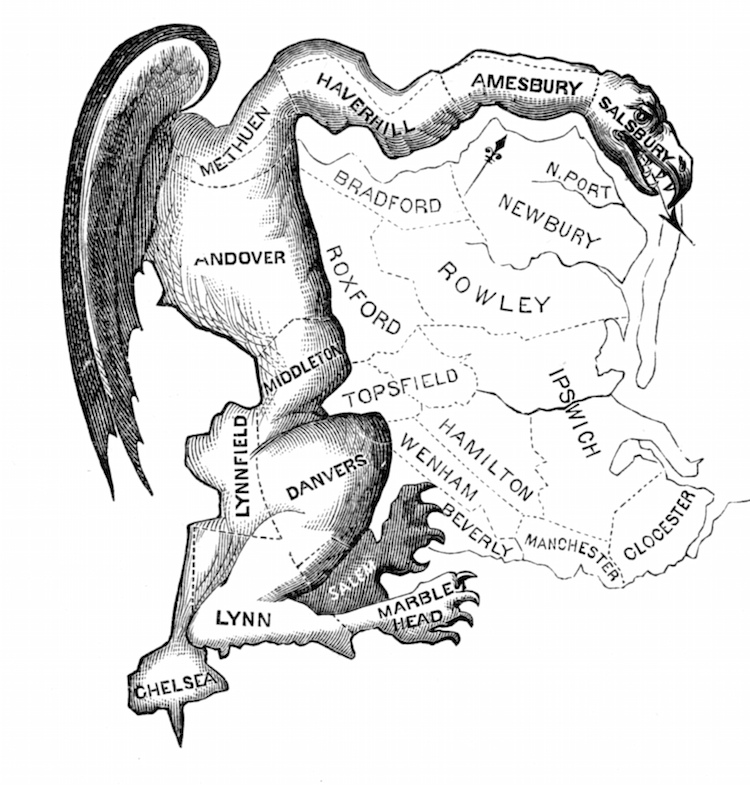
\includegraphics[width=.5\columnwidth]{gerrymander}%
\label{fig:gerrymander}%
%\end{figure}
%\end{wrapfigure}
\end{tabular}


Consider the simple state\footnote{Diagrams adapted from Stephen Nass, ``How to Steal an Election''}: 
\newcommand{\district}{
	%locations of participants
	\begin{scope}[shift = {(-.1, -.1)}]
			\draw[very thick] (0,0) -- (10,0) -- (10,5) -- (0,5) -- cycle;
	\end{scope}
	 \foreach \y in {0,1}
	 \foreach \x in {0,1,2,3,4,5,6,7,8,9}
    \draw[teal, opacity = .2, fill = teal] (\x,\y) rectangle (\x+.8,\y+.8);
	 \foreach \y in {2,3,4}
	 \foreach \x in {0,1,2,3,4,5,6,7,8,9}
    \draw[orange, fill=orange] (\x,\y) rectangle (\x+.8,\y+.8);
}

%\begin{wrapfigure}{l}{.5\columnwidth}
\begin{center}
	\begin{tikzpicture}[scale=.5]
	\district
\end{tikzpicture}
\end{center}
%\end{wrapfigure}

There are 50 people in this state who belong to two different political parties.  The census says that they should have 5 seats, so we need to divide up these people into 5 groups.  
\begin{enumerate}
	 \begin{tabular}{m{.45\textwidth}m{.45\textwidth}}
	 \item Consider the following districting of this state. Who would win with a majority of votes in each district?  Who has an advantage in the legislature?  Does it seem fair? Are the people in each district connected to each other?  Are the districts generally compact? &\newcommand{\districta}{\begin{scope}[shift = {(-.1,-.1)}]
		\draw[very thick] (0,0 ) -- (10, 0 );
		\draw[very thick] (0,1 ) -- (10, 1 );
		\draw[very thick] (0,2 ) -- (10, 2 );
		\draw[very thick] (0,3 ) -- (10, 3 );
		\draw[very thick] (0,4 ) -- (10, 4 );
		\end{scope}}
	
	\begin{tikzpicture}[scale=.5]
		\district 
		\begin{scope}[shift = {(-.1,-.1)}]
			\draw[very thick] (0,0 ) -- (10, 0 );
		\draw[very thick] (0,1 ) -- (10, 1 );
		\draw[very thick] (0,2 ) -- (10, 2 );
		\draw[very thick] (0,3 ) -- (10, 3 );
		\draw[very thick] (0,4 ) -- (10, 4 );
		\end{scope}
			\end{tikzpicture} 
	 
	\end{tabular}
	
	
	\vfill
	\clearpage
	 \begin{tabular}{m{.45\textwidth}m{.45\textwidth}}
	 \item Consider the following districting of this state. Who would win with a majority of votes in each district?  Who has an advantage in the legislature?  Does it seem fair? Are the people in each district connected to each other?  Are the districts generally compact? &
	\newcommand{\districtb}{	
	\begin{scope}[shift={(-.1,-.1)}]
					\foreach \x in {0,2,4,6,8}
	\draw[very thick] (\x,0) -- (\x, 5);

	\end{scope}
	}\begin{tikzpicture}[scale=.5]
	\district
	\districtb
	\end{tikzpicture}
	\end{tabular}
	 
	\vfill
 \begin{tabular}{m{.5\textwidth}m{.5\textwidth}}
	 \item Consider the following districting of this state. Who would win with a majority of votes in each district?  Who has an advantage in the legislature?  Does it seem fair? Are the people in each district connected to each other?  Are the districts generally compact? &
		\newcommand{\districtc}{
		\begin{scope}[shift = {(-.1, -.1)}]
				\draw[very thick] (0,0) -- (0,1) -- (1,1) -- (1,4) -- (3,4) -- (3,1) -- (4,1) -- (4,0);
				\draw[very thick] (3,4) -- (4,4) -- (4,2) -- (5, 2) -- (5,5);
				\draw[very thick] (5, 2) -- (6,2) -- (6,4) -- (9,4) -- (9, 1) -- (10, 1);
				\draw[very thick] (7,4) -- (7,1) -- (6,1) -- (6,0);
		\end{scope}
}

\begin{tikzpicture}[scale=.5]
\district
	\districtc	
	\end{tikzpicture} \end{tabular}
	 
	\vfill

	

The last diagram is an example of the `packing' and `cracking' that are illustrative of modern gerrymandering.
\begin{description}
	\item[packing] Putting a very large number of voters who all vote the same way in a single district.  In this case, the election is won by these voters, but by a very large margin.\index{gerrymander!packing}
	\item[cracking] Putting a slight majority of voters for one party in a single district.  In this case, the election is won by these voters by a slim margin.  There are a lot of minority voters in the district, but not enough to ever win an election.\index{gerrymander!cracking}
\end{description}
\clearpage

\item The state below has approximately 40\% orange (\tikz{\draw[fill=orange,orange]  circle(1ex);}) people and 60\% teal (\tikz{\draw[fill=teal,teal, opacity = .2]  circle(1ex);}) people (each color was selected randomly).  Divide the state into 10 districts in such a way so that in an election 40\% of the seats will be won by the orange people and 60\% by the teal people.

\newcommand{\firstexample}{	\begin{scope}[shift = {(-.9, -.9)}]
\draw[teal, fill = teal, opacity = 0.4] (1, 1) rectangle (1.8, 1.8);	\draw[orange, fill = orange] (1, 2) rectangle (1.8, 2.8);	\draw[orange, fill = orange] (1, 3) rectangle (1.8, 3.8);	\draw[orange, fill = orange] (1, 4) rectangle (1.8, 4.8);	\draw[teal, fill = teal, opacity = 0.4] (1, 5) rectangle (1.8, 5.8);	\draw[orange, fill = orange] (1, 6) rectangle (1.8, 6.8);	\draw[orange, fill = orange] (1, 7) rectangle (1.8, 7.8);	\draw[teal, fill = teal, opacity = 0.4] (1, 8) rectangle (1.8, 8.8);	\draw[orange, fill = orange] (1, 9) rectangle (1.8, 9.8);	\draw[orange, fill = orange] (1, 10) rectangle (1.8, 10.8);
\draw[teal, fill = teal, opacity = 0.4] (2, 1) rectangle (2.8, 1.8);	\draw[teal, fill = teal, opacity = 0.4] (2, 2) rectangle (2.8, 2.8);	\draw[teal, fill = teal, opacity = 0.4] (2, 3) rectangle (2.8, 3.8);	\draw[teal, fill = teal, opacity = 0.4] (2, 4) rectangle (2.8, 4.8);	\draw[teal, fill = teal, opacity = 0.4] (2, 5) rectangle (2.8, 5.8);	\draw[orange, fill = orange] (2, 6) rectangle (2.8, 6.8);	\draw[teal, fill = teal, opacity = 0.4] (2, 7) rectangle (2.8, 7.8);	\draw[orange, fill = orange] (2, 8) rectangle (2.8, 8.8);	\draw[teal, fill = teal, opacity = 0.4] (2, 9) rectangle (2.8, 9.8);	\draw[teal, fill = teal, opacity = 0.4] (2, 10) rectangle (2.8, 10.8);
\draw[teal, fill = teal, opacity = 0.4] (3, 1) rectangle (3.8, 1.8);	\draw[teal, fill = teal, opacity = 0.4] (3, 2) rectangle (3.8, 2.8);	\draw[teal, fill = teal, opacity = 0.4] (3, 3) rectangle (3.8, 3.8);	\draw[teal, fill = teal, opacity = 0.4] (3, 4) rectangle (3.8, 4.8);	\draw[teal, fill = teal, opacity = 0.4] (3, 5) rectangle (3.8, 5.8);	\draw[orange, fill = orange] (3, 6) rectangle (3.8, 6.8);	\draw[orange, fill = orange] (3, 7) rectangle (3.8, 7.8);	\draw[teal, fill = teal, opacity = 0.4] (3, 8) rectangle (3.8, 8.8);	\draw[teal, fill = teal, opacity = 0.4] (3, 9) rectangle (3.8, 9.8);	\draw[teal, fill = teal, opacity = 0.4] (3, 10) rectangle (3.8, 10.8);
\draw[orange, fill = orange] (4, 1) rectangle (4.8, 1.8);	\draw[teal, fill = teal, opacity = 0.4] (4, 2) rectangle (4.8, 2.8);	\draw[teal, fill = teal, opacity = 0.4] (4, 3) rectangle (4.8, 3.8);	\draw[teal, fill = teal, opacity = 0.4] (4, 4) rectangle (4.8, 4.8);	\draw[orange, fill = orange] (4, 5) rectangle (4.8, 5.8);	\draw[orange, fill = orange] (4, 6) rectangle (4.8, 6.8);	\draw[orange, fill = orange] (4, 7) rectangle (4.8, 7.8);	\draw[teal, fill = teal, opacity = 0.4] (4, 8) rectangle (4.8, 8.8);	\draw[teal, fill = teal, opacity = 0.4] (4, 9) rectangle (4.8, 9.8);	\draw[teal, fill = teal, opacity = 0.4] (4, 10) rectangle (4.8, 10.8);
\draw[teal, fill = teal, opacity = 0.4] (5, 1) rectangle (5.8, 1.8);	\draw[orange, fill = orange] (5, 2) rectangle (5.8, 2.8);	\draw[teal, fill = teal, opacity = 0.4] (5, 3) rectangle (5.8, 3.8);	\draw[teal, fill = teal, opacity = 0.4] (5, 4) rectangle (5.8, 4.8);	\draw[orange, fill = orange] (5, 5) rectangle (5.8, 5.8);	\draw[teal, fill = teal, opacity = 0.4] (5, 6) rectangle (5.8, 6.8);	\draw[teal, fill = teal, opacity = 0.4] (5, 7) rectangle (5.8, 7.8);	\draw[teal, fill = teal, opacity = 0.4] (5, 8) rectangle (5.8, 8.8);	\draw[teal, fill = teal, opacity = 0.4] (5, 9) rectangle (5.8, 9.8);	\draw[teal, fill = teal, opacity = 0.4] (5, 10) rectangle (5.8, 10.8);
\draw[orange, fill = orange] (6, 1) rectangle (6.8, 1.8);	\draw[teal, fill = teal, opacity = 0.4] (6, 2) rectangle (6.8, 2.8);	\draw[orange, fill = orange] (6, 3) rectangle (6.8, 3.8);	\draw[teal, fill = teal, opacity = 0.4] (6, 4) rectangle (6.8, 4.8);	\draw[orange, fill = orange] (6, 5) rectangle (6.8, 5.8);	\draw[teal, fill = teal, opacity = 0.4] (6, 6) rectangle (6.8, 6.8);	\draw[orange, fill = orange] (6, 7) rectangle (6.8, 7.8);	\draw[orange, fill = orange] (6, 8) rectangle (6.8, 8.8);	\draw[orange, fill = orange] (6, 9) rectangle (6.8, 9.8);	\draw[orange, fill = orange] (6, 10) rectangle (6.8, 10.8);
\draw[teal, fill = teal, opacity = 0.4] (7, 1) rectangle (7.8, 1.8);	\draw[teal, fill = teal, opacity = 0.4] (7, 2) rectangle (7.8, 2.8);	\draw[teal, fill = teal, opacity = 0.4] (7, 3) rectangle (7.8, 3.8);	\draw[teal, fill = teal, opacity = 0.4] (7, 4) rectangle (7.8, 4.8);	\draw[teal, fill = teal, opacity = 0.4] (7, 5) rectangle (7.8, 5.8);	\draw[teal, fill = teal, opacity = 0.4] (7, 6) rectangle (7.8, 6.8);	\draw[teal, fill = teal, opacity = 0.4] (7, 7) rectangle (7.8, 7.8);	\draw[orange, fill = orange] (7, 8) rectangle (7.8, 8.8);	\draw[orange, fill = orange] (7, 9) rectangle (7.8, 9.8);	\draw[teal, fill = teal, opacity = 0.4] (7, 10) rectangle (7.8, 10.8);
\draw[teal, fill = teal, opacity = 0.4] (8, 1) rectangle (8.8, 1.8);	\draw[orange, fill = orange] (8, 2) rectangle (8.8, 2.8);	\draw[teal, fill = teal, opacity = 0.4] (8, 3) rectangle (8.8, 3.8);	\draw[teal, fill = teal, opacity = 0.4] (8, 4) rectangle (8.8, 4.8);	\draw[teal, fill = teal, opacity = 0.4] (8, 5) rectangle (8.8, 5.8);	\draw[orange, fill = orange] (8, 6) rectangle (8.8, 6.8);	\draw[orange, fill = orange] (8, 7) rectangle (8.8, 7.8);	\draw[orange, fill = orange] (8, 8) rectangle (8.8, 8.8);	\draw[teal, fill = teal, opacity = 0.4] (8, 9) rectangle (8.8, 9.8);	\draw[orange, fill = orange] (8, 10) rectangle (8.8, 10.8);
\draw[teal, fill = teal, opacity = 0.4] (9, 1) rectangle (9.8, 1.8);	\draw[orange, fill = orange] (9, 2) rectangle (9.8, 2.8);	\draw[orange, fill = orange] (9, 3) rectangle (9.8, 3.8);	\draw[teal, fill = teal, opacity = 0.4] (9, 4) rectangle (9.8, 4.8);	\draw[orange, fill = orange] (9, 5) rectangle (9.8, 5.8);	\draw[orange, fill = orange] (9, 6) rectangle (9.8, 6.8);	\draw[teal, fill = teal, opacity = 0.4] (9, 7) rectangle (9.8, 7.8);	\draw[orange, fill = orange] (9, 8) rectangle (9.8, 8.8);	\draw[teal, fill = teal, opacity = 0.4] (9, 9) rectangle (9.8, 9.8);	\draw[teal, fill = teal, opacity = 0.4] (9, 10) rectangle (9.8, 10.8);
\draw[orange, fill = orange] (10, 1) rectangle (10.8, 1.8);	\draw[teal, fill = teal, opacity = 0.4] (10, 2) rectangle (10.8, 2.8);	\draw[teal, fill = teal, opacity = 0.4] (10, 3) rectangle (10.8, 3.8);	\draw[orange, fill = orange] (10, 4) rectangle (10.8, 4.8);	\draw[teal, fill = teal, opacity = 0.4] (10, 5) rectangle (10.8, 5.8);	\draw[teal, fill = teal, opacity = 0.4] (10, 6) rectangle (10.8, 6.8);	\draw[orange, fill = orange] (10, 7) rectangle (10.8, 7.8);	\draw[teal, fill = teal, opacity = 0.4] (10, 8) rectangle (10.8, 8.8);	\draw[teal, fill = teal, opacity = 0.4] (10, 9) rectangle (10.8, 9.8);	\draw[orange, fill = orange] (10, 10) rectangle (10.8, 10.8);

	\end{scope}
}
\begin{tikzpicture}[scale=.75]
	\firstexample
	\begin{scope}[]
		\draw[very thick] (0,0) -- (0,10) -- (10,10) -- (10,0) -- cycle;
	\end{scope}
\end{tikzpicture}
\vfill

\item Now, divide the same state in such a way so that 60\% of the seats will be won by the orange people.\\
\begin{tikzpicture}[scale = .75]
	\firstexample
	\begin{scope}[]
		\draw[very thick] (0,0) -- (0,10) -- (10,10) -- (10,0) -- cycle;
	\end{scope}
\end{tikzpicture}
\vfill

\end{enumerate}
%<*HWHEADER>
\clearpage
%%%%%%%%%%%%%%%%%%%%%%%%%%%%%%%%%%%%%%%%%%%%%%%%%%%%%%%%%%%%%%%%%%%%%%%%%%%%%%%%%%%%%%%%%%%%%%%%%%%%%%%%
\HOMEWORK
%</HWHEADER>

%<*HOMEWORK>


\begin{Renumerate}

  \item Consider the following map.  Put 5 districts on the map so that orange receives the most seats.
	\newcommand{\homeworkone}{
		\begin{scope}[shift = {(-.9,-.9)}]
			\draw[orange, fill = orange] (1, 1) rectangle (1.8, 1.8);	
			\draw[teal, fill = teal, opacity = 0.4] (1, 2) rectangle (1.8, 2.8);	
			\draw[teal, fill = teal, opacity = 0.4] (1, 3) rectangle (1.8, 3.8);	
			\draw[teal, fill = teal, opacity = 0.4] (1, 4) rectangle (1.8, 4.8);	
			\draw[orange, fill = orange] (1, 5) rectangle (1.8, 5.8);
			\draw[orange, fill = orange] (2, 1) rectangle (2.8, 1.8);	
			\draw[teal, fill = teal, opacity = 0.4] (2, 2) rectangle (2.8, 2.8);	
			\draw[teal, fill = teal, opacity = 0.4] (2, 3) rectangle (2.8, 3.8);	
			\draw[teal, fill = teal, opacity = 0.4] (2, 4) rectangle (2.8, 4.8);	
			\draw[teal, fill = teal, opacity = 0.4] (2, 5) rectangle (2.8, 5.8);
			\draw[teal, fill = teal, opacity = 0.4] (3, 1) rectangle (3.8, 1.8);	
			\draw[orange, fill = orange] (3, 2) rectangle (3.8, 2.8);	
			\draw[teal, fill = teal, opacity = 0.4] (3, 3) rectangle (3.8, 3.8);	
			\draw[teal, fill = teal, opacity = 0.4] (3, 4) rectangle (3.8, 4.8);	
			\draw[teal, fill = teal, opacity = 0.4] (3, 5) rectangle (3.8, 5.8);
			\draw[orange, fill = orange] (4, 1) rectangle (4.8, 1.8);	
			\draw[orange, fill = orange] (4, 2) rectangle (4.8, 2.8);	
			\draw[orange, fill = orange] (4, 3) rectangle (4.8, 3.8);	
			\draw[orange, fill = orange] (4, 4) rectangle (4.8, 4.8);	
			\draw[teal, fill = teal, opacity = 0.4] (4, 5) rectangle (4.8, 5.8);
			\draw[teal, fill = teal, opacity = 0.4] (5, 1) rectangle (5.8, 1.8);	
			\draw[teal, fill = teal, opacity = 0.4] (5, 2) rectangle (5.8, 2.8);	
			\draw[orange, fill = orange] (5, 3) rectangle (5.8, 3.8);	
			\draw[teal, fill = teal, opacity = 0.4] (5, 4) rectangle (5.8, 4.8);	
			\draw[orange, fill = orange] (5, 5) rectangle (5.8, 5.8);
	\end{scope}
}
	
\begin{center}
		\begin{tikzpicture}
		\homeworkone
		\begin{scope}
			\draw[very thick] (0,0) -- (0,5) -- (5,5) -- (5,0)  --cycle;
		\end{scope}
	\end{tikzpicture}

\end{center}	
	\item Put 5 districts on the map so that teal receives the most districts.
	
\begin{center}
			\begin{tikzpicture}
		\homeworkone
		
		\begin{scope}
			\draw[very thick] (0,0) -- (0,5) -- (5,5) -- (5,0)  --cycle;
		\end{scope}
	\end{tikzpicture}

\end{center}
\end{Renumerate} 

\ENDHOMEWORK

%%%%%%%%%%%%%%%%%%%%%%%%%%%%%%%%%%%%%%%%%%%%%%%%%%%%%%%%%%%%%%%%%%%%%%%%%%%%%%%%%%%%%%%%%%%%%

\clearpage

\section{Fairness}
The big question of the day is 
\begin{quote}
Justice Kennedy suggested, as he did in another redistricting case 13 years ago, that courts perhaps could be involved in placing limits on extremely partisan electoral maps.  13 years ago he wrote "If courts refuse to entertain any claims of partisan gerrymandering, the temptation to use partisan favoritism in districting in an unconstitutional manner will grow," 
\end{quote}

\subsection{Geometric Measures} \index{redistricting:geometric measures of fairness}
Although most states have a requirement that their districts be compact, there is no good definition for how compact a set of districts would be.  We will look at two different ways of measuring compactness.  To make measurement easier, we will be using our example districts from before.

\subsubsection{Area vs. Perimeter}
One way of measuring how compact a district is comes from dividing the area of the district by its perimeter squared and then multiplying by 16\footnote{You multiply by 16 because the Isoperimetric measure for a square is $\frac{1}{16}$ and we would like our ratio to be about 1.}.  In general, this type of calculation is known as an Isoperimetric measure. \index{redistricting!isoperimetric measure}
\begin{enumerate}
	\item Example:
\begin{center}
		\begin{tikzpicture}[scale=.5]
		begin{scope}
		 \draw[orange, fill=orange] (0,0) rectangle (.8,.8);
		\draw[orange, fill=orange] (0,1) rectangle (.8,1+.8);
		\draw[orange, fill=orange] (0,2) rectangle (.8,2+.8);
		\draw[teal, opacity = .2, fill=teal] (1,0) rectangle (1+.8, .8);
		\draw[teal, opacity = .2, fill=teal] (1,1) rectangle (1+.8, 1+.8);
			\begin{scope}[shift = {(-.1, -.1)}]
			\draw[very thick] (0,0) -- (2,0) -- (2,2) -- (1,2) -- (1, 3) -- (0,3) -- cycle;
			
			\node at (6,2) {Area = 5};
			\node at (6,1) {Perimeter = 10 };
			\node at (14,2) {Ratio $= \frac{16\cdot5}{10^2} = 0.8$};
			\end{scope}
	\end{tikzpicture}
\end{center}
 \textbf{Notes.}         \fillwithlines{\stretch{1}}

\clearpage
\begin{tikzpicture}[scale=.5]
	\begin{scope}
			\district 
			\begin{scope}[shift = {(-.1,-.1)}]
		\draw[very thick] (0,0 ) -- (10, 0 );
		\draw[very thick] (0,1 ) -- (10, 1 );
		\draw[very thick] (0,2 ) -- (10, 2 );
		\draw[very thick] (0,3 ) -- (10, 3 );
		\draw[very thick] (0,4 ) -- (10, 4 );
		\end{scope}
		\begin{scope}[shift = {(.4,.4)}]
			\node at (0,0) {\textbf{E}};
			\node at (0,1) {\textbf{D}};
			\node at (0,2) {\textbf{C}};
			\node at (0,3) {\textbf{B}};
			\node at (0,4) {\textbf{A}};
		\end{scope}
			
			\node at (5,-2) {\textbf{Redistricting Plan 1}};
	\end{scope}
	
	\begin{scope}[shift = {(4.5in,0)}]
		\district 
		\begin{scope}[shift={(-.1,-.1)}]
					\foreach \x in {0,2,4,6,8}
	\draw[very thick] (\x,0) -- (\x, 5);

	\end{scope}
	
		\begin{scope}[shift={(.4,.4)}]
			\node at (0,0) {\textbf{A}};
			\node at (2,0) {\textbf{B}};
			\node at (4,0) {\textbf{C}};
			\node at (6,0) {\textbf{D}};
			\node at (8,0) {\textbf{E}};
		\end{scope}
			
			\node at (5,-2) {\textbf{Redistricting Plan 2}};
	\end{scope}
	
	\begin{scope}[shift = {(9in,0)}]
	\district 
		\begin{scope}[shift = {(-.1, -.1)}]
				\draw[very thick] (0,0) -- (0,1) -- (1,1) -- (1,4) -- (3,4) -- (3,1) -- (4,1) -- (4,0);
				\draw[very thick] (3,4) -- (4,4) -- (4,2) -- (5, 2) -- (5,5);
				\draw[very thick] (5, 2) -- (6,2) -- (6,4) -- (9,4) -- (9, 1) -- (10, 1);
				\draw[very thick] (7,4) -- (7,1) -- (6,1) -- (6,0);
		\end{scope}
			\begin{scope}[shift = {(.4,.4)}]
				\node at (0,1) {\textbf{A}};
			\node at (0,0) {\textbf{B}};
			\node at (4,0) {\textbf{C}};
			\node at (5,2) {\textbf{D}};
			\node at (6,0) {\textbf{E}};
			\end{scope}
			
			\node at (5,-2) {\textbf{Redistricting Plan 3}};
	\end{scope}
\end{tikzpicture}

\item Calculate the area and perimeter of each district for each plan.  Fill in the table below.
\begin{center} \renewcommand{\arraystretch}{1.5}
	\begin{tabular}{|cc||cc||cc|} \hline
	Plan 1 & $16\frac{\text{Area}}{\text{Perimeter}^2}$ & Plan 2 & $16\frac{\text{Area}}{\text{Perimeter}^2}$ & Plan 3 & $16\frac{\text{Area}}{\text{Perimeter}^2}$\\\hline
	District A & & District A & &District A & \\\hline
	District B & & District B & &District B & \\\hline
	District C & & District C & &District C & \\\hline
	District D & & District D & &District D & \\\hline
	District E & & District E & &District E & \\\hline
	Average && Average && Average &\\\hline
	\end{tabular}
\end{center}

\item Does the calculation differentiate between the plans?  Does it show one plan as being ``better'' than the others?   
 \fillwithlines{\stretch{1}}

\subsubsection{Enclosing Square}
Another way of measuring how compact a district is comes from thinking of placing the district into the smallest square that contains the district.  Then you calculate the area of the district and its' enclosing square and divide the first by the second.  Generally, this type of calculation is known as a Reock measure. \index{redistricting!Reock measure}  For example:
\begin{center}
	\begin{tikzpicture}[scale=.5]
		\begin{scope}
		\draw[orange, fill=orange] (0,0) rectangle (.8,.8);
		\draw[orange, fill=orange] (0,1) rectangle (.8,1.8);
		\draw[orange, fill=orange] (0,2) rectangle (.8,2.8);
		\draw[teal, opacity = .2, fill=teal] (1,0) rectangle (1.8,.8);
		\draw[teal, opacity = .2, fill=teal] (1,1) rectangle (1.8,1.8);
			\begin{scope}[shift = {(-.1, -.1)}]
			\draw[very thick] (0,0) -- (2,0) -- (2,2) -- (1,2) -- (1, 3) -- (0,3) -- cycle;
			
			\node at (6,2) {Area = 5};
			\end{scope}
		\end{scope}
		%\node at (4in,3) {vs.};
		\node at (4in,0) {Ratio = $\frac{5}{9}=0.56$};
		\begin{scope}[shift = {(6in,0)}]
		\draw[orange, fill=orange] (0,0) rectangle (.8,.8);
		\draw[orange, fill=orange] (0,1) rectangle (.8,1.8);
		\draw[orange, fill=orange] (0,2) rectangle (.8,2.8);
		\draw[teal, opacity = .2, fill=teal] (1,0) rectangle (1.8,.8);
		\draw[teal, opacity = .2, fill=teal] (1,1) rectangle (1.8,1.8);
			\begin{scope}[shift = {(-.1, -.1)}]
			\draw[very thick] (0,0) -- (3,0) -- (3,3) -- (0,3) -- cycle;
			\node at (6,2) {Area = 9};
			
			\end{scope}
		\end{scope}
	\end{tikzpicture}
\end{center}

\item 
 \textbf{Notes.}         \fillwithlines{\stretch{1}}

\clearpage
\begin{tikzpicture}[scale=.5]
	\begin{scope}
			\district 
			\begin{scope}[shift = {(-.1,-.1)}]
		\draw[very thick] (0,0 ) -- (10, 0 );
		\draw[very thick] (0,1 ) -- (10, 1 );
		\draw[very thick] (0,2 ) -- (10, 2 );
		\draw[very thick] (0,3 ) -- (10, 3 );
		\draw[very thick] (0,4 ) -- (10, 4 );
		\end{scope}
		\begin{scope}[shift = {(.4,.4)}]
			\node at (0,0) {\textbf{E}};
			\node at (0,1) {\textbf{D}};
			\node at (0,2) {\textbf{C}};
			\node at (0,3) {\textbf{B}};
			\node at (0,4) {\textbf{A}};
		\end{scope}
			
			\node at (5,-2) {\textbf{Redistricting Plan 1}};
	\end{scope}
	
	\begin{scope}[shift = {(4.5in,0)}]
		\district 
		\begin{scope}[shift={(-.1,-.1)}]
					\foreach \x in {0,2,4,6,8}
	\draw[very thick] (\x,0) -- (\x, 5);

	\end{scope}
	
		\begin{scope}[shift={(.4,.4)}]
			\node at (0,0) {\textbf{A}};
			\node at (2,0) {\textbf{B}};
			\node at (4,0) {\textbf{C}};
			\node at (6,0) {\textbf{D}};
			\node at (8,0) {\textbf{E}};
		\end{scope}
			
			\node at (5,-2) {\textbf{Redistricting Plan 2}};
	\end{scope}
	
	\begin{scope}[shift = {(9in,0)}]
	\district 
		\begin{scope}[shift = {(-.1, -.1)}]
				\draw[very thick] (0,0) -- (0,1) -- (1,1) -- (1,4) -- (3,4) -- (3,1) -- (4,1) -- (4,0);
				\draw[very thick] (3,4) -- (4,4) -- (4,2) -- (5, 2) -- (5,5);
				\draw[very thick] (5, 2) -- (6,2) -- (6,4) -- (9,4) -- (9, 1) -- (10, 1);
				\draw[very thick] (7,4) -- (7,1) -- (6,1) -- (6,0);
		\end{scope}
			\begin{scope}[shift = {(.4,.4)}]
				\node at (0,1) {\textbf{A}};
			\node at (0,0) {\textbf{B}};
			\node at (4,0) {\textbf{C}};
			\node at (5,2) {\textbf{D}};
			\node at (6,0) {\textbf{E}};
			\end{scope}
			
			\node at (5,-2) {\textbf{Redistricting Plan 3}};
	\end{scope}
\end{tikzpicture}

\item Calculate the area and perimeter of each district for each plan.  Fill in the table below.
\begin{center} \renewcommand{\arraystretch}{1.5}
	\begin{tabular}{|cc||cc||cc|} \hline
	Plan 1 & $\frac{\text{Area District}}{\text{Area square}}$ & Plan 2 & $\frac{\text{Area District}}{\text{Area square}}$ & Plan 3 & $\frac{\text{Area District}}{\text{Area square}}$\\\hline
	District A & & District A & &District A & \\\hline
	District B & & District B & &District B & \\\hline
	District C & & District C & &District C & \\\hline
	District D & & District D & &District D & \\\hline
	District E & & District E & &District E & \\\hline
	Average && Average && Average &\\\hline
	\end{tabular}
\end{center}

\item Does the calculation differentiate between the plans?  Does it show one plan as being ``better'' than the others?   
 \fillwithlines{\stretch{1}}
\item If you were asked to chose which method better differentiates your notion of compact, which would you use and why?
\fillwithlines{\stretch{1}}

%<*HWHEADER>
\clearpage
%%%%%%%%%%%%%%%%%%%%%%%%%%%%%%%%%%%%%%%%%%%%%%%%%%%%%%%%%%%%%%%%%%%%%%%%%%%%%%%%%%%%%%%%%%%%%%%%%%%%%%%%
\HOMEWORK
%</HWHEADER>

%<*HOMEWORK>


\begin{Renumerate}

  \item Go back to the 5 districts you drew on the map (or draw new ones) so that orange receives the most seats. What is your average calculation for $\frac{16\text{area}}{\text{perimeter}^2}$?  What is your average calculation for $\frac{\text{area of district}}{\text{area of enclosing square}}$?
	\newcommand{\homeworkone}{\begin{scope}[shift = {(-.9,-.9)}]
\draw[orange, fill = orange] (1, 1) rectangle (1.8, 1.8);	\draw[teal, fill = teal, opacity = 0.4] (1, 2) rectangle (1.8, 2.8);	\draw[teal, fill = teal, opacity = 0.4] (1, 3) rectangle (1.8, 3.8);	\draw[teal, fill = teal, opacity = 0.4] (1, 4) rectangle (1.8, 4.8);	\draw[orange, fill = orange] (1, 5) rectangle (1.8, 5.8);
\draw[orange, fill = orange] (2, 1) rectangle (2.8, 1.8);	\draw[teal, fill = teal, opacity = 0.4] (2, 2) rectangle (2.8, 2.8);	\draw[teal, fill = teal, opacity = 0.4] (2, 3) rectangle (2.8, 3.8);	\draw[teal, fill = teal, opacity = 0.4] (2, 4) rectangle (2.8, 4.8);	\draw[teal, fill = teal, opacity = 0.4] (2, 5) rectangle (2.8, 5.8);
\draw[teal, fill = teal, opacity = 0.4] (3, 1) rectangle (3.8, 1.8);	\draw[orange, fill = orange] (3, 2) rectangle (3.8, 2.8);	\draw[teal, fill = teal, opacity = 0.4] (3, 3) rectangle (3.8, 3.8);	\draw[teal, fill = teal, opacity = 0.4] (3, 4) rectangle (3.8, 4.8);	\draw[teal, fill = teal, opacity = 0.4] (3, 5) rectangle (3.8, 5.8);
\draw[orange, fill = orange] (4, 1) rectangle (4.8, 1.8);	\draw[orange, fill = orange] (4, 2) rectangle (4.8, 2.8);	\draw[orange, fill = orange] (4, 3) rectangle (4.8, 3.8);	\draw[orange, fill = orange] (4, 4) rectangle (4.8, 4.8);	\draw[teal, fill = teal, opacity = 0.4] (4, 5) rectangle (4.8, 5.8);
\draw[teal, fill = teal, opacity = 0.4] (5, 1) rectangle (5.8, 1.8);	\draw[teal, fill = teal, opacity = 0.4] (5, 2) rectangle (5.8, 2.8);	\draw[orange, fill = orange] (5, 3) rectangle (5.8, 3.8);	\draw[teal, fill = teal, opacity = 0.4] (5, 4) rectangle (5.8, 4.8);	\draw[orange, fill = orange] (5, 5) rectangle (5.8, 5.8);
	\end{scope}}
	
\begin{center}
		\begin{tikzpicture}
		\homeworkone
		
		\begin{scope}
			\draw[very thick] (0,0) -- (0,5) -- (5,5) -- (5,0)  --cycle;
		\end{scope}
	\end{tikzpicture}

\end{center}	
	\item Go back to the 5 districts you drew on the map (or draw new ones) so that teal receives the most seats. What is your average calculation for $\frac{16\text{area}}{\text{perimeter}^2}$?  What is your average calculation for $\frac{\text{area of district}}{\text{area of enclosing square}}$?
	
\begin{center}
			\begin{tikzpicture}
		\homeworkone
		
		\begin{scope}
			\draw[very thick] (0,0) -- (0,5) -- (5,5) -- (5,0)  --cycle;
		\end{scope}
	\end{tikzpicture}

\end{center}

\item Does the average of $\frac{16\text{area}}{\text{perimeter}^2}$ demonstrate unfairness in either of your plans? \vfill

\item Does the average of $\frac{\text{area of enclosing square}}{\text{area of district}}$ demonstrate unfairness in either of your plans? \vfill

\end{Renumerate} 

\ENDHOMEWORK

%%%%%%%%%%%%%%%%%%%%%%%%%%%%%%%%%%%%%%%%%%%%%%%%%%%%%%%%%%%%%%%%%%%%%%%%%%%%%%%%%%%%%%%%%%%%%

\clearpage
\subsection{Arithmetic Measures}\index{redistricting!arithmetic measures of fairness}
Okay, so maybe just looking geometrically at how the districts are drawn is not a good way of testing how fair a redistricting is.  Maybe there is something about the election and where the people who live in the district are placed that would help us measure the fairness of the redistricting plan.
\subsubsection{Efficiency Gap} \index{redistricting!efficiency gap} \index{gerrymander!efficiency gap}
A state has been divided into 5 districts of 100 voters each.  Each district votes to elect a representative from one of two parties, $A$ or $B$.  In any election, many voters will end up feeling that voting was a waste of their time.  A voter could feel this way for two reasons:
\begin{itemize}
	\item Her party lost, so what was the point of showing up to vote?
	\item Her party won by a landslide, so what was the point of showing up to vote?
\end{itemize}
Corresponding to this, we will count:
\begin{itemize}
	\item All of the votes for party $A$ as wasted if party $A$ looses.
	\item All of the votes above 50\% for party $A$ as wasted if party $A$ wins.
\end{itemize}
\item Complete the following table (we will use $W_A$ as a short cut for the votes wasted by party $A$.):
\begin{center}
	\begin{tabular}{|c||c|c|p{2cm}||p{1.5cm}|p{1.5cm}||p{2cm}|p{2cm}|}\hline
	District & A votes & B votes & Winner & $W_A$ & $W_B$ & $W_A+W_B$ & $W_A-W_B$\\\hline\hline\ifsolns
	1 & 95 & 5 & A & 45 & 5 & 50 & 40\\ \hline 
2 & 40 & 60 & B & 40 & 10 & 50 & 30\\ \hline 
3 & 75 & 25 & A & 25 & 25 & 50 & 0\\ \hline 
4 & 45 & 55 & B & 45 & 5 & 50 & 40\\ \hline 
5 & 45 & 55 & B & 45 & 5 & 50 & 40\\ \hline \hline 
	TOTAL & 300 & 200 & $A$: 2 $B$:3   & 200 & 50 & 250 & 150\\\hline
		\else
	1 & 95 & 5 & $A$ & 45 & 5 & 50 & 40\\\hline
	2 & 40 & 60 &  &  &  &  & \\\hline
	3 & 75 & 25 &  &  &  &  & \\\hline
	4 & 45 & 55 &  &  &  &  & \\\hline
	5 & 45 & 55 &  &  &  &  & \\\hline \hline
	TOTAL & 300 & 200 & $A$: \hspace{.75cm} $B$:\hspace{.75cm}   &  &  &  & \\\hline\fi
	\end{tabular}
\end{center}
The \textbf{Efficiency Gap} is defined to be the fraction of the difference of wasted votes divided by the total number of votes: \index{Efficiency Gap}
\[ \text{EG} = \frac{W_A-W_B}{\text{Votes}} =\]
The $V$ in the denominator normalized EG, so that its magnitude does not depend on the population of the state.  The idea is that when EG is much larger than 0, the districting plan may be unfair to party $A$, because $A$ is wasting more votes.  When EG is much smaller than 0, then $B$ is wasting more votes, so the plan may be unfair to $B$.  We do have to be careful because if a candidate is running unopposed, the efficiency gap for that election is meaningless.  We can either throw out that district in our calculations or use data from other elections to estimate what the election would look like if the seat were contested.

\item Consider the following election

\begin{center}
	\begin{tabular}{|c||c|c|p{2cm}||p{1.5cm}|p{1.5cm}||p{2cm}|p{2cm}|}\hline
	District & A votes & B votes & Winner & $W_A$ & $W_B$ & $W_A+W_B$ & $W_A-W_B$\\\hline\hline\ifsolns
		1 & 81 & 19 & A & 31 & 19 & 50 & 12\\ \hline 
		2 & 45 & 55 & B & 45 & 5 & 50 & 40\\ \hline 
		3 & 80 & 20 & A & 30 & 20 & 50 & 10\\ \hline 
		4 & 49 & 51 & B & 49 & 1 & 50 & 48\\ \hline 
		5 & 45 & 55 & B & 45 & 5 & 50 & 40\\ \hline  \hline 
	TOTAL & 300 & 200 & $A$: 2 $B$:3   & 200 & 50 & 250 & 150\\\hline
		\else
		1 & 81 & 19 &  &  &  &  & \\ \hline 
		2 & 45 & 55 &  &  &  &  & \\ \hline 
		3 & 80 & 20 &  &  &  &  & \\ \hline 
		4 & 49 & 51 &  &  &  &  & \\ \hline 
		5 & 45 & 55 &  &  &  &  &  \\ \hline \hline
	TOTAL & 300 & 200 & $A$: \hspace{.75cm} $B$:\hspace{.75cm}   &  &  &  & \\\hline\fi
	\end{tabular}
\end{center}
Fill out the table.  

\noindent Which districts show signs of \textbf{packing}, that is putting all the voters of one party together so that, although they win the district, they have a lot of wasted votes.
 \fillwithlines{\stretch{1}}
\noindent Which districts show signs of \textbf{cracking}, that is putting just enough voters of the opposing party in the district so that they are confident of winning the election and therefore the first party has a lot of wasted votes?
 \fillwithlines{\stretch{1}}

%<*HWHEADER>
\clearpage
%%%%%%%%%%%%%%%%%%%%%%%%%%%%%%%%%%%%%%%%%%%%%%%%%%%%%%%%%%%%%%%%%%%%%%%%%%%%%%%%%%%%%%%%%%%%%%%%%%%%%%%%
\HOMEWORK
%</HWHEADER>

%<*HOMEWORK>


\begin{Renumerate}

  \item Go back to the 5 districts you drew on the map (or draw new ones) so that orange receives the most seats. Assuming that each square represents 100 voters, what is the efficiency gap for your plan?
	\newcommand{\homeworkone}{\begin{scope}[shift = {(-.9,-.9)}]
\draw[orange, fill = orange] (1, 1) rectangle (1.8, 1.8);	\draw[teal, fill = teal, opacity = 0.4] (1, 2) rectangle (1.8, 2.8);	\draw[teal, fill = teal, opacity = 0.4] (1, 3) rectangle (1.8, 3.8);	\draw[teal, fill = teal, opacity = 0.4] (1, 4) rectangle (1.8, 4.8);	\draw[orange, fill = orange] (1, 5) rectangle (1.8, 5.8);
\draw[orange, fill = orange] (2, 1) rectangle (2.8, 1.8);	\draw[teal, fill = teal, opacity = 0.4] (2, 2) rectangle (2.8, 2.8);	\draw[teal, fill = teal, opacity = 0.4] (2, 3) rectangle (2.8, 3.8);	\draw[teal, fill = teal, opacity = 0.4] (2, 4) rectangle (2.8, 4.8);	\draw[teal, fill = teal, opacity = 0.4] (2, 5) rectangle (2.8, 5.8);
\draw[teal, fill = teal, opacity = 0.4] (3, 1) rectangle (3.8, 1.8);	\draw[orange, fill = orange] (3, 2) rectangle (3.8, 2.8);	\draw[teal, fill = teal, opacity = 0.4] (3, 3) rectangle (3.8, 3.8);	\draw[teal, fill = teal, opacity = 0.4] (3, 4) rectangle (3.8, 4.8);	\draw[teal, fill = teal, opacity = 0.4] (3, 5) rectangle (3.8, 5.8);
\draw[orange, fill = orange] (4, 1) rectangle (4.8, 1.8);	\draw[orange, fill = orange] (4, 2) rectangle (4.8, 2.8);	\draw[orange, fill = orange] (4, 3) rectangle (4.8, 3.8);	\draw[orange, fill = orange] (4, 4) rectangle (4.8, 4.8);	\draw[teal, fill = teal, opacity = 0.4] (4, 5) rectangle (4.8, 5.8);
\draw[teal, fill = teal, opacity = 0.4] (5, 1) rectangle (5.8, 1.8);	\draw[teal, fill = teal, opacity = 0.4] (5, 2) rectangle (5.8, 2.8);	\draw[orange, fill = orange] (5, 3) rectangle (5.8, 3.8);	\draw[teal, fill = teal, opacity = 0.4] (5, 4) rectangle (5.8, 4.8);	\draw[orange, fill = orange] (5, 5) rectangle (5.8, 5.8);
	\end{scope}}
	
\begin{center}
		\begin{tikzpicture}[scale=.5]
		\homeworkone
		
		\begin{scope}
			\draw[very thick] (0,0) -- (0,5) -- (5,5) -- (5,0)  --cycle;
		\end{scope}
	\end{tikzpicture}
	
	\begin{tabular}{|c||c|c||p{1.5cm}|p{1.5cm}||p{2cm}|}\hline
	District & O votes & T votes & $W_O$ & $W_T$ & $W_O-W_T$\\\hline\hline
	1&&&&&\\\hline
2&&&&&\\\hline
3&&&&&\\\hline
4&&&&&\\\hline
5&&&&&\\\hline
  \hline 
TOTAL &  &  &   &  & \\\hline
	\end{tabular}

\end{center}	
	\item Go back to the 5 districts you drew on the map (or draw new ones) so that teal receives the most seats. Assuming that each square represents 100 voters, what is the efficiency gap for your plan?
	
\begin{center}
			\begin{tikzpicture}[scale=.5]
		\homeworkone
		
		\begin{scope}
			\draw[very thick] (0,0) -- (0,5) -- (5,5) -- (5,0)  --cycle;
		\end{scope}
	\end{tikzpicture}
	
		\begin{tabular}{|c||c|c||p{1.5cm}|p{1.5cm}||p{2cm}|}\hline
	District & O votes & T votes & $W_O$ & $W_T$ & $W_O-W_T$\\\hline\hline
	1&&&&&\\\hline
2&&&&&\\\hline
3&&&&&\\\hline
4&&&&&\\\hline
5&&&&&\\\hline
  \hline 
TOTAL &  &  &   &  & \\\hline
	\end{tabular}


\end{center}

\item Does the efficiency gap calculation demonstrate unfairness in either of your plans? \vfill
\end{Renumerate} 

\ENDHOMEWORK

%%%%%%%%%%%%%%%%%%%%%%%%%%%%%%%%%%%%%%%%%%%%%%%%%%%%%%%%%%%%%%%%%%%%%%%%%%%%%%%%%%%%%%%%%%%%%

\clearpage



%\subsection{Votes vs Seats}
\end{enumerate}

%chapter-Apportionment.tex

%<*CHAPTERHEADER>

\declareproblemlettering{D}
\pagestyle{fancy}
\cleartooddpage

\chapter{Apportionment and Division}\label{ch:division}

\section{Apportionment} 
\index{apportionment}
Another mathematical challenge in most Democratic systems is that of Apportionment.  Essentially the problem is one of representation.  Seats in the House of Representatives are given to the states based on population.  There are 435 seats for 2323.1 million people.  That works out to $323100000/435 = 742758.6207$ or about $742,759$ people per seat in the House.  However, even though North Dakota, Vermont, and Wyoming all have smaller populations than that they are guaranteed a seat in the House.  Also, if you look at the other states, it is very rare that their population is exactly an even multiple of $742,759$.  This section is all about how to fairly appoint seats in a house of representatives, as well as a variety of other tasks that turn out to be essentially the same thing.

\begin{enumerate}
		\item The Republic of Awoi is a small country consisting of four states North-West (population 69,000), South-West 	(population 267,000), South-East (population 133,000) and North-East (population 331,000).  Suppose that there are 160 seats in the Awoi Congress to be apportioned among the four states based on their representative populations.
		\begin{enumerate}
			\item On average, how many people per congress seat should there be?\ifsolns \par 5000 \else
	\fillwithlines{\stretch{1}}
\fi
	

			\item How would you give out the 160 seats to the four states and why?
			\large
			
			\ifsolns
			\begin{tabular}{c|c|c|c|c} \hline
				& NW & SW & SE & NE \\\hline
				Seats &14&53&27&66 \\\hline
			\end{tabular}
	\end{enumerate}\vfill
	\else
			\begin{tabular}{c|c|c|c|c} \hline
				& NW & SW & SE & NE \\\hline
				Seats &&&& \\\hline
			\end{tabular}
	\end{enumerate} 
	\fillwithlines{\stretch{1}}\fi
\normalsize
\clearpage
	
	\item Notes on Apportionment
	\vfill
	 \boxedblank[2in]{\textbf{Standard Divisor (SD):}\solution{The whole population divided by the number of seats}\fillwithlines{\stretch{1}}} \index{divisor!standard}
	 
  \boxedblank[2in]{\textbf{Standard quotas ($q_1,q_2,\dots q_N$):}\solution{Population of each state divided by the standard divisor.}\fillwithlines{\stretch{1}}} \index{quota!standard}
	  
   \boxedblank[2in]{\textbf{Upper and lower quotas:}\solution{The upper quota is the standard quota rounded up and the lower quota is the standard quota rounded down.  A fair apportionment will lead to all states having either their upper or lower quota.}\fillwithlines{\stretch{1}}} \index{quota!upper} \index{quota!lower}
	   \vfill

	\clearpage
\subsection{Hamilton's Method} \index{apportionment method!Hamilton}
	\item 	   \boxedblank[2in]{\textbf{Hamilton's Method:}\solution{Assign all states their lower quota.  Then, to assign the extra seats, look at the state with the largest decimal part in its standard quota and assign it the upper quota.  Continue until all extra seats are assigned.}}
	\vfill
	\item Consider the Republic of Awoi:
	\begin{enumerate}
			\item Find the standard divisor. \solution{5,000}
			\fillwithlines{\stretch{1}}
			%\large
		{\renewcommand{\arraystretch}{2}
		
\begin{tabular}{c|c|c|c|c|c} \hline
	 & Population  & Standard quota  & LQ  & UQ  & App \\\hline
\ifsolns NW  & 69,000 & 13.8 & 13 & 14 & 14\\\hline
 SW  & 267,000 & 53.4 & 53 & 54 & 53\\\hline
 SE  & 133,000 & 26.6 & 26 & 27 & 27\\\hline
 NE  & 331,000 & 66.2 & 66 & 67 & 66\\\hline
	\else
 NW  & 69,000 &  &  &  & \\\hline
 SW  & 267,000 &  &  &  & \\\hline
 SE  & 133,000 &  &  &  & \\\hline
 NE & 331,000 &  &   &   & \\\hline
	\fi		\end{tabular}
	}
		\normalsize
		
		In the table above:
		\item Find each state's standard quota.
		\item Find each state's lower and upper quota.
		\item Find the apportionment as described by Hamilton's Method.
	\end{enumerate} \vfill
	
	\clearpage
	\item The Republic of Bananarama is  a small country consisting of five states ($A, B, C, D,$ and $E$).  The total population of Bananarama is 23.8 million.  According to the Bananarama constitution, the seats in the legislature are apportioned to the states according to their populations.  The following table shows each state's standard quota:
	
	\begin{center}
	\begin{tabular}{lcccccc}
State & $A$ & $B$ & $C$ & $D$ & $E$ \\\hline
Standard quota &40.50 & 29.70 & 23.65 & 14.60 & 10.55 \\\hline
\end{tabular}
\end{center}
	
	In the Table below:
	\begin{enumerate}
	
	
	\item Find the number of seats in the Bananarama legislature.
	\item Find the Standard Divisor.
	\item Find the population of each state.

	\begin{center}
	\begin{tabular}{l|c|c|c|c|c} \hline
State	&	Pop. &Q. &	LQ&  Additional Seats	 	&  	 	Apportionment \\\hline
\ifsolns	$A$ &8.1&40.5&40&&40\\\hline
	$B$ &5.94&29.7&29&1&30\\\hline
	$C$ &4.73&23.65&23&1&24\\\hline
	$D$ &2.92&14.6&14&1&15\\\hline
	$E$ &2.11&10.55&10&&10\\\hline
	Totals &23.8&200,000&119&&116\\\hline
	\else
	$A$ &&&&&\\\hline
	$B$ &&&&&\\\hline
	$C$ &&&&&\\\hline
	$D$ &&&&&\\\hline
	$E$ &&&&&\\\hline
	Totals &&&&&\\\hline \fi
	\end{tabular}
	
	\end{center}

	\item Find each state's standard lower quota.
	\item Find the apportionment as described by Hamilton's method.
\end{enumerate}


\end{enumerate}
%\clearpage
\clearpage
{\large Worksheet for calculating Hamilton's Method:}

\begin{enumerate}
	\item What is the total population? \hrulefill
	\item How many seats are you apportioning\footnote{If you aren't given this number, it is the total of the Standard Quotas}?  \hrulefill
	\item Calculate the Standard Divisor (divide your population by the number of seats):  \hrulefill
	\item Calculate all the Standard Quotas (Q.) (divide the population of each state by your Standard Divisor).  The total of your standard quotas should be the same as the number of seats.  If that is not the case, you have rounded off too much.:
	
	\begin{center}
			\begin{tabular}{l|c|c|c|p{36pt}|p{36pt}} \hline
	State	&	Pop. &Q. &	LQ&  Addi\-tional Seats	 	&  	 	Appor\-tionment \\\hline
\raisebox{0pt}[72pt][72pt]{\makebox[36pt]{}}&\makebox[36pt]{}&\makebox[36pt]{}&\makebox[36pt]{}&\makebox[36pt]{}&\makebox[36pt]{}\\ \hline
Totals &&&&&\\
		\end{tabular}
	\end{center}
	\item Write down all the Lower Quotas (LQ) by cutting off the decimal places.  The total of your lower quotas should be less than the number of seats.  The difference between the two is the additional seats you get to give out.
	\item Give out your additional seats by giving one seat to each state ranked by the stuff to the right of the decimal point on the standard quotas.
\end{enumerate} 
\clearpage
%%%%%%%%%%%%%%%%%%%%%%%%%%%%%%%%%%%%%%%%%%%%%%%%%%%%%%%%%%%%%%%%%%%%%%%%%%%%%%%%%%%%%%%%%%%%%%%%%%
\HOMEWORK

Show all your work.

\begin{Denumerate}

	\item Waterloo General Hospital has a nursing staff of 175 nurses working in four shifts: $A$ (7:00 AM to 1:00 PM), $B$ (1:00 PM to 7:00 PM), $C$ (7:00 PM to 1:00 AM), $D$ (1:00 AM to 7:00 AM).  The number of nurses apportioned to each shift is based on the average number of patients treated in that shift, given in the following table:

	\begin{center}
	%\large

		\begin{tabular}{lr|c|c|c|c}
	\hline
	Shift &	Patients & Standard Quota & Lower Quota & Additional & Apportionment \\\hline
\ifsolns$ A $ & 871 & 56.4537 & 56 &  & 56\\\hline 
$ B $ & 1029 & 66.69444 & 66 & 1 & 67\\\hline 
$ C$ & 610 & 39.53704 & 39 & 1 & 40\\\hline 
$D $ & 190 & 12.31481 & 12 &  & 12\\\hline 
Total  & 2700 & 175 & 173 &  & 175\\\hline \else
	 $A$ &	871 &&&&\\\hline
	 $B$ &	1029&&&&\\\hline
	 $C$&	610&&&&\\\hline
	$D$ &	190&&&&\\\hline
	Total && 175 &&&\\\hline \fi
	\end{tabular}
	
	\normalsize
	\end{center}	
	
	\begin{enumerate}
		\item Find the standard divisor. \solution*{15.42857143}
		\item Explain what the standard divisor represents in this problem. \solution*{One nurse will be assigned for each 15.4 patients.}\vspace{2in}
		\item Find the standard quotas.
		\item Using Hamilton's Method, assign extra seats to the lower quotas, one at a time, until you have apportioned all your nurses.
		\item Find the apportionment based on Hamilton's method. 
		\solution*{\begin{tabular}{cc}
		$ A $ & 56\\
$ B $ & 67\\
$ C$ & 40\\
$D $ & 12\\
		\end{tabular}}\vfill
	\end{enumerate}

\hwnewpage
	\item Southern Iowa University is made up of five different schools: Agriculture, Business, Education, Humanities, and STEM ($A$, $B$, $E$, $H$, and $S$ for short).  The 250 faculty positions at SIU are apportioned to the various schools based on the schools' representative enrollments.  The following table shows each school's enrollments:

	\begin{center}
	%\large
		\begin{tabular}{lr|c|c|c|c}
	\hline School &	Enrollment & S Q & L Q & Additional & Apportionment \\\hline \ifsolns
	$A$ & 3292 & 32.92 & 32 & 1 & 33\\\hline
$B$ & 1524 & 15.24 & 15 &  & 15\\\hline
$E$ & 4162 & 41.62 & 41 & 1 & 42\\\hline
$H$ & 2132 & 21.32 & 21 &  & 21\\\hline
$S$  & 13890 & 138.9 & 138 & 1 & 139\\\hline
Total  & 25,000 & 250 & 247 & 3 & 250\\\hline
\else
	$A$&	3292&&&&\\\hline
	$B$	&1524&&&&\\\hline
	$E$	&4162&&&&\\\hline
	$H$	&2132&&&&\\\hline
	$S$ &	 13890 &&&&\\\hline
	Total & 25,000 & 250 &&&\\\hline \fi
	\end{tabular}
	\normalsize
	\end{center}


	\begin{enumerate}
		\item
		 Find the standard divisor. \solution{ 100}
		\item Explain what the standard divisor represents in this problem. \solution{Each faculty member is responsible for 100 students, or the student to faculty ratio is 100.}\vspace{2in}
		\item Find the standard quotas.
		\item Find the apportionment based on Hamilton's method.
	\end{enumerate}

\end{Denumerate} \ENDHOMEWORK
%%%%%%%%%%%%%%%%%%%%%%%%%%%%%%%%%%%%%%%%%%%%%%%%%%%%%%%%%%%%%%%%%%%%%%%%%%%%%%%%%%%%%%%%%%%%%%%%%%%%%%

\clearpage
\subsection{Paradoxes} \index{paradoxes!Apportionment}
\begin{enumerate}
	\item The small country of Amabala consists of three states: Eno, Owt, and Eerht.  With a total population of 20,000 and 200 seats in the House of Representatives the apportionment of the 200 seats under Hamilton's method is shown below:

	\begin{center}
		\begin{tabular}{lrrrrr} \hline
	State & Population & Quota & Lower quota & Additional & Apportionment \\\hline
	Eno & 940 & 9.4 & 9 & 1 & 10 \\\hline
	Owt & 9030 & 90.3 & 90 & 0 & 90 \\\hline
	Eerht & 10,030 & 100.3 & 100 & 0 & 100 \\\hline\hline
	Total & 20,000 & 200.0 & 199 & 1 & 200 \\\hline
	\end{tabular}
	\end{center}
	What was the Standard Divisor that was used to apportion Amabala's seats? \ifsolns 100 \fi\hrulefill
	
	Now, imagine that the number of seats is suddenly \textbf{increased to 201}, but \textbf{nothing else changes}.  Since there is one more seat to give out, the apportionment has to be recomputed.
	\begin{enumerate}
		\item What is the new Standard Divisor?  It has to change because the number of seats has changed.  \ifsolns 99.50 \fi \hrulefill
	
	\begin{center}
	\large
		\begin{tabular}{l|r|r|r|r|r} \hline
	State & Population & SQ & LQ & Additional & Apportionment \\\hline
	\ifsolns
	Eno  & 940 & 9.447 & 9 &  & 9\\\hline 
Owt  & 9030 & 90.7515 & 90 & 1 & 91\\\hline 
Eerht  & 10,030 & 100.8015 & 100 & 1 & 101 \\\hline \hline
Total  & 20,000 & 201 & 199 & 2 & 201 \\\hline 
\else
	Eno & 940 &  &  &  &  \\\hline
	Owt & 9030 &  &  &  &  \\\hline
	Eerht & 10,030 &  &  &  &  \\\hline \hline
	Total & 20,000 & 201 &  &  &  \\\hline \fi
	\end{tabular}
	\normalsize
	\end{center}
	
	
		\item Which state received an extra seat?\hrulefill
		%\fillwithlines{\stretch{1}}
		\item Which state lost a seat?\hrulefill
		%\fillwithlines{\stretch{1}}
		\item What do you find odd about this situation? \hrulefill
		\fillwithlines{\stretch{1}}
	\end{enumerate}

	\item \boxedblank[2in]{\textbf{Alabama Paradox:}\fillwithlines{\stretch{1}}} \index{paradox!Alabama}
\clearpage
	\item Consider the following apportionment made using Hamilton's method.  Populations are given in millions:
	
	\begin{center}
		\begin{tabular}{lrrrrr} \hline
	State & Population & Quota & Lower quota & Additional & Apportionment \\\hline
	Alpha & 150 & $8.\overline{3}$ & 8 & 0 & 8 \\\hline
	Beta & 78 & $4.\overline{3}$ & 4 & 0 & 4 \\\hline
	Gamma & 173 & $9.6\overline{1}$ & 9 & 1 & 10 \\\hline
	Delta & 204 & $11.3\overline{3}$ & 11 &0 & 11 \\\hline
	Epsilon & 295 & $16.3\overline{8}$ & 16 & 1 & 17 \\\hline\hline
	
	Total & 900 & 50 & 48 & 2 & 50 \\\hline
	\end{tabular}
	\end{center}
	
	Ten years later a new census was taken which showed only a few changes in state populations -- an 8 million increase in the population of Gamma and a 1 million increase in the population of Epsilon.  \emph{The populations of the other states remained unchanged.}  Use Hamilton's method to calculate the new apportionment.
	\begin{enumerate}
		\item What is the new Standard Divisor?  It has to change because your total population has changed. \ifsolns 18.18 people/seat \fi \hrulefill
	
	\begin{center}
\ifsolns \else	\large\fi
		\begin{tabular}{l|r|r|r|r|r} \hline
	State & Population & Q & LQ & Additional & Apportionment \\\hline
	\ifsolns
	Alpha  & 150 & 8.250825083 & 8 &  & 8\\\hline 
Beta  & 78 & 4.290429043 & 4 & 1 & 5\\\hline 
Gamma  & 181 & 9.9559956 & 9 & 1 & 10\\\hline 
Delta  & 204 & 11.22112211 & 11 &  & 11\\\hline 
Epsilon  & 296 & 16.28162816 & 16 &  & 16\\\hline \hline
Total  & 909 & 50 & 48 & 2 & 50 \\\hline 
\else
	Alpha & 150 &&&& \\\hline
	Beta & 78 &&&& \\\hline
	Gamma & 181 &&&& \\\hline
	Delta & 204 &&&& \\\hline
	Epsilon & 296 &&&& \\\hline \hline
	Total & \textbf{909} & 50.00 &  &  & 50 \\\hline\fi
	\end{tabular}
	\normalsize
	\end{center}

		\item Which state received an extra seat?\hrulefill
		%\fillwithlines{\stretch{1}}
		\item Which state lost a seat?\hrulefill
		%\fillwithlines{\stretch{1}}
		\item What do you find odd about this situation?\hrulefill\fillwithlines{\stretch{1}}
	\end{enumerate}
	\item \boxedblank[2in]{\textbf{Population Paradox:} } \index{paradox!population}

\clearpage

	\item The W-CF Garbage Company has a contract to provide garbage collection and recycling services to the two towns of Waterloo (with 89,550 homes) and Cedar Falls (with 10,450 homes).  The company runs 100 little garbage trucks, which are apportioned under Hamilton's method according to the number of homes in the district.  A quick calculation shows that the standard divisor is $SD=1000$ homes, a nice, round number which makes the rest of the calculations easy.  
	
		\begin{center}
		\begin{tabular}{l|r|r|r} \hline
	State & Population & Q  & Apportionment \\\hline
	Waterloo & 89,550 &89.55&90 \\\hline
	Cedar Falls & 10,450 &10.45&10 \\\hline\hline
	Total & 100,000 & 100.00 & 100 \\\hline
	\end{tabular}
	\end{center}

	Now, the W-CF Garbage Company is bidding to expand its territory by adding the town of Evansdale (5250 homes) to its service area.  In the bid, the company promises to buy five additional garbage trucks for the Evansdale run so that its service to the other two towns is not affected.  Calculate the new apportionment.
		\begin{enumerate}
		\item What is your new Standard Divisor?  It will probably change because you have changed both your total population and the number of seats. \ifsolns 1002.38 \fi \hrulefill
	\large
		\begin{center}
		\begin{tabular}{l|r|r|r} \hline
	State & Population & Q  & Apportionment \\\hline \ifsolns
	Waterloo  & 89550 & 89.33729216   & 89\\\hline
Cedar Falls  & 10450 & 10.42517815 & 11\\\hline
Evansdale  & 5250 & 5.237529691  & 5\\\hline\hline
\else
	Waterloo & 89,550 && \\\hline
	Cedar Falls & 10,450 && \\\hline
	Evansdale & 5250 && \\\hline\hline\fi
	Total & 105,250 & 105.00 & \\\hline
	\end{tabular}
	\normalsize
	\end{center}
	
		\item Which city received an extra garbage truck?\hrulefill
		%\fillwithlines{\stretch{1}}
		\item Which state lost a garbage truck?\hrulefill
		%\fillwithlines{\stretch{1}}
		\item What do you find odd about this situation?\hrulefill\fillwithlines{\stretch{1}}
	\end{enumerate}
	\item \boxedblank[2in]{\textbf{New-States Paradox} \index{paradox!new-states}}
\end{enumerate}
%\end{enumerate}

\clearpage
%%%%%%%%%%%%%%%%%%%%%%%%%%%%%%%%%%%%%%%%%%%%%%%%%%%%%%%%%%%%%%%%%%%%%%%%%%%%%%%%%%%%%%%%%%%%%%%%%%%%
\HOMEWORK
The following problems are based on the following story:  Your professor found a stash of fun, math toys in her office.  She decides to apportion the toys among her three first-year advisees according to the number of minutes each student spent doing homework during the week.
\begin{Denumerate}
\item \begin{enumerate}
	\item Suppose that there were 11 toys in the office.  Given that Ben did homework for a total of 54 minutes, Paul did homework for a total of 243 minutes and Ryan did homework for a total of 703 minutes, apportion the 11 toys among the students using Hamilton's method.
	\solution*{Ben - 0\\
Paul - 3\\
Ryan - 8}
	\vfill \label{AppPar1}
	\item Suppose that before the professor hands out the toys, each student decides to spend a ``little'' extra time on homework.  Ben puts in an extra 2 minutes (for a total of 56 minutes), Paul put in an extra 12 minutes (for a total of 255 minutes), and Ryan an extra 86 minutes (for a total of 789 minutes).  Using these new totals, apportion the 11 toys among the students using Hamilton's method.
	\solution*{Ben - 1\\
Paul - 2\\
Ryan - 8
}
	\vfill
	\item These results illustrate one of the paradoxes of Hamilton's method.  Which one?  Explain? \solution*{This is the Population Paradox.  Be sure to explain how you know.}
	\vfill
	\end{enumerate}
	
	\hwnewpage
\item \begin{enumerate}
	\item Suppose there were only 10 toys in the office Given that Ben did homework for a total of 54 minutes, Paul did homework for a total of 243 minutes and Ryan did homework for a total of 703 minutes, apportion the 10 toys among the students using Hamilton's method. \solution{Ben - 1, 
Paul - 2, 
Ryan - 7}

	\vfill
	\item Suppose that, just before she hands out the toys, the professor finds one additional math toy.  Using the same total minutes as above, apportion now the 11 math toys among the students using Hamilton's method.  [This is a repeat of Homework~\ref{AppPar1}.] \solution{Ben - 0, 
Paul - 3, 
Ryan - 8}
	\vfill
	\item These results illustrate one of the paradoxes of Hamilton's method.  Which one?  Explain? \solution{Alabama Paradox}
	\vfill
	\end{enumerate}
	
	\hwnewpage
\item \begin{enumerate}
	\item Suppose that there were 11 toys in the office.  Given that Ben did homework for a total of 54 minutes, Paul did homework for a total of 243 minutes and Ryan did homework for a total of 703 minutes, apportion the 11 toys among the students using Hamilton's method.  [This is a repeat of Homework~\ref{AppPar1}.] \solution{Ben - 0, 
Paul - 3, 
Ryan - 8}
	\vfill 
	\item Suppose that before the 11 toys are given out, a frantic student, Jon, shows up at the office with a new ``Declaration of Major'' form.  Jon wants to be included in the game.  Jon did homework for 580 minutes during the previous week.  To be fair, the professor goes to the next office and finds 6 more math toys to be added to the original 11.  Apportion now the 17 toys among the four students using Hamilton's method.\solution{Ben - 1, 
Paul - 3, 
Ryan - 7, 
Jon - 6
} \vfill
		\item These results illustrate one of the paradoxes of Hamilton's method.  Which one?  Explain? \solution{New States}
	\vfill
	\end{enumerate}
	\hwnewpage
	
	\item A professor wants to apportion 15 math toys among her three second-year advisees, Kathryn, Lacey, and Jill based on the number of minutes each student spent studying.  The only information we have is that the professor will use Hamilton's method and that Kathryn's standard quota is 6.53
	\begin{enumerate}
		\item Explain why it is impossible for all three students to end up with five toys each. \solution{Kathryn must have at least 6 toys, her lower quota.} \vfill
		\item Explain why it is impossible for Kathryn to end up with nine toys. \solution{Kathryn must have no more than 7 toys, her upper quota.} \vfill
		\item Explain why it is impossible for Lacey to end up with nine toys. \solution*{Consider closely who will have the largest fractional part.\ifgradersolns Because Kathryn's fractional part is .53, and all the standard quotas must sum to exactly 15, the other fractional parts must sum to .47.  Therefore, if there are any extra toys, Kathryn will get at least her upper quota because she has the largest fractional part \fi} \vfill
\end{enumerate}
\end{Denumerate} \ENDHOMEWORK
%%%%%%%%%%%%%%%%%%%%%%%%%%%%%%%%%%%%%%%%%%%%%%%%%%%%%%%%%%%%%%%%%%%%%%%%%%%%%%%%%%%%%%%%%%%%%

\clearpage
	\subsection{Jefferson's Method}\index{apportionment method!Jefferson}
\begin{enumerate}
	\item 	   \boxedblank[1in]{\textbf{Modified Divisor:}\ifsolns The Modified Divisor is, for Jefferson's Method, a divisor slightly smaller than the Standard Divisor. \fi} \index{divisor!modified}
	\item 	   \boxedblank[1in]{\textbf{Modified Lower Quota:}\ifsolns The Modified Lower Quota is where the population is divided by the Modified Divisor and then rounded down.  The hope is that you will get exactly the correct apportionment at this point.\else \fillwithlines{\stretch{1}}\fi} \index{quota!modified lower}
	
	\item Consider the Republic of Awoi with 160 seats:
		\begin{enumerate}
		\item Find the standard divisor (SD).
		
	%	\large
		
		\begin{tabular}{l|c|c|c|c|c|c|c} \hline
	&	Pop. &	LQ& \hspace{.75cm} & \hspace{.75cm} 		& \hspace{.75cm} 	&\hspace{.75cm} 	&  	 	Apportionment \\\hline
	\ifsolns
	 Divisor&--  & 5000 & 4900 & 4950 & 4930\\\hline
 NW  & 69000 & 13 & 14 & 13 & 13&&13\\\hline
 SW  & 267000 & 53 & 54 & 53 & 54&&54\\\hline
 SE  & 133000 & 26 & 27 & 26 & 26&&26\\\hline
 NE  & 331000 & 66 & 67 & 66 & 67&&67\\\hline\hline
Total  & 800,000 & 158 & 162 & 158 & 160&&160 \\\hline
\else
MD	&&&&&&&\\\hline
	 NW &	69,000	&&&&&&\\\hline			
	 SW &	267,000	&&&&&&\\\hline			
	 SE &	133,000				&&&&&&\\\hline
	 NE &	 331,000 &&&&&&\\\hline\hline
	 Total & &160&&&&&\\\hline\fi
	\end{tabular}
	
	%\begin{enumerate}
	\normalsize
		\item Find each state's standard lower quota.
		\item Find a modified divisor that will raise the LQ by enough so that you have exactly enough seats.  If you want to raise the LQ you should make your divisor a bit smaller.
		\item Find the apportionment as described by Jefferson's Method.
	\end{enumerate} \vfill

\clearpage
	\item The Republic of Bananarama is  a small country consisting of five states ($A, B, C, D,$ and $E$).  The total population of Bananarama is 23.8 million.  According to the Bananarama constitution, the seats in the legislature are apportioned to the states according to their populations.  The following table shows each state's standard quota:
	
	\begin{center}
	\begin{tabular}{lcccccc}
State & $A$ & $B$ & $C$ & $D$ & $E$ \\\hline
Standard quota &40.50 & 29.70 & 23.65 & 14.60 & 10.55 \\\hline
\end{tabular}
\end{center}
Since we have seen this Republic before, you may want to find the information you have already calculated.
	\begin{enumerate}
	\item Find the number of seats in the Bananarama legislature. \ifsolns 119 \fi
	\item Find the Standard Divisor. \ifsolns 0.2 million \fi
	\item Find the population of each state. 
			\item Find each state's standard lower quota.
		\item Find a modified divisor that will raise the LQ by enough so that you have exactly enough seats.  If you want to raise the LQ you should make your divisor a bit smaller.
		\item Find the apportionment as described by Jefferson's method.

	%\ifsolns \par
	%\begin{tabular}{cc}
%State &	Population\\
 %$A$ &	8.1\\
 %$B$ 	&5.94\\
 %$C$ 	&4.73\\
 %$D$ 	&2.92\\
 %$E$	&2.11
%\end{tabular}\fi
	%
	\begin{center}
	\begin{tabular}{l|c|c|c|c|c|c|c} \hline
State	&	Pop. &	LQ& \hspace{.75cm} 	& \hspace{.75cm}	& \hspace{.75cm} 	&\hspace{.75cm} 	&  	 	Apportionment \\\hline
\ifsolns
MD  & & SQ & LQ & 0.19 & &0.195\\\hline
 $A$  & 8.1 & 40.5 & 40 & 42 & &41\\\hline
 $B$  & 5.94 & 29.7 & 29 & 31 & &30\\\hline
 $C$  & 4.73 & 23.65 & 23 & 24 & &24\\\hline
 $D$  & 2.92 & 14.6 & 14 & 15 & &14\\\hline
 $E$ & 2.11 & 10.55 & 10 & 11 & &10\\\hline\hline
Totals  & 23.8 & 119 & 116 & 123 && 119\\\hline
\else
Divisor	&&&&&&&\\\hline
	$A$ &&&&&&&\\\hline
	$B$ &&&&&&&\\\hline
	$C$ &&&&&&&\\\hline
	$D$ &&&&&&&\\\hline
	$E$ &&&&&&&\\\hline
	Totals &&&&&&&\\\hline\fi
	\end{tabular}
	
	\end{center}
\end{enumerate}
\end{enumerate}


\clearpage
{\large Worksheet for calculating Jefferson's Method:}

\begin{enumerate}
	\item What is the total population? \label{parta} \hrulefill
	\item How many seats are you apportioning\footnote{If you aren't given this number, it is the total of the Standard Quotas}? \label{partb} \hrulefill
	\item Calculate the Standard Divisor (divide your population by the number of seats):  \hrulefill
	\item Calculate all the Standard Quotas (Q.) (divide the population of each state by your Standard Divisor).  The total of your standard quotas should be the same as the number of seats.  If that is not the case, you have rounded off too much.:
	
	\begin{center}
			\begin{tabular}{l|c|c|c|c|c|c|c|p{36pt}} \hline
	State	&	Pop. &Q. &	LQ&  MLQ	&MLQ & MLQ 	&  MLQ &	 	Appor\-tionment \\\hline
	Divisor&--&&--&&&&&\\\hline
\raisebox{0pt}[72pt][72pt]{\makebox[36pt]{}}&\makebox[36pt]{}&\makebox[36pt]{}&\makebox[36pt]{}&\makebox[36pt]{}&\makebox[36pt]{}&\makebox[36pt]{}&\makebox[36pt]{}\\ \hline
Totals &&&&&&&\\
		\end{tabular}
	\end{center}
	\item Write down all the Lower Quotas (LQ) by cutting off the decimal places.  The total of your lower quotas should be less than the number of seats.
	\item Guess a new, Modified Divisor which is less than, but close to, your Standard Divisor.  Use that to calculate new Modified Lower Quotas.  If the total of your MLQ is the same as the number of seats, you are finished.  Otherwise, you need to repeat this process until you find a MD that gives you the correct number of seats.
\end{enumerate} 
\clearpage
%%%%%%%%%%%%%%%%%%%%%%%%%%%%%%%%%%%%%%%%%%%%%%%%%%%%%%%%%%%%%%%%%%%%%%%%%%%%%%%%%%%%%%%%%%%%%%%%%%%%
\HOMEWORK
\begin{Denumerate}

	\item Waterloo General Hospital has a nursing staff of 175 nurses working in four shifts: $A$ (7:00 AM to 1:00 PM), $B$ (1:00 PM to 7:00 PM), $C$ (7:00 PM to 1:00 AM), $D$ (1:00 AM to 7:00 AM).  The number of nurses apportioned to each shift is based on the average number of patients treated in that shift, given in the following table:

	\begin{center}
	\large
		\begin{tabular}{lr|c|c|c|c|c|c}
	\hline
Shift		&	Patients &	LQ& \hspace{.75cm} 	& \hspace{.75cm}	& \hspace{.75cm} 	&\hspace{.75cm} 	&  	 	Apportionment \\\hline \ifsolns
  &  & SQ & LQ & 15 & 15.2  & 15.25 & 15.27\\\hline
 $A$  & 871 & 56.45 & 56 & 58 &  56 & 57 & 57\\\hline
 $B$  & 1029 & 66.69 & 66 & 68 &  67 & 67 & 67\\\hline
 $C$  & 610 & 39.53 & 39 & 40 & 40  & 40 & 39\\\hline
 $D$  & 190 & 12.31 & 12 & 12 & 12  & 12 & 12\\\hline\hline
Totals  & 2700 & 174.98 & 173 & 178 & 175 & 176 & 175\\\hline
\else
Divisor	&&&&&&&\\\hline

	 $A$ &	871 &&&&&&\\\hline
	 $B$ &	1029&&&&&&\\\hline
	 $C$&	610&&&&&&\\\hline
	$D$ &	190&&&&&&\\\hline
	Total & & 175 &&&&&\\\hline\fi
	\end{tabular}
	\normalsize
	\end{center}	
	
	\begin{enumerate}
		\item Find the standard divisor.
		\item Find each shift's standard lower quota.
		\item Find a modified divisor that will raise the LQ by enough so that you have exactly enough seats.  If you want to raise the LQ you should make your divisor a bit smaller.
		\item Find the apportionment as described by Jefferson's Method.
	\end{enumerate} \vfill
%\end{enumerate}

\hwnewpage
	\item Southern Iowa University is made up of five different schools: Agriculture, Business, Education, Humanities, and STEM ($A$, $B$, $E$, $H$, and $S$ for short).  The 250 faculty positions at SIU are apportioned to the various schools based on the schools' representative enrollments.  The following table shows each school's enrollments:

	\begin{center}
	\large
		\begin{tabular}{l|r|c|c|c|c|c|c}
	\hline
	 School &	Enrollment  &	LQ& \hspace{.75cm} 	& \hspace{.75cm}	& \hspace{.75cm} 	&\hspace{.75cm} 	&  	 	Apportionment \\\hline
	 \ifsolns
	 State  & Population & SQ & LQ & 99 & 99.5 & 99.25 & 99.2\\\hline
$A$ & 3292 & 32.92 & 32 & 33 & 33 & 33 & 33\\\hline
$B$ & 1524 & 15.24 & 15 & 15 & 15 & 15 & 15\\\hline
$E$ & 4162 & 41.62 & 41 & 42 & 41 & 41 & 41\\\hline
$H$ & 2132 & 21.32 & 21 & 21 & 21 & 21 & 21\\\hline
$S$  & 13890 & 138.9 & 138 & 140 & 139 & 139 & 140\\\hline
Totals  & 25000 & 250 & 247 & 251 & 249 & 249 & 250\\\hline
\else
Divisor	&&&&&&&\\\hline
	$A$&	3292&&&&&&\\\hline
	$B$	&1524&&&&&&\\\hline
	$E$	&4162&&&&&&\\\hline
	$H$	&2132&&&&&&\\\hline
	$S$ &	 13890 &&&&&&\\\hline
	
	Total &  &&&&&&\\\hline\fi
	\end{tabular}
	\normalsize
	\end{center}
	
	
	\begin{enumerate}
		\item Find the standard divisor.
		\item Find each school's standard lower quota.
		\item Find a modified divisor that will raise the LQ by enough so that you have exactly enough seats.  If you want to raise the LQ you should make your divisor a bit smaller.
		\item Find the apportionment as described by Jefferson's Method.
		\item Which state violates the Upper Quota.
	\end{enumerate}

\end{Denumerate} \ENDHOMEWORK
%%%%%%%%%%%%%%%%%%%%%%%%%%%%%%%%%%%%%%%%%%%%%%%%%%%%%%%%%%%%%%%%%%%%%%%%%%%%%%%%%%%%%%%%%%%%%%%%%
\cleartooddpage
	\subsection{Adam's Method}
\begin{enumerate}
	\item 	   \boxedblank[1in]{\textbf{Adam's Method:}\ifsolns Adam's Method is essentially the same as Jefferson's Method, except that you round up.\else \fillwithlines{\stretch{1}}\fi} \index{apportionment method!Adam}
	\item 	   \boxedblank[1in]{\textbf{Modified Upper Quota:}\ifsolns Because we will have too many seats apportioned with Adam's Method, you need to choose a Modified Upper Quota that is a bit LARGER than the Standard Quota.\else \fillwithlines{\stretch{1}} \fi}\index{quota!modified upper}
	
	\item Consider the Republic of Awoi with 160 seats:
		\begin{enumerate}
		\item Find the standard divisor (SD).
		
	%	\large
		
		\begin{tabular}{l|c|c|c|c|c|c|c} \hline \ifsolns
		 & Population & SQ & UQ & 5100 & 5050\\\hline
 NW  & 69,000 & 13.8 & 14 & 14 & 14\\\hline
 SW  & 267,000 & 53.4 & 54 & 53 & 53\\\hline
 SE  & 133,000 & 26.6 & 27 & 27 & 27\\\hline
 NE  & 331,000 & 66.2 & 67 & 65 & 66\\\hline
Total  & 800000 & 160 & 162 & 159 & 160\\\hline
\else
	&	Pop. & \hspace{.75cm} 	& \hspace{.75cm}	& \hspace{.75cm} 	&\hspace{.75cm} 	&  	 	Apportionment \\\hline
MD	&&&&&&&\\\hline
	 NW &	69,000	&&&&&&\\\hline			
	 SW &	267,000	&&&&&&\\\hline			
	 SE &	133,000				&&&&&&\\\hline
	 NE &	 331,000 &&&&&&\\\hline
	 Total & &160&&&&&\\\hline \fi
	\end{tabular}
	
	%\begin{enumerate}
	\normalsize
		\item Find each state's standard upper quota.
			\item Find a modified divisor that will lower the UQ by enough so that you have exactly enough seats.  If you want to lower the UQ you should make your divisor a bit larger.
		\item Find the apportionment as described by Adam's Method.
		\item Compare this apportionment with that of Jefferson's Method.  What stayed the same?  What changed?
	\end{enumerate} \vfill
	
	\clearpage
	\item The Republic of Bananarama is  a small country consisting of five states ($A, B, C, D,$ and $E$).  The total population of Bananarama is 23.8 million.  According to the Bananarama constitution, the seats in the legislature are apportioned to the states according to their populations.  The following table shows each state's standard quota:
	
	\begin{center}
	\begin{tabular}{lcccccc}
State & $A$ & $B$ & $C$ & $D$ & $E$ \\\hline
Standard quota &40.50 & 29.70 & 23.65 & 14.60 & 10.55 \\\hline
\end{tabular}
\end{center}
	\begin{enumerate}
	\item Find the number of seats in the Bananarama legislature.
	\item Find the Standard Divisor.
	\item Find the population of each state.
	
	\begin{center}
	\begin{tabular}{l|c|c|c|c|c|c|c} \hline 
State	&	Pop. &	UQ& \hspace{.75cm} 	& \hspace{.75cm}	& \hspace{.75cm} 	&\hspace{.75cm} 	&  	 	Apportionment \\\hline
MD	&&&&&&&\\\hline \ifsolns
	 & Population & SQ & UQ & 0.21 & 0.205\\\hline
 $A$  & 8.1 & 40.5 & 41 & 39 & 40\\\hline
 $B$  & 5.94 & 29.7 & 30 & 29 & 29\\\hline
 $C$  & 4.73 & 23.65 & 24 & 23 & 24\\\hline
 $D$  & 2.92 & 14.6 & 15 & 14 & 15\\\hline
 $E$  & 2.11 & 10.55 & 11 & 11 & 11\\\hline
 Total  & 23.8 & 119 & 121 & 116 & 119 \\\hline
\else
	$A$ &&&&&&&\\\hline
	$B$ &&&&&&&\\\hline
	$C$ &&&&&&&\\\hline
	$D$ &&&&&&&\\\hline
	$E$ &&&&&&&\\\hline
	Totals &&&&&&&\\\hline
	\fi
	\end{tabular}
	
	\end{center}
		\item Find each state's standard upper quota.
		\item Find a modified divisor that will lower the UQ by enough so that you have exactly enough seats.  If you want to lower the UQ you should make your divisor a bit larger.
		\item Find the apportionment as described by Adam's method.
		\item Compare this apportionment with that of Jefferson's Method.  What stayed the same?  What changed?

\end{enumerate}

\end{enumerate}


\clearpage
	\subsection{Webster's Method} \index{apportionment method!Webster}
\begin{enumerate}
	\item 	   \boxedblank[1in]{\textbf{Webster's Method:}}
%	\item 	   \boxedblank[1in]{\textbf{Modified Lower Quota:}}
	\vfill
	\item Consider the Republic of Awoi with 160 seats:
		\begin{enumerate}
		\item Find the standard divisor (SD).
		
	%	\large
		
		\begin{tabular}{l|c|c|c|c|c|c|c} \hline \ifsolns
		 & Population & SQ & Q
\\\hline NW  & 69,000 & 13.8 & 14
\\\hline SW  & 267,000 & 53.4 & 53
\\\hline SE  & 133,000 & 26.6 & 27
\\\hline NE  & 331,000 & 66.2 & 66
\\\hline &  &  & 
\\\hline Total  & 800000 & 160 & 160 \\\hline
\else
	&	Pop. &	\hspace{.75cm}Q& \hspace{.75cm} 	& \hspace{.75cm}	& \hspace{.75cm} 	&\hspace{.75cm} 	&  	 	Apportionment \\\hline
MD	&&&&&&&\\\hline
	 NW &	69,000	&&&&&&\\\hline			
	 SW &	267,000	&&&&&&\\\hline			
	 SE &	133,000				&&&&&&\\\hline
	 NE &	 331,000 &&&&&&\\\hline
	 Total & &&&&&&\\\hline \fi
	\end{tabular}
	
	%\begin{enumerate}
	\normalsize
		\item Find each state's standard rounded quota. \index{quota!standard rounded}
		\item Find a modified divisor that will change the Quota by enough so that you have exactly enough seats.  If you want to raise Q, you should make your divisor a bit smaller.  If you want to lower Q, you should make your divisor a bit larger.
		\item Find the apportionment as described by Webster's Method.
		\item Compare this apportionment with that of Jefferson's and Adam's Methods from the earlier sections.  What stayed the same?  What changed?
	\end{enumerate} \vfill
	
	\clearpage
	\item The Republic of Bananarama is  a small country consisting of five states ($A, B, C, D,$ and $E$).  The total population of Bananarama is 23.8 million.  According to the Bananarama constitution, the seats in the legislature are apportioned to the states according to their populations.  The following table shows each state's standard quota:
	
	\begin{center}
	\begin{tabular}{lcccccc}
State & $A$ & $B$ & $C$ & $D$ & $E$ \\\hline
Standard quota &40.50 & 29.70 & 23.65 & 14.60 & 10.55 \\\hline
\end{tabular}
\end{center}
	\begin{enumerate}
	\item Find the number of seats in the Bananarama legislature.
	\item Find the Standard Divisor.
	\item Find the population of each state.
	
	\begin{center}
	\begin{tabular}{l|c|c|c|c|c|c|c} \hline \ifsolns
	 & Population & SQ & Q & 0.201\\\hline
 $A$  & 8.1 & 40.5 & 41 & 40\\\hline
 $B$  & 5.94 & 29.7 & 30 & 30\\\hline
 $C$  & 4.73 & 23.65 & 24 & 24\\\hline
 $D$  & 2.92 & 14.6 & 15 & 15\\\hline
 $E$ & 2.11 & 10.55 & 11 & 10\\\hline
 Total  & 23.8 & 119 & 121 & 119 \\\hline
\else
State	&	Pop. &\hspace{.75cm}	Q& \hspace{.75cm} 	& \hspace{.75cm}	& \hspace{.75cm} 	&\hspace{.75cm} 	&  	 	Apportionment \\\hline
MD	&&&&&&&\\\hline
	$A$ &&&&&&&\\\hline
	$B$ &&&&&&&\\\hline
	$C$ &&&&&&&\\\hline
	$D$ &&&&&&&\\\hline
	$E$ &&&&&&&\\\hline
	Totals &&&&&&&\\\hline\fi
	\end{tabular}
	
	\end{center}
		\item Find each state's standard rounded quota.
		\item Find a modified divisor that will change the Quota by enough so that you have exactly enough seats.  If you want to raise Q, you should make your divisor a bit smaller.  If you want to lower Q, you should make your divisor a bit larger.
		\item Find the apportionment as described by Webster's Method.
		\item Compare this apportionment with that of Jefferson's and Adam's Methods from the earlier sections.  What stayed the same?  What changed?

\end{enumerate}

\end{enumerate}


\clearpage
%%%%%%%%%%%%%%%%%%%%%%%%%%%%%%%%%%%%%%%%%%%%%%%%%%%%%%%%%%%%%%%%%%%%%%%%%%%%%%%%%%%%%%%%%%%%%%%%%%%%%
\HOMEWORK
\begin{Denumerate}

	\item Waterloo General Hospital has a nursing staff of 175 nurses working in four shifts: $A$ (7:00 AM to 1:00 PM), $B$ (1:00 PM to 7:00 PM), $C$ (7:00 PM to 1:00 AM), $D$ (1:00 AM to 7:00 AM).  The number of nurses apportioned to each shift is based on the average number of patients treated in that shift, given in the following table:

	\begin{center}
	%\large
		\begin{tabular}{lr|c|c|c|c|c|c}
	\hline \ifsolns
\textbf{Adam's Method}		 & Population & SQ & UQ & 16 & 15.6\\\hline
 $A$  & 871 & 56.4537037 & 57 & 55 & 56\\\hline
 $B$  & 1029 & 66.69444444 & 67 & 65 & 66\\\hline
 $C$  & 610 & 39.53703704 & 40 & 39 & 40\\\hline
 $D$  & 190 & 12.31481481 & 13 & 12 & 13\\\hline
Total  & 2700 & 175 & 177 & 171 & 175\\\hline\hline

\textbf{Webster's Method}	 & Population & SQ & Q\\\hline
 $A$  & 871 & 56.4537037 & 56\\\hline
 $B$  & 1029 & 66.69444444 & 67\\\hline
 $C$ & 610 & 39.53703704 & 40\\\hline
$D$  & 190 & 12.31481481 & 12\\\hline
Total  & 2700 & 175 & 175\\\hline
\else
	&&&&&&&Adam's Method\\
	
	Shift &	Patients & SQ & \hspace{.75cm} 	& \hspace{.75cm}	& \hspace{.75cm} 	&\hspace{.75cm} 	&  	 	Apportionment \\\hline
MD	&&&&&&&\\\hline
	 $A$ &	871 &&&&&&\\\hline
	 $B$ &	1029&&&&&&\\\hline
	 $C$&	610&&&&&&\\\hline
	$D$ &	190&&&&&&\\\hline
	Total & & 175 &&&&&\\\hline\hline
	&&&&&&&Webster's Method\\
	
	Shift &	Patients & SQ & \hspace{.75cm} 	& \hspace{.75cm}	& \hspace{.75cm} 	&\hspace{.75cm} 	&  	 	Apportionment \\\hline
MD	&&&&&&&\\\hline
	 $A$ &	871 &&&&&&\\\hline
	 $B$ &	1029&&&&&&\\\hline
	 $C$&	610&&&&&&\\\hline
	$D$ &	190&&&&&&\\\hline
	Total & & 175 &&&&&\\\hline\fi
	\end{tabular}
	\normalsize
	\end{center}	
	
	\begin{enumerate}
		\item Find the standard divisor.
		\item Find each shift's standard upper quota. \solution*{$A$  	 57\\
 $B$  	 67\\
 $C$ 	 40\\
$D$  	 13\\}

		\item Find each shift's standard rounded quota. \solution*{$A$  	 56\\
 $B$  	 67\\
 $C$ 	 40\\
$D$  	 12\\}
		\item Find a modified divisor that will lower the Upper Quota by enough so that you have exactly enough seats.  If your UQ is too big, you should make your divisor a bit larger.
		\item Find the apportionment as described by Adam's Method.

		\item Find a modified divisor that will change the Rounded Quota by enough so that you have exactly enough seats.  If your SQ is too small,  you should make your divisor a bit smaller.  If your SQ is too large, you should make your divisor a bit larger. If your SQ works, leave it be.
		\item Find the apportionment as described by Webster's Method.
	\end{enumerate} \vfill
%\end{enumerate}
\hwnewpage
	\item Southern Iowa University is made up of five different schools: Agriculture, Business, Education, Humanities, and STEM ($A$, $B$, $E$, $H$, and $S$ for short).  The 250 faculty positions at SIU are apportioned to the various schools based on the schools' representative enrollments.  The following table shows each school's enrollments:

	\begin{center}
	\large
		\begin{tabular}{l|r|c|c|c|c|c|c}
	\hline \ifsolns
	 & Population & SQ & UQ & 101 & 102 & 101.5\\\hline
$A$ & 3292 & 32.92 & 33 & 33 & 33 & 33\\\hline
$B$ & 1524 & 15.24 & 16 & 16 & 15 & 16\\\hline
$E$ & 4162 & 41.62 & 42 & 42 & 41 & 42\\\hline
$H$ & 2132 & 21.32 & 22 & 22 & 21 & 22\\\hline
$S$  & 13890 & 138.9 & 139 & 138 & 137 & 137\\\hline
 Total  & 25000 & 250 & 252 & 251 & 247 & 250 \\\hline
\else
	 School &	Enrollment & SUQ & \hspace{.75cm} 	& \hspace{.75cm}	& \hspace{.75cm} 	&\hspace{.75cm} 	&  	 	Apportionment \\\hline
MD	&&&&&&&\\\hline
	$A$&	3292&&&&&&\\\hline
	$B$	&1524&&&&&&\\\hline
	$E$	&4162&&&&&&\\\hline
	$H$	&2132&&&&&&\\\hline
	$S$ &	 13890 &&&&&&\\\hline
	
	Total &  &&&&&&\\\hline\fi
	\end{tabular}
	\normalsize
	\end{center}
	
	
	\begin{enumerate}
		\item Find the standard divisor.
		\item Find each school's standard upper quota.
		\item Find a modified divisor that will lower the UQ by enough so that you have exactly enough seats.%  If you want to lower the UQ you should make your divisor a bit larger.
		\item Find the apportionment as described by Adam's Method.
		\item Which state violates the Lower Quota?
	\end{enumerate}


\hwnewpage
	\item Western Iowa University is made up of five different schools: Agriculture, Business, Education, Humanities, and STEM ($A$, $B$, $E$, $H$, and $S$ for short).  The 200 faculty positions at WIU are apportioned to the various schools based on the schools' representative enrollments.  The following table shows each school's enrollments:

	\begin{center}
	\large
		\begin{tabular}{l|r|c|c|c|c|c|c}
	\hline \ifsolns
	 & Population & SQ & Q & 128\\\hline
$A$ & 2100 & 16.28411911 & 16 & 16\\\hline
$B$ & 952 & 7.382133995 & 7 & 7\\\hline
$E$ & 2601 & 20.16904467 & 20 & 20\\\hline
$H$ & 1458 & 11.30583127 & 11 & 11\\\hline
$S$  & 18681 & 144.858871 & 145 & 146\\\hline
 Total  & 25792 & 200 & 199 & 200\\\hline
\else
	 School &	Enrollment & SQ & \hspace{.75cm} 	& \hspace{.75cm}	& \hspace{.75cm} 	&\hspace{.75cm} 	&  	 	Apportionment \\\hline
MD	&&&&&&&\\\hline
	$A$&	2100&&&&&&\\\hline
	$B$	&952 &&&&&&\\\hline
	$E$	&2601&&&&&&\\\hline
	$H$	&1458&&&&&&\\\hline
	$S$ &	 18681 &&&&&&\\\hline
	Total &  &&&&&&\\\hline \fi
	\end{tabular}
	\normalsize
	\end{center}
	
	
	\begin{enumerate}
		\item Find the standard divisor.
		\item Find each school's standard rounded quota.
		\item Find a modified divisor that will change the Quota by enough so that you have exactly enough seats.  If your SQ is too small,  you should make your divisor a bit smaller.  If your SQ is too large, you should make your divisor a bit larger. If your SQ works, leave it be. \solution{Regular rounding gives one too few seats, so the MD must be just a bit smaller.}
				\item Find the apportionment as described by Webster's Method.
	\end{enumerate}

\end{Denumerate} \ENDHOMEWORK
%%%%%%%%%%%%%%%%%%%%%%%%%%%%%%%%%%%%%%%%%%%%%%%%%%%%%%%%%%%%%%%%%%%%%%%%%%%%%%%%%%%%%%%%%%%%%%%%%

\section{Fair Division}
\begin{enumerate}

\item My friend and I decide have pizza for dinner. We order pizza which is half red sauce with pepperoni and half garlic sauce with ham and pineapple. To my friend, pizza is pizza. He has no preference for one type of pizza over another. On the other hand, I have an allergy to oregano and cannot eat any red sauce. It gives me a horrible stomach ache and I'm grumpy for about eight hours. 
\begin{enumerate}
	\item What is a fair way to divide this pizza so that my friend and I both believe we are getting a value of at least 50\% of the pizza. \vfill
	\item My friend never remembers that I do not eat red sauce. Therefore, he divides the pizza so that each half has exactly half red sauce and half garlic sauce. Am I able to choose a slice where I receive 50\% of the value of the pizza? \solution{Yes} \vfill
	\item Suppose instead, I slice the pizza. When I do so, because I value the red sauce part as nothing, I divide the pizza so that one slice is all garlic sauce and the other slice is all red sauce. Have I divided the pizza in such a way that each slice is worth 50\%  to me? \solution{No, because one slice is worth 100\% and the other 0\% to me.} \vfill
	\item Is there a way that I could divide the pizza in order to have each slice worth 50\% to me and have all the red sauce on one of the slices? \solution{Yes.  One slice would have all red plus 1/2 of the garlic.} \vfill
	\item In the case above, which of the slices with my friend choose? \solution{The larger one.}\vfill
\end{enumerate}

\clearpage
The basic issue at all fair division problems can be stated in a reasonably simple terms: How can something that must be shared by a set of competing parties be divided among them in a way that ensures that each party receives a fair share? Of course, part of the answer to this question will involve defining what we mean by a fair share.

We are going to start with the most common method for fair division, that of the divider-chooser. \index{divider-chooser}  This is the problem where there are two people and one thing to divide. One person has chosen to do the cutting, and then the other person gets to choose which part they want.
              	\fillwithlines{\stretch{1}}

\begin{description}
	\item[Rationality] \ifsolns Each of the players is a thinking, rational agent seeking to maximize his or her share of the booty $S$.  We further assume that in pursuit of this goal, a player's moves are based on reason alone. \fi\vfill
	\item[Cooperation] \ifsolns The players are willing participants and accept the rules of the game as binding.  The rules are such that after a \emph{finite} number of moves by the players the game terminates with a division of $S$. \fi              	\fillwithlines{\stretch{1}}

	\item[Privacy]\ifsolns Players have no useful information on the other players' value systems, and thus if what kinds of moves they are going to make in the game. \fi              	\fillwithlines{\stretch{1}}

	\item[Symmetry] \ifsolns Players have \emph{equal} rights in sharing the set $S$.  A consequence of this assumption is that at a minimum, each player is entitled to a \emph{proportional} share of $S$, that is $\frac{S}{N}$ when there are $N$ players. \fi               	\fillwithlines{\stretch{1}}

\end{description}


\item \boxedblank{\textbf{Fair Share:} \ifsolns Suppose that $s$ denotes a share of the booty $S$ and $P$ is one of the players in a fair division game with $N$ players.  We say that $s$ is a \textbf{fair share to player $P$} if $s$ is worth \textit{at least} $1/N$th of the total value of $S$ \textit{in the opinion of $P$}.\fi} 
              	\fillwithlines{\stretch{1}}
\index{fair share}
 
 \clearpage

\subsection{Divider-Chooser}
  \item \boxedblank[2in]{\textbf{Divider-Chooser:}\fillwithlines{\stretch{1}}}
              	
\item Sometimes it is easier to work with fair division problems when we put a monetary value on the object being divided because then we can quantify how much each piece is worth to each player. Suppose the cost of the pizza which is half red sauce and half white sauce is \$10. 
\begin{enumerate}
		\item My friend never remembers that I do not eat red sauce. Therefore, he divide the pizza so that each half has exactly half red sauce and half garlic sauce. How much is each slice of pizza worth to my friend? How much is each slice of pizza worth to me? \fillwithlines{\stretch{1}}
	\item Suppose instead, I slice the pizza. When I do so, because I value the red sauce part as nothing, I divide the pizza so that one slice is all garlic sauce and the other slice is all red sauce. How much is each slice of pizza worth to me? How much of each slice of pizza worth to my friend? If I do the division, why is this not a fair division of the pizza? What happens if my friend is the one doing the division? Is it fair?  \fillwithlines{\stretch{1}}
	\item Now, divide the pizza in such a way that all the red sauce is in one slice yet both slices are worth five dollars to me. How much is each slice of the pizza worth to my friend? If I do the division, why is this a fair division of the pizza? What happens if my friend is the one doing the division? Is it fair? \fillwithlines{\stretch{1}}
	
\end{enumerate}

\clearpage
\subsection{Lone Divider}
%\clearpage
\item Three players (Anna, Ben, and Cara) must divide cake among themselves. Suppose the cake is divided into three slices ($s_1$, $s_2$, and $s_3$). The values of the entire cake and at each of the three slices in the eyes of each of the players are shown in the following table.

\begin{center}
	\begin{tabular}{ccccc}
\hline
& Whole cake & $s_1$ & $s_2$ &$s_3$\\\hline
Anna & \$12.00 & \$3.00 & \$5.00 & \$4.00 \\\hline
Ben & \$15.00 & \$4.00 & \$4.50 & \$6.50 \\\hline
Cara & \$13.50 & \$4.50 & \$4.50 & \$4.50 \\\hline 
\end{tabular}

\end{center}
 \begin{enumerate}
	\item Indicate which of the three slices are fair shares to Anna. \fillwithlines{\stretch{1}}
	\item Indicate which of the three slices are fair shares to Ben.\fillwithlines{\stretch{1}}
	\item Indicate which of the three slices are fair shares Cara.\fillwithlines{\stretch{1}}
	\item How do you know which player divided the cake into three equal pieces?\fillwithlines{\stretch{1}}
	\item Describe a fair division of the cake.\fillwithlines{\stretch{1}}
\end{enumerate}
\item \boxedblank[2in]{\textbf{Lone Divider:}\ifsolns One of the players is assigned to be the divider.  The player divides the booty into equal shares (according to him).  The other players are called the choosers.  They indicate which of the shares are fair according to them.  The booty is split by giving each of the choosers one of the shares they have indicated and the divider gets the remaining share.\else \fillwithlines{\stretch{1}}\fi} 
%Make this two sections where one section is lone dider easy and the other is what to do when more than one player only bids on one plot.
\vfill \index{lone divider}

\clearpage

\item Three partners (David, Carol, and Charlotte) are dividing the plot of land among themselves using the loan divider method. Using a map, the divider (David) divides the property into three parcels $s_1$, $s_2$, and $s_3$. When the choosers bid lists are open, Carol's bid list is $\{s_1,s_2,s_3\}$ and Charlotte's bid list is $\{s_1\}$.
\begin{enumerate}
	\item Describe the fair division where David's fair share is $s_2$ \fillwithlines{\stretch{1}}
	\item Describe the fair division where David's fair share is $s_3$\fillwithlines{\stretch{1}}
\end{enumerate}


\item What should you do if both Carol and Charlotte bid $\{s_1,s_2\}$?
\fillwithlines{\stretch{1}}


\item How would you run a fair division if there were four people trying to divide an item? \fillwithlines{\stretch{2}}

\clearpage
\item We have one divider, Demon and three choosers, Chuck, Charlie, and Charles.  Demon divides the cake into four shares, $s_1, s_2, s_3$ and $s_4$.  The following table shows how each of the players values each of the four shares.  Remember that this information is private and not known to the other players.

\begin{center}
	\begin{tabular}{lcccc}
\hline
& $s_1$&$s_2$&$s_3$ & $s_4$\\\hline
Demon & 25\% & 25\% & 25\% & 25\% \\\hline
Chuck & 30\% & 20\% & 35\% & 15\% \\\hline
Charlie & 20\% & 20\% & 40\% & 20\% \\\hline
Charles & 25\% & 20\% & 20\% & 35\% \\\hline
\end{tabular}
\end{center}
\begin{enumerate}
	\item What are each player's bidding lists?
	\begin{center}
	\begin{tabular}{lp{2in}}
\hline
\ifsolns
	Demon & $s_1,s_2, s_3, s_4$\\\hline
	Chuck & $s_1, s_3$\\\hline
	Charlie &  $s_3$\\\hline
	Charles &  $s_1, s_4$\\\hline
\else
	Demon & \hspace{2in}\\\hline
	Chuck & \\\hline
	Charlie &\\\hline
	Charles &\\\hline
\fi
\end{tabular}
\end{center}
	
	\item What is the distribution
	
	Demon  \par
Chuck  \par
Charlie   \par
Charles   \par
\end{enumerate}
\fillwithlines{\stretch{1}}

\end{enumerate}

\clearpage
\HOMEWORK
%</HWHEADER>

%<*HOMEWORK>


\begin{Denumerate}
  \item Three partners (David, Carol, and Charlotte) are dividing the plot of land among themselves using the loan divider method. Using a map, the divider (David) divides the property into three parcels $s_1$, $s_2$, and $s_3$. When the choosers bid lists are open, Carol's bid list $\{s_2,s_3\}$ and Charlotte's bid list is $\{s_1, s_3\}$.
		\begin{enumerate}
			\item Describe the fair division where David's fair share is $s_1$.
			\solution*{ \fbox{David - $s_1$, Carol - $s_2$, Charlotte - $s_3$} Because David has a fair share of $s_1$, the only other option for Charlotte is $s_3$. Since Carol will take $s_2$ or $s_3$, and $s_3$ is taken, Carol gets $s_2$.
                }\vfill
			\item Describe the fair division where David's fair share is $s_2$.
						\solution*{ \fbox{David - $s_2$, Carol - $s_3$, Charlotte - $s_1$} Because David has a fair share of $s_1$, the only other option for Charlotte is $s_3$. Since Carol will take $s_2$ or $s_3$, and $s_3$ is taken, Carol gets $s_2$.
                }\vfill
			\item Describe the fair division where David's fair share is $s_3$.
			\solution{\fbox{David - $s_3$, Carol - $s_2$, Charlotte - $s_1$}}\vfill
		\end{enumerate}
%  \begin{enumerate}
%          \item 
%                
%          \item 
%          			\solution*{
%                  \fbox{} 
%                }
%        \end{enumerate}

\hwnewpage
\item Four partners (Evan, Fiona, Greg, and Harry) are dividing a piece of land valued at \$480,000 among themselves using the lone-divider method. Using a map, the divider divides the property into four parcels, $s_1,s_2,s_3$ and $s_4$. The following table shows the value of each of the four parcels in the eyes of each partner, but some of the information in the table is missing.

\begin{center}
	\begin{tabular}{lcccc}
&$s_1$&$s_2 $&$ s_3$ & $s_4$\\\hline\ifsolns
Evan  & \$80,000 & \$85,000 & \textbf{\$120,000} & \$195,000\\\hline
Fiona  & \textbf{\$125,000} & \$100,000 & \$135,000 & \$120,000\\\hline
Greg  & \$120,000 & \textbf{\$120,000} & \$120,000 & \textbf{\$120,000}\\\hline
Harry  & \$95,000 & \$100,000 & \textbf{\$175,000} & \$110,000 \\\hline
\else
Evan & \$80,000 & \$85,000 & & \$195,000\\\hline
Fiona & & \$100,000 & \$135,000 & \$120,000 \\\hline
Greg & \$120,000 & & \$120,000 &\\\hline
Harry & \$95,000 & \$100,000 & & \$110,000 \\\hline\fi
\end{tabular}

\end{center}
\begin{enumerate}
	\item Who was the divider? Explain. \solution{Greg because he has the same amount for every piece.}\vfill
	\item Describe the choosers' respective bid lists.
	\ifsolns
	\par
	\begin{tabular}{lcccc}
	Evan  &  &  & $s_3$ & $s_4$\\
Fiona  & $s_1$ &  & $s_3$ & $s_4$\\
Greg  & $s_1$ & $s_2$ & $s_3$ & $s_4$\\
Harry  &  &  & $s_3$ & \\
	\end{tabular}\fi\vfill
	\item Described a fair division of property. \solution{\par Evan     $s_4$\\Fiona  $s_1$   \\Greg   $s_2$  \\Harry    $s_3$}
	\item Explain why your answer above is the only possible fair division of the property.
	\solution{\fbox{ Basically, because Harry only bids on one property, \par he starts the ball rolling.}}\vfill
\end{enumerate}
\end{Denumerate} \ENDHOMEWORK

\clearpage
%%%%%%%%%%%%%%%%%%%%%%%%%%%%%%%%%%%%%%%%%%%%%%%%%%%%%%%%%%%%%%%%%%%%%%%%%%%%%%%%%%%%%%%%%%%%%%%%%%%%%%
\subsection{Lone-Divider Case 2}

There is one complication that can happen with the lone-divider method we have not yet discussed.  It happens when two players want one and only one of the shares.  This can be solved, but requires a little more analysis.

\begin{enumerate}
	\item Dale divides the cake into three pieces $s_1$, $s_2$, and $s_3$.  The table below shows the value of the three pieces in the eyes of each of the players.
	
	\begin{center}
	\begin{tabular}{lccc}
	\hline
	 & $s_1$ & $s_2$ & $s_3$ \\\hline
	Dale & $33\frac13$\% & $33\frac13$\% & $33\frac13$\% \\\hline
	Cindy & 20\% & 30 \% & 50\% \\\hline
	Cher & 10\% & 20\% & 70\% \\\hline
\end{tabular}
\end{center}

\begin{enumerate}
	\item Describe the choosers' respective bid lists.
	\ifsolns
		Dale  $\qquad s_1,s_2, s_3$\\
	Cindy $\qquad  s_3$\\
	Cher $\qquad  s_3$\\
	\else
	\fillwithlines{\stretch{1}}
	\fi
		\item What problem do you run into when you try to divide the cake? \ifsolns \par Both Cindy and Cher only want the last piece. \else \fillwithlines{\stretch{1}}\fi
		%\vfill
%	\item Described a fair division of property.
What we are going to do is to give Dale one of the pieces that Cindy and Cher do not want, say slice $s_2$.
	\item How much are $s_1$ and $s_3$ worth together to Cindy?  to Cher? \ifsolns \par 70\% and 80\% \fi
	\fillwithlines{\stretch{1}}
	\item What you are going to to is combine $s_1$ and $s_3$ and give them to Cindy and Cher to perform a Divider-Chooser.  Explain why this will result in both Cindy and Cher receiving at least $33\frac13$\% of the cake in their eyes.  \fillwithlines{\stretch{1}}
	\item In fact, what is the minimum percentage Cindy will receive?  What is the minimum percentage Cher will receive? \ifsolns \par 35\% and 40\%\else \fillwithlines{\stretch{1}} \fi %\vfill

\end{enumerate}
%\vfill
\clearpage

	\item Three partners (David, Carol, and Charlotte) are dividing the plot of land among themselves using the loan divider method. Using a map, the divider (David) divides the property into three parcels $s_1$, $s_2$, and $s_3$. When the choosers bid lists are open, Carol's bid list $\{s_1\}$ and Charlotte's bid list is $\{s_1\}$.
\begin{enumerate}
	\item Considering that Carol only bid on the first parcel, explain how we know that parcel 2 is worth less than $1/3$ of the value of the land to Carol. Explain how we know that parcel 3 is worth less than $1/3$ of the value of the land to Carol.  \ifsolns \par \fbox{Because if they were worth at least $1/3$ of the value, they would be on the bid list.}\else \fillwithlines{\stretch{1}}\fi 
	\item Using the above information, explain how the combination of the first two parcels is worth more than $2/3$ of the value of the land to Carol. \ifsolns \par \fbox{Because what is left over is worth less than $1/3$.}\else \fillwithlines{\stretch{1}}\fi
	\item Using similar logic, explain how the combination of the first two parcels is worth more than $2/3$ of the value of the land to Charlotte.\fillwithlines{\stretch{1}}
\end{enumerate}


\end{enumerate}

\clearpage
%%%%%%%%%%%%%%%%%%%%%%%%%%%%%%%%%%%%%%%%%%%%%%%%%%%%%%%%%%%%%%%%%%%%%%%%%%%%%%%%%%%%%%%%%%%%%%%%%%%%%%
\HOMEWORK
\begin{Denumerate}

\item Six players (D,$C_1,C_2,C_3,C_4$ and $C_5$) are dividing a cake among themselves using the lone-divider method. D cuts the cake into six slices $s_1,s_2,s_3,s_4,s_5,$ and $s_6$. When the choosers' bid lists are opened, $C_1$'s bid list is $\{s_1\}$, $C_2$'s bid list is $\{s_2,s_3\}$, $C_3$'s bid list is $\{s_4,s_5\}$, $C_4$'s bid list is $\{s_4,s_5\}$, and $C_5$'s bid list is $\{s_1\}$. Describe how to proceed to obtain a fair division of the cake.
\solution{ There are  many correct solutions.  They all include $C_2$ getting either $s_2$ or $s_3$.  
$C_3$ and $C_4$ getting either $s_4$ or $s_5$ and the other one going to the other, and $C_1$ and $C_5$
splitting the combination of $s_1$ and another piece which are then split using divider-chooser.}
\vfill

\item We have one divider, Demon and three choosers, Chuck, Charlie, and Charles.  Demon divides the cake into four shares, $s_1, s_2, s_3$ and $s_4$.  The following table shows how each of the players values each of the four shares.  Remember that this information is private and not known to the other players.

\begin{center}
	\begin{tabular}{lcccc}
\hline
& $s_1$&$s_2$&$s_3$ & $s_4$\\\hline
Demon & 25\% & 25\% & 25\% & 25\% \\\hline
Chuck & 15\% & 20\% & 50\% & 15\% \\\hline
Charlie & 20\% & 20\% & 40\% & 20\% \\\hline
Charles & 25\% & 20\% & 20\% & 35\% \\\hline
\end{tabular}
\end{center}
\begin{enumerate}
	\item What are each player's bidding lists?
	
	\begin{center}
	\ifsolns
	\begin{tabular}{lcccc}
	Demon  &  $s_1$ & $s_2$ & $s_3$  &  $s_4$\\
Chuck  &  &  & $s_3$  & \\
Charlie  &  &  & $s_3$  & \\
Charles  &  $s_1$ &  &  &  $s_4$ \\
	\end{tabular}
	\else
	\begin{tabular}{lp{2in}}
\hline
%& $s_1$&$s_2$&$s_3$ & $s_4$\\\hline
Demon & \\\hline
Chuck & \\\hline
Charlie &  \\\hline
Charles &  \\\hline
\end{tabular}\fi
\end{center}
	
	\item How are you going to make a fair division?
	\solution{Similar to the previous problem, Charles gets	 $s_1$ or	 $s_4$, Demon gets something, and Chuck and Charlie will take the combination of $s_3$ and another slice and perform divider-chooser.}
	\vfill
\end{enumerate}




\end{Denumerate} \ENDHOMEWORK
%%%%%%%%%%%%%%%%%%%%%%%%%%%%%%%%%%%%%%%%%%%%%%%%%%%%%%%%%%%%%%%%%%%%%%%%%%%%%%%%%%%%%%%%%%%%%%%%%%
%\clearpage
%\subsection{Lone Chooser}
%
%The lone chooser method was proposed in 1964 by A.M. Fink, a mathematician at Iowa State University and a Wartburg College graduate.  The lone chooser method is an iterative process that generalizes to multiple players more easily than the lone divider method. 
%
%\begin{enumerate}
%	\item \vfill
%	\item \vfill
%	\item \vfill
%
%\end{enumerate}
%
%\clearpage

\clearpage
\subsection{Method of Sealed Bids} 
\index{sealed bids}
Sometimes you want to split up items without physically cutting them apart.  For example, suppose Sally is living with two roommates and everyone is graduating.  Over the years, they have purchased some appliances together and now they need to fairly divide the appliances.  

In the method of sealed bids, each roommate is going to write down what they believe is a fair value for each appliance and seal the ``bids'' in an envelope.  When the envelopes are opened, we get the following results:

\begin{tabular}{llll}
 &  Rachel  &  Sally  &  Theresa \\\hline
 T.V.  &  \$75  &  \$100  &  \$120 \\\hline
 Microwave  &  \$35  &  \$30  &  \$40 \\\hline
 Crock Pot  &  \$5  &  \$10  &  \$7 \\\hline
 Toaster Oven  &  \$7  &  \$10  &  \$5 \\\hline
 Blender  &  \$20  &  \$25 &  \$20 \\\hline\ifsolns
 Total &\$142	&\$175	&\$192 \\\hline
Fair Share &\$ 47.33	&\$	58.33&\$ 64.00\\\hline
 \else
 Total &\$	&\$	&\$ \\\hline
Fair Share &\$	&\$	&\$ \\\hline
 \fi
 
\end{tabular}
\begin{enumerate}
	\item How much does each person think the whole property to be split is worth?  What would be their fair share? 
	\ifsolns  \$47.33 	 \$58.33 	 \$64.00 
\else
	\fillwithlines{\stretch{1}}
\fi
	
	\item How would you propose splitting up the property?
\fillwithlines{\stretch{1}}
	%\vfill
	
	\clearpage
	
	\item Method of Sealed Bids
	\begin{enumerate}
	\item Assign each item to the highest bidder.  Who gets what?
	\begin{center}
	\large
	\begin{tabular}{lp{3in}}
	Roommate & Items  \\\hline \ifsolns
	Rachel & \\\hline
	 Sally &   Crock Pot, 
 Toaster Oven, 
 Blender 
\\\hline
	 Theresa & T.V., 
 Microwave 
\\\hline
\else
		Rachel & \\\hline
	 Sally &  \\\hline
	 Theresa &\\\hline
\fi
	\end{tabular}
\end{center}
\normalsize
	\item What is the total value of the items to the winners?  Use the prices they have assigned themselves.
	\begin{center}
	\large
		\begin{tabular}{lcccc}
	Roommate & Value  & Fair Share & Cash Paid & Cash Received\\\hline
\ifsolns
Rachel  &  &  \$47.33  &    &  \$47.33 \\\hline
 Sally  &  \$45.00  &  \$58.33  &    &  \$13.33 \\\hline
 Theresa  &  \$160.00  &  \$64.00  &  \$96.00  &    \\\hline
\else
	Rachel & \$ \\\hline
	 Sally & \$ \\\hline
	 Theresa & \$ \\\hline
	\fi
	\end{tabular}
\normalsize
\end{center}	 
	 \item Which of the roommates have received more than their fair share of the property?  How much more did they receive? \label{sb1}

	 \item Which of the roommates have received less than their fair share of the property?  How much less did they receive? \label{sb2}
	\item Have the roommates who received too much pay cash for the extra value of the property over and above their fair share.  Pay the roommates who did not receive enough the shortfall between what they see as a fair share and the value of the property they have received.
	\item How much cash do you have left? \solution{ \$35.33} 
	\item Divide the extra cash by 3 and give each roommate one third of the extra cash.
	\ifsolns
	\begin{tabular}{lcr}
Roommate  & \\
Rachel  &  \$59.11 \\
 Sally  &  \$25.11  & Crock Pot,  Toaster Oven,  Blender\\
 Theresa  &  \$(84.22) & T.V.,  Microwave\\
\end{tabular} \else
	\fillwithlines{\stretch{1}}
\fi
	

\item Explain how each roommate has received a fair share.
	\fillwithlines{\stretch{1}}
	

\item What are some of the drawbacks of the  method of sealed bids?

\fillwithlines{\stretch{1}}
\end{enumerate}


\clearpage

\item Five heirs ($A,B,C, D,$ and $E$) are dividing an estate consisting of six items using the method of sealed bids.  The heirs bids on each of the times are given in the following table.

\begin{center}
	\begin{tabular}{c c c c c c}
	& $A$ & $B$ & $C$ & $D$ & $E$ \\\hline
	\ifsolns
	Item 1  &  \$352.00  &  \$295.00  &  \$395.00  &  \$368.00  &  \$324.00 \\\hline
Item 2  &  \$98.00  &  \$102.00  &  \$98.00  &  \$95.00  &  \$105.00 \\\hline
Item 3  &  \$460.00  &  \$449.00  &  \$510.00  &  \$501.00  &  \$476.00 \\\hline
Item 4  &  \$852.00  &  \$825.00  &  \$832.00  &  \$817.00  &  \$843.00 \\\hline
Item 5  &  \$513.00  &  \$501.00  &  \$505.00  &  \$505.00  &  \$491.00 \\\hline
Item 6  &  \$725.00  &  \$738.00  &  \$750.00  &  \$744.00  &  \$761.00 \\\hline\hline
Total &  \$3,000.00  &  \$2,910.00  &  \$3,090.00  &  \$3,030.00  &  \$3,000.00\\\hline
\else
Item 1 & \$352 & \$295 & \$395 & \$368 & \$324 \\\hline
Item 2 & \$98 & \$102 & \$98 & \$95 & \$105 \\\hline
Item 3 & \$460 & \$449 & \$510 & \$501 & \$476 \\\hline
Item 4 & \$852 & \$825 & \$832 & \$817 & \$843 \\\hline
Item 5 & \$513 & \$501 & \$505 & \$505 & \$491 \\\hline
Item 6 & \$725 & \$738 & \$750 & \$744 & \$761 \\\hline\hline
Total &  &  &  &  & \\\hline
Fair Share &  &  &  &  & \\\hline \fi

\end{tabular}

\end{center}
\begin{enumerate}
	\item Describe the first settlement of this estate and compute the surplus cash. 
	\ifsolns
	\$130 
	
	\begin{tabular}{lrccc}
 & Items & Fair Share & Initial Cash & Final Cash\\\hline
$A$   &  4,5  &   \$600.00   &   \$(765.00)  & (\$739.00)	\\\hline
 $B$   &    &   \$582.00   &   \$582.00   & \$608.00 	\\\hline
 $C$   &  1,3  &   \$618.00   &   \$(287.00)  & (\$261.00)	\\\hline
 $D$   &    &   \$606.00   &   \$606.00   & \$632.00 	\\\hline
 $E$  &  2,6  &   \$600.00   &   \$(266.00)  & (\$240.00)	\\\hline
\end{tabular} \else
	\fillwithlines{\stretch{1}}
\fi
	

	\item Describe the final settlement of this estate.
	\fillwithlines{\stretch{1}}
	

\end{enumerate}

\end{enumerate}

\clearpage
%%%%%%%%%%%%%%%%%%%%%%%%%%%%%%%%%%%%%%%%%%%%%%%%%%%%%%%%%%%%%%%%%%%%%%%%%%%%%%%%%%%%%%%%%%%%%%%%%%%
\HOMEWORK
%</HWHEADER>

%<*HOMEWORK>


\begin{Denumerate}
  \item Aden, Ben, and Charles are dividing four pieces of furniture using the method of sealed bids.  Their bids on each of the items are given in the following table.
  
\begin{center}
	  \begin{tabular}{cccc}
 & Aden & Ben & Charles \\\hline
 Dresser & \$150 & \$300 & \$275 \\\hline
 
 Desk & \$180 & \$150 & \$165 \\\hline
 
 TV Cabinet & \$170 & \$200 & \$260 \\\hline
 Tapestry & \$400 & \$250 & \$500 \\\hline
\end{tabular}

\end{center}
		\begin{enumerate}
			\item Describe the first settlement of the items and compute the Surplus.
			\solution*{ Aden gets the Desk and \$120, Ben gets the Dresser, Charles gets the TV Cabinet and the Tapestry, but pays in \$360.  There is a surplus of \$240.
                }\vfill
			\item Describe the final settlement of the items.\vfill
				\solution*{ Aden gets the Desk and \$200, Ben gets the Dresser and \$80, Charles gets the TV Cabinet and the Tapestry, but pays \$280.
                }\vfill
			\end{enumerate}
	\item Kathy, Susie, and Judy are equal partners in a small bookstore.  They can't get along anymore, but they don't want to  sell the bookstore to an outsider so they decide to settle the matter using the method of sealed bids. Kathy bids \$240,000 for the business, Susie bids \$210,000, and Judy bids \$225,000.  Describe the final settlement of this bookstore.
			\solution{As the highest bidder, Kathy receives the store and owes \$155,000, Susie receives \$ 75,000  and Judy receives \$ 80,000. 
			}\vfill
\hwnewpage
		\item Three women (Carrie, Jeri, and Violet) share an apartment and wish to divide the chores: bathrooms, cooking, dishes, laundry, and vacuuming.  For each chore, they privately write the least they are willing to receive monthly (their negative valuation) in return for doing that chore.  The results are shown in the following table.
		
		\begin{center}
	\begin{tabular}{lccc}
 & Carrie & Jeri & Violet \\\hline
 Clean bathrooms & \$-20 & \$-30 & \$-40 \\\hline
 Do cooking & \$-50 & \$-10 & \$-25 \\\hline
 Wash dishes & \$-30 & \$-20 & \$-15 \\\hline
 Mow the lawn & \$-30 & \$-20 & \$-10 \\\hline
 Vacuum and dust & \$-20 & \$-40 & \$-15 \\\hline 
\end{tabular}
\end{center}
Divide the chores using the method of sealed bids.  Who does which chores?  Who gets paid, and how much? Who pays, and how much? 
		\solution*{Carrie cleans the bathrooms and pays \$12.  Jeri does the cooking and pays \$12.  Violet washes the dishes, mows the lawn, vacuums and dusts and gets paid \$23 (or \$24 with rounding).
		}

\end{Denumerate} \ENDHOMEWORK
%%%%%%%%%%%%%%%%%%%%%%%%%%%%%%%%%%%%%%%%%%%%%%%%%%%%%%%%%%%%%%%%%%%%%%%%%%%%%%%%%%%%%%%%%%%%%%%%%%%%%
\clearpage 
%\solnstrue
\clearpage
\section{Study Guide}


To prepare for the exam over this chapter,
you should review the in-class worksheets and homework.
Be ready to do the kind of problems you faced on the homework.

As a general guide, I recommend reviewing the following topics.

\begin{enumerate}
  \item Know what it means for a division of assets to be fair.
  \item Calculate the fair division by method of
        \begin{enumerate}
          \item Divider-Chooser
          \item Lone-Divider
          \item Sealed Bids
        \end{enumerate}
  \item Know what to do when two players want one and only one piece of the division.
  \item Apportionment
        \begin{enumerate}
          \item Know how to find the Standard Divisor and the Standard Quota.
          \item Understand the quota rule.
   				\item Be able to understand when a modification of the apportionment problem violates the Population Paradox.
   				\item Be able to understand when a modification of the apportionment problem violates the New States Paradox.
   				\item Be able to understand when a modification of the apportionment problem violates the Alabama Paradox.
        \end{enumerate}
   \item Given an apportionment problem, be able to find the apportionment using Hamilton's Method.
    \item Given an apportionment problem, be able to find the apportionment using Jefferson's Method.
    \item Given an apportionment problem, be able to find the apportionment using Adam's Method.
    \item Given an apportionment problem, be able to find the apportionment using Webster's Method
\end{enumerate}

%</WORKSHEETS>

\endinput

%%chapter-redistricting
\declareproblemlettering{R}
\pagestyle{fancy}

\cleartooddpage

\chapter{Redistricting}
\label{ch:district}
According to the Supreme Court, the Constitution requires that population must be equalized across districts. The idea is that if one Iowan lives in a district with 1 million other voters while another Iowan lives in a district with only 200,000 other voters, the second one’s vote is more influential in choosing a member of Congress. Of course, populations shift, growing or shrinking over time.

To prevent those shifts from leaving unbalanced districts, state legislatures must redraw their electoral districts every 10 years, after the Census Bureau releases its new population data. redistricting regularly leads to heated political and legal fights as legislators scramble to gain advantage for their parties.

Once the census has been taken and all the numbers have been added up and the apportionment problem has been solved (up to the Supreme Court if necessary), it is time to divide up each state into districts (one per representative).  Some of the rules of redistricting are: \index{redistricting!rules}
\begin{itemize}
	\item Population must be equalized across districts. \vfill
	\item Each district must be (if possible) physically connected.\vfill
\end{itemize}
Additionally, each state has more rules that they have decided on.  In most states, the party in power when the census data comes out gets to draw in district lines for Federal Representatives and all state offices that need districts.  This process is done by hand often block by block.  In 2011 the new field of data science made it possible for whoever was in charge to manipulate the lines in such a way that their majority was nearly guaranteed in the near future.
 
\clearpage
\section{Gerrymandering}

\index{gerrymander}
 \begin{tabular}{m{.45\textwidth}m{.45\textwidth}}
	 The process of dividing the state into the appropriate number of districts is called redistricting, but in the popular press, it is often referred to as gerrymandering.  This is because the map-makers often decide to split things up to their benefit.  One of the earliest, most obvious examples of this was in 1812 when Massachusetts Governor Gerry and his party drew one district in such a curvy and jagged manner that the local press thought it looked like a Salamander (see Figure \ref{fig:gerrymander}) and coined the term Gerrymander. &
%\begin{wrapfigure}{r}{.5\columnwidth}
%\begin{figure}[htb]%
%\caption{The Original Gerrymander}%

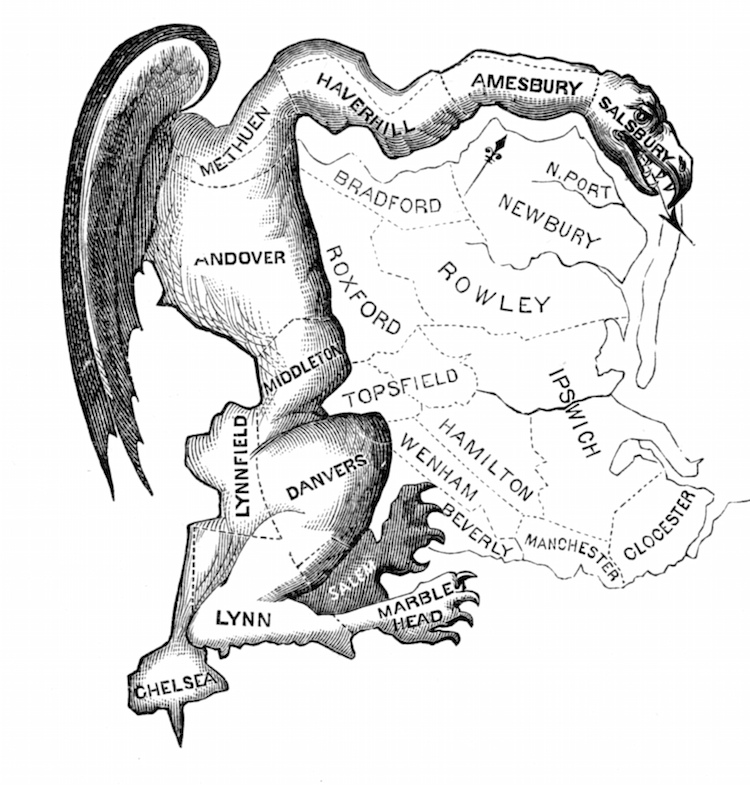
\includegraphics[width=.5\columnwidth]{gerrymander}%
\label{fig:gerrymander}%
%\end{figure}
%\end{wrapfigure}
\end{tabular}


Consider the simple state\footnote{Diagrams adapted from Stephen Nass, ``How to Steal an Election''}: 
\newcommand{\district}{
	%locations of participants
	\begin{scope}[shift = {(-.1, -.1)}]
			\draw[very thick] (0,0) -- (10,0) -- (10,5) -- (0,5) -- cycle;
	\end{scope}
	 \foreach \y in {0,1}
	 \foreach \x in {0,1,2,3,4,5,6,7,8,9}
    \draw[teal, opacity = .2, fill = teal] (\x,\y) rectangle (\x+.8,\y+.8);
	 \foreach \y in {2,3,4}
	 \foreach \x in {0,1,2,3,4,5,6,7,8,9}
    \draw[orange, fill=orange] (\x,\y) rectangle (\x+.8,\y+.8);
}

%\begin{wrapfigure}{l}{.5\columnwidth}
\begin{center}
	\begin{tikzpicture}[scale=.5]
	\district
\end{tikzpicture}
\end{center}
%\end{wrapfigure}

There are 50 people in this state who belong to two different political parties.  The census says that they should have 5 seats, so we need to divide up these people into 5 groups.  
\begin{enumerate}
	 \begin{tabular}{m{.45\textwidth}m{.45\textwidth}}
	 \item Consider the following districting of this state. Who would win with a majority of votes in each district?  Who has an advantage in the legislature?  Does it seem fair? Are the people in each district connected to each other?  Are the districts generally compact? &\newcommand{\districta}{\begin{scope}[shift = {(-.1,-.1)}]
		\draw[very thick] (0,0 ) -- (10, 0 );
		\draw[very thick] (0,1 ) -- (10, 1 );
		\draw[very thick] (0,2 ) -- (10, 2 );
		\draw[very thick] (0,3 ) -- (10, 3 );
		\draw[very thick] (0,4 ) -- (10, 4 );
		\end{scope}}
	
	\begin{tikzpicture}[scale=.5]
		\district 
		\begin{scope}[shift = {(-.1,-.1)}]
			\draw[very thick] (0,0 ) -- (10, 0 );
		\draw[very thick] (0,1 ) -- (10, 1 );
		\draw[very thick] (0,2 ) -- (10, 2 );
		\draw[very thick] (0,3 ) -- (10, 3 );
		\draw[very thick] (0,4 ) -- (10, 4 );
		\end{scope}
			\end{tikzpicture} 
	 
	\end{tabular}
	
	
	\vfill
	\clearpage
	 \begin{tabular}{m{.45\textwidth}m{.45\textwidth}}
	 \item Consider the following districting of this state. Who would win with a majority of votes in each district?  Who has an advantage in the legislature?  Does it seem fair? Are the people in each district connected to each other?  Are the districts generally compact? &
	\newcommand{\districtb}{	
	\begin{scope}[shift={(-.1,-.1)}]
					\foreach \x in {0,2,4,6,8}
	\draw[very thick] (\x,0) -- (\x, 5);

	\end{scope}
	}\begin{tikzpicture}[scale=.5]
	\district
	\districtb
	\end{tikzpicture}
	\end{tabular}
	 
	\vfill
 \begin{tabular}{m{.5\textwidth}m{.5\textwidth}}
	 \item Consider the following districting of this state. Who would win with a majority of votes in each district?  Who has an advantage in the legislature?  Does it seem fair? Are the people in each district connected to each other?  Are the districts generally compact? &
		\newcommand{\districtc}{
		\begin{scope}[shift = {(-.1, -.1)}]
				\draw[very thick] (0,0) -- (0,1) -- (1,1) -- (1,4) -- (3,4) -- (3,1) -- (4,1) -- (4,0);
				\draw[very thick] (3,4) -- (4,4) -- (4,2) -- (5, 2) -- (5,5);
				\draw[very thick] (5, 2) -- (6,2) -- (6,4) -- (9,4) -- (9, 1) -- (10, 1);
				\draw[very thick] (7,4) -- (7,1) -- (6,1) -- (6,0);
		\end{scope}
}

\begin{tikzpicture}[scale=.5]
\district
	\districtc	
	\end{tikzpicture} \end{tabular}
	 
	\vfill

	

The last diagram is an example of the `packing' and `cracking' that are illustrative of modern gerrymandering.
\begin{description}
	\item[packing] Putting a very large number of voters who all vote the same way in a single district.  In this case, the election is won by these voters, but by a very large margin.\index{gerrymander!packing}
	\item[cracking] Putting a slight majority of voters for one party in a single district.  In this case, the election is won by these voters by a slim margin.  There are a lot of minority voters in the district, but not enough to ever win an election.\index{gerrymander!cracking}
\end{description}
\clearpage

\item The state below has approximately 40\% orange (\tikz{\draw[fill=orange,orange]  circle(1ex);}) people and 60\% teal (\tikz{\draw[fill=teal,teal, opacity = .2]  circle(1ex);}) people (each color was selected randomly).  Divide the state into 10 districts in such a way so that in an election 40\% of the seats will be won by the orange people and 60\% by the teal people.

\newcommand{\firstexample}{	\begin{scope}[shift = {(-.9, -.9)}]
\draw[teal, fill = teal, opacity = 0.4] (1, 1) rectangle (1.8, 1.8);	\draw[orange, fill = orange] (1, 2) rectangle (1.8, 2.8);	\draw[orange, fill = orange] (1, 3) rectangle (1.8, 3.8);	\draw[orange, fill = orange] (1, 4) rectangle (1.8, 4.8);	\draw[teal, fill = teal, opacity = 0.4] (1, 5) rectangle (1.8, 5.8);	\draw[orange, fill = orange] (1, 6) rectangle (1.8, 6.8);	\draw[orange, fill = orange] (1, 7) rectangle (1.8, 7.8);	\draw[teal, fill = teal, opacity = 0.4] (1, 8) rectangle (1.8, 8.8);	\draw[orange, fill = orange] (1, 9) rectangle (1.8, 9.8);	\draw[orange, fill = orange] (1, 10) rectangle (1.8, 10.8);
\draw[teal, fill = teal, opacity = 0.4] (2, 1) rectangle (2.8, 1.8);	\draw[teal, fill = teal, opacity = 0.4] (2, 2) rectangle (2.8, 2.8);	\draw[teal, fill = teal, opacity = 0.4] (2, 3) rectangle (2.8, 3.8);	\draw[teal, fill = teal, opacity = 0.4] (2, 4) rectangle (2.8, 4.8);	\draw[teal, fill = teal, opacity = 0.4] (2, 5) rectangle (2.8, 5.8);	\draw[orange, fill = orange] (2, 6) rectangle (2.8, 6.8);	\draw[teal, fill = teal, opacity = 0.4] (2, 7) rectangle (2.8, 7.8);	\draw[orange, fill = orange] (2, 8) rectangle (2.8, 8.8);	\draw[teal, fill = teal, opacity = 0.4] (2, 9) rectangle (2.8, 9.8);	\draw[teal, fill = teal, opacity = 0.4] (2, 10) rectangle (2.8, 10.8);
\draw[teal, fill = teal, opacity = 0.4] (3, 1) rectangle (3.8, 1.8);	\draw[teal, fill = teal, opacity = 0.4] (3, 2) rectangle (3.8, 2.8);	\draw[teal, fill = teal, opacity = 0.4] (3, 3) rectangle (3.8, 3.8);	\draw[teal, fill = teal, opacity = 0.4] (3, 4) rectangle (3.8, 4.8);	\draw[teal, fill = teal, opacity = 0.4] (3, 5) rectangle (3.8, 5.8);	\draw[orange, fill = orange] (3, 6) rectangle (3.8, 6.8);	\draw[orange, fill = orange] (3, 7) rectangle (3.8, 7.8);	\draw[teal, fill = teal, opacity = 0.4] (3, 8) rectangle (3.8, 8.8);	\draw[teal, fill = teal, opacity = 0.4] (3, 9) rectangle (3.8, 9.8);	\draw[teal, fill = teal, opacity = 0.4] (3, 10) rectangle (3.8, 10.8);
\draw[orange, fill = orange] (4, 1) rectangle (4.8, 1.8);	\draw[teal, fill = teal, opacity = 0.4] (4, 2) rectangle (4.8, 2.8);	\draw[teal, fill = teal, opacity = 0.4] (4, 3) rectangle (4.8, 3.8);	\draw[teal, fill = teal, opacity = 0.4] (4, 4) rectangle (4.8, 4.8);	\draw[orange, fill = orange] (4, 5) rectangle (4.8, 5.8);	\draw[orange, fill = orange] (4, 6) rectangle (4.8, 6.8);	\draw[orange, fill = orange] (4, 7) rectangle (4.8, 7.8);	\draw[teal, fill = teal, opacity = 0.4] (4, 8) rectangle (4.8, 8.8);	\draw[teal, fill = teal, opacity = 0.4] (4, 9) rectangle (4.8, 9.8);	\draw[teal, fill = teal, opacity = 0.4] (4, 10) rectangle (4.8, 10.8);
\draw[teal, fill = teal, opacity = 0.4] (5, 1) rectangle (5.8, 1.8);	\draw[orange, fill = orange] (5, 2) rectangle (5.8, 2.8);	\draw[teal, fill = teal, opacity = 0.4] (5, 3) rectangle (5.8, 3.8);	\draw[teal, fill = teal, opacity = 0.4] (5, 4) rectangle (5.8, 4.8);	\draw[orange, fill = orange] (5, 5) rectangle (5.8, 5.8);	\draw[teal, fill = teal, opacity = 0.4] (5, 6) rectangle (5.8, 6.8);	\draw[teal, fill = teal, opacity = 0.4] (5, 7) rectangle (5.8, 7.8);	\draw[teal, fill = teal, opacity = 0.4] (5, 8) rectangle (5.8, 8.8);	\draw[teal, fill = teal, opacity = 0.4] (5, 9) rectangle (5.8, 9.8);	\draw[teal, fill = teal, opacity = 0.4] (5, 10) rectangle (5.8, 10.8);
\draw[orange, fill = orange] (6, 1) rectangle (6.8, 1.8);	\draw[teal, fill = teal, opacity = 0.4] (6, 2) rectangle (6.8, 2.8);	\draw[orange, fill = orange] (6, 3) rectangle (6.8, 3.8);	\draw[teal, fill = teal, opacity = 0.4] (6, 4) rectangle (6.8, 4.8);	\draw[orange, fill = orange] (6, 5) rectangle (6.8, 5.8);	\draw[teal, fill = teal, opacity = 0.4] (6, 6) rectangle (6.8, 6.8);	\draw[orange, fill = orange] (6, 7) rectangle (6.8, 7.8);	\draw[orange, fill = orange] (6, 8) rectangle (6.8, 8.8);	\draw[orange, fill = orange] (6, 9) rectangle (6.8, 9.8);	\draw[orange, fill = orange] (6, 10) rectangle (6.8, 10.8);
\draw[teal, fill = teal, opacity = 0.4] (7, 1) rectangle (7.8, 1.8);	\draw[teal, fill = teal, opacity = 0.4] (7, 2) rectangle (7.8, 2.8);	\draw[teal, fill = teal, opacity = 0.4] (7, 3) rectangle (7.8, 3.8);	\draw[teal, fill = teal, opacity = 0.4] (7, 4) rectangle (7.8, 4.8);	\draw[teal, fill = teal, opacity = 0.4] (7, 5) rectangle (7.8, 5.8);	\draw[teal, fill = teal, opacity = 0.4] (7, 6) rectangle (7.8, 6.8);	\draw[teal, fill = teal, opacity = 0.4] (7, 7) rectangle (7.8, 7.8);	\draw[orange, fill = orange] (7, 8) rectangle (7.8, 8.8);	\draw[orange, fill = orange] (7, 9) rectangle (7.8, 9.8);	\draw[teal, fill = teal, opacity = 0.4] (7, 10) rectangle (7.8, 10.8);
\draw[teal, fill = teal, opacity = 0.4] (8, 1) rectangle (8.8, 1.8);	\draw[orange, fill = orange] (8, 2) rectangle (8.8, 2.8);	\draw[teal, fill = teal, opacity = 0.4] (8, 3) rectangle (8.8, 3.8);	\draw[teal, fill = teal, opacity = 0.4] (8, 4) rectangle (8.8, 4.8);	\draw[teal, fill = teal, opacity = 0.4] (8, 5) rectangle (8.8, 5.8);	\draw[orange, fill = orange] (8, 6) rectangle (8.8, 6.8);	\draw[orange, fill = orange] (8, 7) rectangle (8.8, 7.8);	\draw[orange, fill = orange] (8, 8) rectangle (8.8, 8.8);	\draw[teal, fill = teal, opacity = 0.4] (8, 9) rectangle (8.8, 9.8);	\draw[orange, fill = orange] (8, 10) rectangle (8.8, 10.8);
\draw[teal, fill = teal, opacity = 0.4] (9, 1) rectangle (9.8, 1.8);	\draw[orange, fill = orange] (9, 2) rectangle (9.8, 2.8);	\draw[orange, fill = orange] (9, 3) rectangle (9.8, 3.8);	\draw[teal, fill = teal, opacity = 0.4] (9, 4) rectangle (9.8, 4.8);	\draw[orange, fill = orange] (9, 5) rectangle (9.8, 5.8);	\draw[orange, fill = orange] (9, 6) rectangle (9.8, 6.8);	\draw[teal, fill = teal, opacity = 0.4] (9, 7) rectangle (9.8, 7.8);	\draw[orange, fill = orange] (9, 8) rectangle (9.8, 8.8);	\draw[teal, fill = teal, opacity = 0.4] (9, 9) rectangle (9.8, 9.8);	\draw[teal, fill = teal, opacity = 0.4] (9, 10) rectangle (9.8, 10.8);
\draw[orange, fill = orange] (10, 1) rectangle (10.8, 1.8);	\draw[teal, fill = teal, opacity = 0.4] (10, 2) rectangle (10.8, 2.8);	\draw[teal, fill = teal, opacity = 0.4] (10, 3) rectangle (10.8, 3.8);	\draw[orange, fill = orange] (10, 4) rectangle (10.8, 4.8);	\draw[teal, fill = teal, opacity = 0.4] (10, 5) rectangle (10.8, 5.8);	\draw[teal, fill = teal, opacity = 0.4] (10, 6) rectangle (10.8, 6.8);	\draw[orange, fill = orange] (10, 7) rectangle (10.8, 7.8);	\draw[teal, fill = teal, opacity = 0.4] (10, 8) rectangle (10.8, 8.8);	\draw[teal, fill = teal, opacity = 0.4] (10, 9) rectangle (10.8, 9.8);	\draw[orange, fill = orange] (10, 10) rectangle (10.8, 10.8);

	\end{scope}
}
\begin{tikzpicture}[scale=.75]
	\firstexample
	\begin{scope}[]
		\draw[very thick] (0,0) -- (0,10) -- (10,10) -- (10,0) -- cycle;
	\end{scope}
\end{tikzpicture}
\vfill

\item Now, divide the same state in such a way so that 60\% of the seats will be won by the orange people.\\
\begin{tikzpicture}[scale = .75]
	\firstexample
	\begin{scope}[]
		\draw[very thick] (0,0) -- (0,10) -- (10,10) -- (10,0) -- cycle;
	\end{scope}
\end{tikzpicture}
\vfill

\end{enumerate}
%<*HWHEADER>
\clearpage
%%%%%%%%%%%%%%%%%%%%%%%%%%%%%%%%%%%%%%%%%%%%%%%%%%%%%%%%%%%%%%%%%%%%%%%%%%%%%%%%%%%%%%%%%%%%%%%%%%%%%%%%
\HOMEWORK
%</HWHEADER>

%<*HOMEWORK>


\begin{Renumerate}

  \item Consider the following map.  Put 5 districts on the map so that orange receives the most seats.
	\newcommand{\homeworkone}{
		\begin{scope}[shift = {(-.9,-.9)}]
			\draw[orange, fill = orange] (1, 1) rectangle (1.8, 1.8);	
			\draw[teal, fill = teal, opacity = 0.4] (1, 2) rectangle (1.8, 2.8);	
			\draw[teal, fill = teal, opacity = 0.4] (1, 3) rectangle (1.8, 3.8);	
			\draw[teal, fill = teal, opacity = 0.4] (1, 4) rectangle (1.8, 4.8);	
			\draw[orange, fill = orange] (1, 5) rectangle (1.8, 5.8);
			\draw[orange, fill = orange] (2, 1) rectangle (2.8, 1.8);	
			\draw[teal, fill = teal, opacity = 0.4] (2, 2) rectangle (2.8, 2.8);	
			\draw[teal, fill = teal, opacity = 0.4] (2, 3) rectangle (2.8, 3.8);	
			\draw[teal, fill = teal, opacity = 0.4] (2, 4) rectangle (2.8, 4.8);	
			\draw[teal, fill = teal, opacity = 0.4] (2, 5) rectangle (2.8, 5.8);
			\draw[teal, fill = teal, opacity = 0.4] (3, 1) rectangle (3.8, 1.8);	
			\draw[orange, fill = orange] (3, 2) rectangle (3.8, 2.8);	
			\draw[teal, fill = teal, opacity = 0.4] (3, 3) rectangle (3.8, 3.8);	
			\draw[teal, fill = teal, opacity = 0.4] (3, 4) rectangle (3.8, 4.8);	
			\draw[teal, fill = teal, opacity = 0.4] (3, 5) rectangle (3.8, 5.8);
			\draw[orange, fill = orange] (4, 1) rectangle (4.8, 1.8);	
			\draw[orange, fill = orange] (4, 2) rectangle (4.8, 2.8);	
			\draw[orange, fill = orange] (4, 3) rectangle (4.8, 3.8);	
			\draw[orange, fill = orange] (4, 4) rectangle (4.8, 4.8);	
			\draw[teal, fill = teal, opacity = 0.4] (4, 5) rectangle (4.8, 5.8);
			\draw[teal, fill = teal, opacity = 0.4] (5, 1) rectangle (5.8, 1.8);	
			\draw[teal, fill = teal, opacity = 0.4] (5, 2) rectangle (5.8, 2.8);	
			\draw[orange, fill = orange] (5, 3) rectangle (5.8, 3.8);	
			\draw[teal, fill = teal, opacity = 0.4] (5, 4) rectangle (5.8, 4.8);	
			\draw[orange, fill = orange] (5, 5) rectangle (5.8, 5.8);
	\end{scope}
}
	
\begin{center}
		\begin{tikzpicture}
		\homeworkone
		\begin{scope}
			\draw[very thick] (0,0) -- (0,5) -- (5,5) -- (5,0)  --cycle;
		\end{scope}
	\end{tikzpicture}

\end{center}	
	\item Put 5 districts on the map so that teal receives the most districts.
	
\begin{center}
			\begin{tikzpicture}
		\homeworkone
		
		\begin{scope}
			\draw[very thick] (0,0) -- (0,5) -- (5,5) -- (5,0)  --cycle;
		\end{scope}
	\end{tikzpicture}

\end{center}
\end{Renumerate} 

\ENDHOMEWORK

%%%%%%%%%%%%%%%%%%%%%%%%%%%%%%%%%%%%%%%%%%%%%%%%%%%%%%%%%%%%%%%%%%%%%%%%%%%%%%%%%%%%%%%%%%%%%

\clearpage

\section{Fairness}
The big question of the day is 
\begin{quote}
Justice Kennedy suggested, as he did in another redistricting case 13 years ago, that courts perhaps could be involved in placing limits on extremely partisan electoral maps.  13 years ago he wrote "If courts refuse to entertain any claims of partisan gerrymandering, the temptation to use partisan favoritism in districting in an unconstitutional manner will grow," 
\end{quote}

\subsection{Geometric Measures} \index{redistricting:geometric measures of fairness}
Although most states have a requirement that their districts be compact, there is no good definition for how compact a set of districts would be.  We will look at two different ways of measuring compactness.  To make measurement easier, we will be using our example districts from before.

\subsubsection{Area vs. Perimeter}
One way of measuring how compact a district is comes from dividing the area of the district by its perimeter squared and then multiplying by 16\footnote{You multiply by 16 because the Isoperimetric measure for a square is $\frac{1}{16}$ and we would like our ratio to be about 1.}.  In general, this type of calculation is known as an Isoperimetric measure. \index{redistricting!isoperimetric measure}
\begin{enumerate}
	\item Example:
\begin{center}
		\begin{tikzpicture}[scale=.5]
		begin{scope}
		 \draw[orange, fill=orange] (0,0) rectangle (.8,.8);
		\draw[orange, fill=orange] (0,1) rectangle (.8,1+.8);
		\draw[orange, fill=orange] (0,2) rectangle (.8,2+.8);
		\draw[teal, opacity = .2, fill=teal] (1,0) rectangle (1+.8, .8);
		\draw[teal, opacity = .2, fill=teal] (1,1) rectangle (1+.8, 1+.8);
			\begin{scope}[shift = {(-.1, -.1)}]
			\draw[very thick] (0,0) -- (2,0) -- (2,2) -- (1,2) -- (1, 3) -- (0,3) -- cycle;
			
			\node at (6,2) {Area = 5};
			\node at (6,1) {Perimeter = 10 };
			\node at (14,2) {Ratio $= \frac{16\cdot5}{10^2} = 0.8$};
			\end{scope}
	\end{tikzpicture}
\end{center}
 \textbf{Notes.}         \fillwithlines{\stretch{1}}

\clearpage
\begin{tikzpicture}[scale=.5]
	\begin{scope}
			\district 
			\begin{scope}[shift = {(-.1,-.1)}]
		\draw[very thick] (0,0 ) -- (10, 0 );
		\draw[very thick] (0,1 ) -- (10, 1 );
		\draw[very thick] (0,2 ) -- (10, 2 );
		\draw[very thick] (0,3 ) -- (10, 3 );
		\draw[very thick] (0,4 ) -- (10, 4 );
		\end{scope}
		\begin{scope}[shift = {(.4,.4)}]
			\node at (0,0) {\textbf{E}};
			\node at (0,1) {\textbf{D}};
			\node at (0,2) {\textbf{C}};
			\node at (0,3) {\textbf{B}};
			\node at (0,4) {\textbf{A}};
		\end{scope}
			
			\node at (5,-2) {\textbf{Redistricting Plan 1}};
	\end{scope}
	
	\begin{scope}[shift = {(4.5in,0)}]
		\district 
		\begin{scope}[shift={(-.1,-.1)}]
					\foreach \x in {0,2,4,6,8}
	\draw[very thick] (\x,0) -- (\x, 5);

	\end{scope}
	
		\begin{scope}[shift={(.4,.4)}]
			\node at (0,0) {\textbf{A}};
			\node at (2,0) {\textbf{B}};
			\node at (4,0) {\textbf{C}};
			\node at (6,0) {\textbf{D}};
			\node at (8,0) {\textbf{E}};
		\end{scope}
			
			\node at (5,-2) {\textbf{Redistricting Plan 2}};
	\end{scope}
	
	\begin{scope}[shift = {(9in,0)}]
	\district 
		\begin{scope}[shift = {(-.1, -.1)}]
				\draw[very thick] (0,0) -- (0,1) -- (1,1) -- (1,4) -- (3,4) -- (3,1) -- (4,1) -- (4,0);
				\draw[very thick] (3,4) -- (4,4) -- (4,2) -- (5, 2) -- (5,5);
				\draw[very thick] (5, 2) -- (6,2) -- (6,4) -- (9,4) -- (9, 1) -- (10, 1);
				\draw[very thick] (7,4) -- (7,1) -- (6,1) -- (6,0);
		\end{scope}
			\begin{scope}[shift = {(.4,.4)}]
				\node at (0,1) {\textbf{A}};
			\node at (0,0) {\textbf{B}};
			\node at (4,0) {\textbf{C}};
			\node at (5,2) {\textbf{D}};
			\node at (6,0) {\textbf{E}};
			\end{scope}
			
			\node at (5,-2) {\textbf{Redistricting Plan 3}};
	\end{scope}
\end{tikzpicture}

\item Calculate the area and perimeter of each district for each plan.  Fill in the table below.
\begin{center} \renewcommand{\arraystretch}{1.5}
	\begin{tabular}{|cc||cc||cc|} \hline
	Plan 1 & $16\frac{\text{Area}}{\text{Perimeter}^2}$ & Plan 2 & $16\frac{\text{Area}}{\text{Perimeter}^2}$ & Plan 3 & $16\frac{\text{Area}}{\text{Perimeter}^2}$\\\hline
	District A & & District A & &District A & \\\hline
	District B & & District B & &District B & \\\hline
	District C & & District C & &District C & \\\hline
	District D & & District D & &District D & \\\hline
	District E & & District E & &District E & \\\hline
	Average && Average && Average &\\\hline
	\end{tabular}
\end{center}

\item Does the calculation differentiate between the plans?  Does it show one plan as being ``better'' than the others?   
 \fillwithlines{\stretch{1}}

\subsubsection{Enclosing Square}
Another way of measuring how compact a district is comes from thinking of placing the district into the smallest square that contains the district.  Then you calculate the area of the district and its' enclosing square and divide the first by the second.  Generally, this type of calculation is known as a Reock measure. \index{redistricting!Reock measure}  For example:
\begin{center}
	\begin{tikzpicture}[scale=.5]
		\begin{scope}
		\draw[orange, fill=orange] (0,0) rectangle (.8,.8);
		\draw[orange, fill=orange] (0,1) rectangle (.8,1.8);
		\draw[orange, fill=orange] (0,2) rectangle (.8,2.8);
		\draw[teal, opacity = .2, fill=teal] (1,0) rectangle (1.8,.8);
		\draw[teal, opacity = .2, fill=teal] (1,1) rectangle (1.8,1.8);
			\begin{scope}[shift = {(-.1, -.1)}]
			\draw[very thick] (0,0) -- (2,0) -- (2,2) -- (1,2) -- (1, 3) -- (0,3) -- cycle;
			
			\node at (6,2) {Area = 5};
			\end{scope}
		\end{scope}
		%\node at (4in,3) {vs.};
		\node at (4in,0) {Ratio = $\frac{5}{9}=0.56$};
		\begin{scope}[shift = {(6in,0)}]
		\draw[orange, fill=orange] (0,0) rectangle (.8,.8);
		\draw[orange, fill=orange] (0,1) rectangle (.8,1.8);
		\draw[orange, fill=orange] (0,2) rectangle (.8,2.8);
		\draw[teal, opacity = .2, fill=teal] (1,0) rectangle (1.8,.8);
		\draw[teal, opacity = .2, fill=teal] (1,1) rectangle (1.8,1.8);
			\begin{scope}[shift = {(-.1, -.1)}]
			\draw[very thick] (0,0) -- (3,0) -- (3,3) -- (0,3) -- cycle;
			\node at (6,2) {Area = 9};
			
			\end{scope}
		\end{scope}
	\end{tikzpicture}
\end{center}

\item 
 \textbf{Notes.}         \fillwithlines{\stretch{1}}

\clearpage
\begin{tikzpicture}[scale=.5]
	\begin{scope}
			\district 
			\begin{scope}[shift = {(-.1,-.1)}]
		\draw[very thick] (0,0 ) -- (10, 0 );
		\draw[very thick] (0,1 ) -- (10, 1 );
		\draw[very thick] (0,2 ) -- (10, 2 );
		\draw[very thick] (0,3 ) -- (10, 3 );
		\draw[very thick] (0,4 ) -- (10, 4 );
		\end{scope}
		\begin{scope}[shift = {(.4,.4)}]
			\node at (0,0) {\textbf{E}};
			\node at (0,1) {\textbf{D}};
			\node at (0,2) {\textbf{C}};
			\node at (0,3) {\textbf{B}};
			\node at (0,4) {\textbf{A}};
		\end{scope}
			
			\node at (5,-2) {\textbf{Redistricting Plan 1}};
	\end{scope}
	
	\begin{scope}[shift = {(4.5in,0)}]
		\district 
		\begin{scope}[shift={(-.1,-.1)}]
					\foreach \x in {0,2,4,6,8}
	\draw[very thick] (\x,0) -- (\x, 5);

	\end{scope}
	
		\begin{scope}[shift={(.4,.4)}]
			\node at (0,0) {\textbf{A}};
			\node at (2,0) {\textbf{B}};
			\node at (4,0) {\textbf{C}};
			\node at (6,0) {\textbf{D}};
			\node at (8,0) {\textbf{E}};
		\end{scope}
			
			\node at (5,-2) {\textbf{Redistricting Plan 2}};
	\end{scope}
	
	\begin{scope}[shift = {(9in,0)}]
	\district 
		\begin{scope}[shift = {(-.1, -.1)}]
				\draw[very thick] (0,0) -- (0,1) -- (1,1) -- (1,4) -- (3,4) -- (3,1) -- (4,1) -- (4,0);
				\draw[very thick] (3,4) -- (4,4) -- (4,2) -- (5, 2) -- (5,5);
				\draw[very thick] (5, 2) -- (6,2) -- (6,4) -- (9,4) -- (9, 1) -- (10, 1);
				\draw[very thick] (7,4) -- (7,1) -- (6,1) -- (6,0);
		\end{scope}
			\begin{scope}[shift = {(.4,.4)}]
				\node at (0,1) {\textbf{A}};
			\node at (0,0) {\textbf{B}};
			\node at (4,0) {\textbf{C}};
			\node at (5,2) {\textbf{D}};
			\node at (6,0) {\textbf{E}};
			\end{scope}
			
			\node at (5,-2) {\textbf{Redistricting Plan 3}};
	\end{scope}
\end{tikzpicture}

\item Calculate the area and perimeter of each district for each plan.  Fill in the table below.
\begin{center} \renewcommand{\arraystretch}{1.5}
	\begin{tabular}{|cc||cc||cc|} \hline
	Plan 1 & $\frac{\text{Area District}}{\text{Area square}}$ & Plan 2 & $\frac{\text{Area District}}{\text{Area square}}$ & Plan 3 & $\frac{\text{Area District}}{\text{Area square}}$\\\hline
	District A & & District A & &District A & \\\hline
	District B & & District B & &District B & \\\hline
	District C & & District C & &District C & \\\hline
	District D & & District D & &District D & \\\hline
	District E & & District E & &District E & \\\hline
	Average && Average && Average &\\\hline
	\end{tabular}
\end{center}

\item Does the calculation differentiate between the plans?  Does it show one plan as being ``better'' than the others?   
 \fillwithlines{\stretch{1}}
\item If you were asked to chose which method better differentiates your notion of compact, which would you use and why?
\fillwithlines{\stretch{1}}

%<*HWHEADER>
\clearpage
%%%%%%%%%%%%%%%%%%%%%%%%%%%%%%%%%%%%%%%%%%%%%%%%%%%%%%%%%%%%%%%%%%%%%%%%%%%%%%%%%%%%%%%%%%%%%%%%%%%%%%%%
\HOMEWORK
%</HWHEADER>

%<*HOMEWORK>


\begin{Renumerate}

  \item Go back to the 5 districts you drew on the map (or draw new ones) so that orange receives the most seats. What is your average calculation for $\frac{16\text{area}}{\text{perimeter}^2}$?  What is your average calculation for $\frac{\text{area of district}}{\text{area of enclosing square}}$?
	\newcommand{\homeworkone}{\begin{scope}[shift = {(-.9,-.9)}]
\draw[orange, fill = orange] (1, 1) rectangle (1.8, 1.8);	\draw[teal, fill = teal, opacity = 0.4] (1, 2) rectangle (1.8, 2.8);	\draw[teal, fill = teal, opacity = 0.4] (1, 3) rectangle (1.8, 3.8);	\draw[teal, fill = teal, opacity = 0.4] (1, 4) rectangle (1.8, 4.8);	\draw[orange, fill = orange] (1, 5) rectangle (1.8, 5.8);
\draw[orange, fill = orange] (2, 1) rectangle (2.8, 1.8);	\draw[teal, fill = teal, opacity = 0.4] (2, 2) rectangle (2.8, 2.8);	\draw[teal, fill = teal, opacity = 0.4] (2, 3) rectangle (2.8, 3.8);	\draw[teal, fill = teal, opacity = 0.4] (2, 4) rectangle (2.8, 4.8);	\draw[teal, fill = teal, opacity = 0.4] (2, 5) rectangle (2.8, 5.8);
\draw[teal, fill = teal, opacity = 0.4] (3, 1) rectangle (3.8, 1.8);	\draw[orange, fill = orange] (3, 2) rectangle (3.8, 2.8);	\draw[teal, fill = teal, opacity = 0.4] (3, 3) rectangle (3.8, 3.8);	\draw[teal, fill = teal, opacity = 0.4] (3, 4) rectangle (3.8, 4.8);	\draw[teal, fill = teal, opacity = 0.4] (3, 5) rectangle (3.8, 5.8);
\draw[orange, fill = orange] (4, 1) rectangle (4.8, 1.8);	\draw[orange, fill = orange] (4, 2) rectangle (4.8, 2.8);	\draw[orange, fill = orange] (4, 3) rectangle (4.8, 3.8);	\draw[orange, fill = orange] (4, 4) rectangle (4.8, 4.8);	\draw[teal, fill = teal, opacity = 0.4] (4, 5) rectangle (4.8, 5.8);
\draw[teal, fill = teal, opacity = 0.4] (5, 1) rectangle (5.8, 1.8);	\draw[teal, fill = teal, opacity = 0.4] (5, 2) rectangle (5.8, 2.8);	\draw[orange, fill = orange] (5, 3) rectangle (5.8, 3.8);	\draw[teal, fill = teal, opacity = 0.4] (5, 4) rectangle (5.8, 4.8);	\draw[orange, fill = orange] (5, 5) rectangle (5.8, 5.8);
	\end{scope}}
	
\begin{center}
		\begin{tikzpicture}
		\homeworkone
		
		\begin{scope}
			\draw[very thick] (0,0) -- (0,5) -- (5,5) -- (5,0)  --cycle;
		\end{scope}
	\end{tikzpicture}

\end{center}	
	\item Go back to the 5 districts you drew on the map (or draw new ones) so that teal receives the most seats. What is your average calculation for $\frac{16\text{area}}{\text{perimeter}^2}$?  What is your average calculation for $\frac{\text{area of district}}{\text{area of enclosing square}}$?
	
\begin{center}
			\begin{tikzpicture}
		\homeworkone
		
		\begin{scope}
			\draw[very thick] (0,0) -- (0,5) -- (5,5) -- (5,0)  --cycle;
		\end{scope}
	\end{tikzpicture}

\end{center}

\item Does the average of $\frac{16\text{area}}{\text{perimeter}^2}$ demonstrate unfairness in either of your plans? \vfill

\item Does the average of $\frac{\text{area of enclosing square}}{\text{area of district}}$ demonstrate unfairness in either of your plans? \vfill

\end{Renumerate} 

\ENDHOMEWORK

%%%%%%%%%%%%%%%%%%%%%%%%%%%%%%%%%%%%%%%%%%%%%%%%%%%%%%%%%%%%%%%%%%%%%%%%%%%%%%%%%%%%%%%%%%%%%

\clearpage
\subsection{Arithmetic Measures}\index{redistricting!arithmetic measures of fairness}
Okay, so maybe just looking geometrically at how the districts are drawn is not a good way of testing how fair a redistricting is.  Maybe there is something about the election and where the people who live in the district are placed that would help us measure the fairness of the redistricting plan.
\subsubsection{Efficiency Gap} \index{redistricting!efficiency gap} \index{gerrymander!efficiency gap}
A state has been divided into 5 districts of 100 voters each.  Each district votes to elect a representative from one of two parties, $A$ or $B$.  In any election, many voters will end up feeling that voting was a waste of their time.  A voter could feel this way for two reasons:
\begin{itemize}
	\item Her party lost, so what was the point of showing up to vote?
	\item Her party won by a landslide, so what was the point of showing up to vote?
\end{itemize}
Corresponding to this, we will count:
\begin{itemize}
	\item All of the votes for party $A$ as wasted if party $A$ looses.
	\item All of the votes above 50\% for party $A$ as wasted if party $A$ wins.
\end{itemize}
\item Complete the following table (we will use $W_A$ as a short cut for the votes wasted by party $A$.):
\begin{center}
	\begin{tabular}{|c||c|c|p{2cm}||p{1.5cm}|p{1.5cm}||p{2cm}|p{2cm}|}\hline
	District & A votes & B votes & Winner & $W_A$ & $W_B$ & $W_A+W_B$ & $W_A-W_B$\\\hline\hline\ifsolns
	1 & 95 & 5 & A & 45 & 5 & 50 & 40\\ \hline 
2 & 40 & 60 & B & 40 & 10 & 50 & 30\\ \hline 
3 & 75 & 25 & A & 25 & 25 & 50 & 0\\ \hline 
4 & 45 & 55 & B & 45 & 5 & 50 & 40\\ \hline 
5 & 45 & 55 & B & 45 & 5 & 50 & 40\\ \hline \hline 
	TOTAL & 300 & 200 & $A$: 2 $B$:3   & 200 & 50 & 250 & 150\\\hline
		\else
	1 & 95 & 5 & $A$ & 45 & 5 & 50 & 40\\\hline
	2 & 40 & 60 &  &  &  &  & \\\hline
	3 & 75 & 25 &  &  &  &  & \\\hline
	4 & 45 & 55 &  &  &  &  & \\\hline
	5 & 45 & 55 &  &  &  &  & \\\hline \hline
	TOTAL & 300 & 200 & $A$: \hspace{.75cm} $B$:\hspace{.75cm}   &  &  &  & \\\hline\fi
	\end{tabular}
\end{center}
The \textbf{Efficiency Gap} is defined to be the fraction of the difference of wasted votes divided by the total number of votes: \index{Efficiency Gap}
\[ \text{EG} = \frac{W_A-W_B}{\text{Votes}} =\]
The $V$ in the denominator normalized EG, so that its magnitude does not depend on the population of the state.  The idea is that when EG is much larger than 0, the districting plan may be unfair to party $A$, because $A$ is wasting more votes.  When EG is much smaller than 0, then $B$ is wasting more votes, so the plan may be unfair to $B$.  We do have to be careful because if a candidate is running unopposed, the efficiency gap for that election is meaningless.  We can either throw out that district in our calculations or use data from other elections to estimate what the election would look like if the seat were contested.

\item Consider the following election

\begin{center}
	\begin{tabular}{|c||c|c|p{2cm}||p{1.5cm}|p{1.5cm}||p{2cm}|p{2cm}|}\hline
	District & A votes & B votes & Winner & $W_A$ & $W_B$ & $W_A+W_B$ & $W_A-W_B$\\\hline\hline\ifsolns
		1 & 81 & 19 & A & 31 & 19 & 50 & 12\\ \hline 
		2 & 45 & 55 & B & 45 & 5 & 50 & 40\\ \hline 
		3 & 80 & 20 & A & 30 & 20 & 50 & 10\\ \hline 
		4 & 49 & 51 & B & 49 & 1 & 50 & 48\\ \hline 
		5 & 45 & 55 & B & 45 & 5 & 50 & 40\\ \hline  \hline 
	TOTAL & 300 & 200 & $A$: 2 $B$:3   & 200 & 50 & 250 & 150\\\hline
		\else
		1 & 81 & 19 &  &  &  &  & \\ \hline 
		2 & 45 & 55 &  &  &  &  & \\ \hline 
		3 & 80 & 20 &  &  &  &  & \\ \hline 
		4 & 49 & 51 &  &  &  &  & \\ \hline 
		5 & 45 & 55 &  &  &  &  &  \\ \hline \hline
	TOTAL & 300 & 200 & $A$: \hspace{.75cm} $B$:\hspace{.75cm}   &  &  &  & \\\hline\fi
	\end{tabular}
\end{center}
Fill out the table.  

\noindent Which districts show signs of \textbf{packing}, that is putting all the voters of one party together so that, although they win the district, they have a lot of wasted votes.
 \fillwithlines{\stretch{1}}
\noindent Which districts show signs of \textbf{cracking}, that is putting just enough voters of the opposing party in the district so that they are confident of winning the election and therefore the first party has a lot of wasted votes?
 \fillwithlines{\stretch{1}}

%<*HWHEADER>
\clearpage
%%%%%%%%%%%%%%%%%%%%%%%%%%%%%%%%%%%%%%%%%%%%%%%%%%%%%%%%%%%%%%%%%%%%%%%%%%%%%%%%%%%%%%%%%%%%%%%%%%%%%%%%
\HOMEWORK
%</HWHEADER>

%<*HOMEWORK>


\begin{Renumerate}

  \item Go back to the 5 districts you drew on the map (or draw new ones) so that orange receives the most seats. Assuming that each square represents 100 voters, what is the efficiency gap for your plan?
	\newcommand{\homeworkone}{\begin{scope}[shift = {(-.9,-.9)}]
\draw[orange, fill = orange] (1, 1) rectangle (1.8, 1.8);	\draw[teal, fill = teal, opacity = 0.4] (1, 2) rectangle (1.8, 2.8);	\draw[teal, fill = teal, opacity = 0.4] (1, 3) rectangle (1.8, 3.8);	\draw[teal, fill = teal, opacity = 0.4] (1, 4) rectangle (1.8, 4.8);	\draw[orange, fill = orange] (1, 5) rectangle (1.8, 5.8);
\draw[orange, fill = orange] (2, 1) rectangle (2.8, 1.8);	\draw[teal, fill = teal, opacity = 0.4] (2, 2) rectangle (2.8, 2.8);	\draw[teal, fill = teal, opacity = 0.4] (2, 3) rectangle (2.8, 3.8);	\draw[teal, fill = teal, opacity = 0.4] (2, 4) rectangle (2.8, 4.8);	\draw[teal, fill = teal, opacity = 0.4] (2, 5) rectangle (2.8, 5.8);
\draw[teal, fill = teal, opacity = 0.4] (3, 1) rectangle (3.8, 1.8);	\draw[orange, fill = orange] (3, 2) rectangle (3.8, 2.8);	\draw[teal, fill = teal, opacity = 0.4] (3, 3) rectangle (3.8, 3.8);	\draw[teal, fill = teal, opacity = 0.4] (3, 4) rectangle (3.8, 4.8);	\draw[teal, fill = teal, opacity = 0.4] (3, 5) rectangle (3.8, 5.8);
\draw[orange, fill = orange] (4, 1) rectangle (4.8, 1.8);	\draw[orange, fill = orange] (4, 2) rectangle (4.8, 2.8);	\draw[orange, fill = orange] (4, 3) rectangle (4.8, 3.8);	\draw[orange, fill = orange] (4, 4) rectangle (4.8, 4.8);	\draw[teal, fill = teal, opacity = 0.4] (4, 5) rectangle (4.8, 5.8);
\draw[teal, fill = teal, opacity = 0.4] (5, 1) rectangle (5.8, 1.8);	\draw[teal, fill = teal, opacity = 0.4] (5, 2) rectangle (5.8, 2.8);	\draw[orange, fill = orange] (5, 3) rectangle (5.8, 3.8);	\draw[teal, fill = teal, opacity = 0.4] (5, 4) rectangle (5.8, 4.8);	\draw[orange, fill = orange] (5, 5) rectangle (5.8, 5.8);
	\end{scope}}
	
\begin{center}
		\begin{tikzpicture}[scale=.5]
		\homeworkone
		
		\begin{scope}
			\draw[very thick] (0,0) -- (0,5) -- (5,5) -- (5,0)  --cycle;
		\end{scope}
	\end{tikzpicture}
	
	\begin{tabular}{|c||c|c||p{1.5cm}|p{1.5cm}||p{2cm}|}\hline
	District & O votes & T votes & $W_O$ & $W_T$ & $W_O-W_T$\\\hline\hline
	1&&&&&\\\hline
2&&&&&\\\hline
3&&&&&\\\hline
4&&&&&\\\hline
5&&&&&\\\hline
  \hline 
TOTAL &  &  &   &  & \\\hline
	\end{tabular}

\end{center}	
	\item Go back to the 5 districts you drew on the map (or draw new ones) so that teal receives the most seats. Assuming that each square represents 100 voters, what is the efficiency gap for your plan?
	
\begin{center}
			\begin{tikzpicture}[scale=.5]
		\homeworkone
		
		\begin{scope}
			\draw[very thick] (0,0) -- (0,5) -- (5,5) -- (5,0)  --cycle;
		\end{scope}
	\end{tikzpicture}
	
		\begin{tabular}{|c||c|c||p{1.5cm}|p{1.5cm}||p{2cm}|}\hline
	District & O votes & T votes & $W_O$ & $W_T$ & $W_O-W_T$\\\hline\hline
	1&&&&&\\\hline
2&&&&&\\\hline
3&&&&&\\\hline
4&&&&&\\\hline
5&&&&&\\\hline
  \hline 
TOTAL &  &  &   &  & \\\hline
	\end{tabular}


\end{center}

\item Does the efficiency gap calculation demonstrate unfairness in either of your plans? \vfill
\end{Renumerate} 

\ENDHOMEWORK

%%%%%%%%%%%%%%%%%%%%%%%%%%%%%%%%%%%%%%%%%%%%%%%%%%%%%%%%%%%%%%%%%%%%%%%%%%%%%%%%%%%%%%%%%%%%%

\clearpage



%\subsection{Votes vs Seats}
\end{enumerate}

%\include{chapter-Statistics}
\include{chapter-Infinity}

\appendix
\chapter{Answers to Selected Exercises}

{\footnotesize
% \parindent 0.3cm
% \parskip 0cm
% %\topmargin 0.2cm
 \oddsidemargin 0in
 \evensidemargin -0.5in
 \textwidth 7.0in
 \linewidth 7.0in
 \hsize 7.0in
% \textheight 9in
  \columnsep 0.5in
  \solnstrue
  \studentsolnstrue
  \gradersolnsfalse

  \ifnum\arabic{numstudentsolns}>0\relax
    \setlength{\columnseprule}{0.4pt}
    \begin{multicols}{2}
      \begin{enumerate}
        \foreach \k in {1,...,\arabic{numstudentsolns}}
          {\item[\csname studentsoln-label-\romannumeral\k\endcsname.]
                \csname studentsoln-\romannumeral\k\endcsname
          }
      \end{enumerate}
    \end{multicols}
  \fi
\newpage
}

\def\calckey#1{\fbox{\raisebox{0pt}[6pt][0pt]{\footnotesize\tt #1}}}

\def\calcscreen#1{%
\begin{center}%
  \fbox{%
    \begin{minipage}{2in}
      \tt
      #1
    \end{minipage}
  }
\end{center}%
}
\def\ca{\rule{0pt}{0pt}\hfill}

\def\caret{\char`\^}

\def\rightkey{\calckey{$\blacktriangleright$}}
\def\stokey{\calckey{STO$\blacktriangleright$}}

\def\tineg{\raisebox{1pt}[0pt][0pt]{-}}

\def\sto{\ensuremath{\rightarrow}}

\chapter{Calculator Tips}

Chapter \ref{ch:finance} requires the use of a calculator to evaluate some rather complicated formulas.
This appendix contains some advice on how to avoid pitfalls that sometimes afflict students.
Most of the advice applies to all calculators, but some is geared specifically to Texas Instruments calculators
like the TI-84 and TI-30.

\section{Parentheses}

One of the greatest challenges to students is using parentheses correctly to help a calculator interpret a formula correctly.
For example, consider the expression
\[\frac{1+7}{2}.\]
We know from elementary school that you compute the whole numerator of the fraction before dividing by the denominator,
so this expression equals $4$.
If you type it into the calculator without parentheses, however, we get
\calcscreen{1+7/2 \\
            \ca 4.5}
That's because the calculator, following the order of operations we learned as children,
first does the division and then the addition: ${\tt 7/2} = 3.5$, so ${\tt 1+7/2}=4.5$.

We human beings can tell, by looking at $\frac{1+7}{2}$, that the $1+7$ has to be done first,
but the calculator doesn't know that unless we tell it.  So we should really type
\calcscreen{(1+7)/2 \\
            \ca 4}
One way to make this process easier, especially in long complicated formulas, is to draw in the extra parentheses on your paper before you begin typing into the calculator.
\[\mbox{Given~}\frac{1+7}{2},\mbox{~draw in~}\frac{\textcolor{red}{(}1+7\textcolor{red}{)}}{2}\mbox{~and then type~}{\tt (1+7)/2}.\]

Here are some locations that typically need extra parentheses:
\begin{itemize}
  \item The numerator of a fraction:
        \begin{center}
            $\dfrac{1+7}{2}$ becomes $\dfrac{\textcolor{red}{(}1+7\textcolor{red}{)}}{2}$. \\
          \begin{tabular}{ll}
            \textbf{Incorrect:} & \textbf{Correct:} \\
            \fbox{\begin{minipage}{2in} \tt
              1+7/2 \\
              \ca 4.5
            \end{minipage}}
            &              
            \fbox{\begin{minipage}{2in} \tt
              (1+7)/2 \\
              \ca 4
            \end{minipage}}
          \end{tabular}
        \end{center}
  \item The denominator of a fraction:
        \begin{center}
            $\dfrac{\quad8\quad}{\frac{6}{3}}$ becomes $\dfrac{\quad8\quad}{\textcolor{red}{(}\frac{6}{3}\textcolor{red}{)}}$. \\
          \begin{tabular}{ll}
            \textbf{Incorrect:} & \textbf{Correct:} \\
            \fbox{\begin{minipage}{2in} \tt
              8/6/3 \\
              \ca 0.444444
            \end{minipage}}
            &              
            \fbox{\begin{minipage}{2in} \tt
              8/(6/3) \\
              \ca 4
            \end{minipage}}
          \end{tabular}
        \end{center}
  \item Exponents:\footnote{Some more recent Texas Instrument calculators help you out by making exponents actually look like exponents.
                            On such a calculator, if you press the keys \calckey5\,\calckey{\caret}\,\calckey6\,\calckey{-}\,\calckey4\,, it will display as
                            \calcscreen{$\tt 5^{6-4}$ \\ \ca 25}
                            On this kind of calculator, if you need to type more \emph{after} the exponent, press the right arrow key \rightkey\ to get ``back down'' to the main line.
                            For example, to evaluate $5^{6-4}+7$ on such a calculator, you would press the buttons
                            \calckey5\,\calckey{\caret}\,\calckey6\,\calckey{-}\,\calckey4\,\rightkey\,\calckey{+}\,\calckey7
                            to get
                            \calcscreen{$\tt 5^{6-4}+7$ \\ \ca 32}}
        \begin{center}
            $5^{6-4}$ becomes $5^{\textcolor{red}{(}6-4\textcolor{red}{)}}$. \\
          \begin{tabular}{ll}
            \textbf{Incorrect:} & \textbf{Correct:} \\
            \fbox{\begin{minipage}{2in} \tt
              5\caret6-4 \\
              \ca 15621
            \end{minipage}}
            &              
            \fbox{\begin{minipage}{2in} \tt
              5\caret(6-4) \\
              \ca 25
            \end{minipage}}
          \end{tabular}
        \end{center}

        

\end{itemize}
Of course, one complicated expression may need all of these!
        \begin{center}
            $500\dfrac{\left(1+\frac{.07}{52}\right)^{8\cdot52}-1}{\frac{.07}{52}}$ becomes 
            $500\dfrac{\textcolor{red}{\Big(}\left(1+\frac{.07}{52}\right)^{\textcolor{red}{(}8\cdot52\textcolor{red}{)}}-1\textcolor{red}{\Big)}}{\textcolor{red}{(}\frac{.07}{52}\textcolor{red}{)}}$.  \\
          \begin{tabular}{ll}
            \textbf{Incorrect:} & \textbf{Correct:} \\
            \fbox{\begin{minipage}{2in} \tt
              500*(1+.07/52)\caret8*52-1/ \\
              .07/52 \\
              \ca 26281.04806
            \end{minipage}}
            &              
            \fbox{\begin{minipage}{2in} \tt
              500*((1+.07/52)\caret(8*52) \\
              -1)/(.07/52) \\
              \ca 278576.3860
            \end{minipage}}
          \end{tabular}
        \end{center}


\section{Rounding Errors}

We all know that $\frac{1}{3} \times 300 = 100$, 
but sometimes when working with a calculator we can get wrong answers:
\calcscreen{1/3 \\
            \ca .3333333333 \\
            .3333333333*300 \\
            \ca 99.99999999}
The calculator is not at fault here; it has not made any mistakes.
The decimal equivalent of $\rec{3}$ is $0.33333333333333333333\ldots$;
it goes on forever.  The calculator gives us as many digits as it can,
but {\tt .3333333333} is just a \emph{rounded-off approximation} of $\rec{3}$.
When we then typed {\tt .3333333333} back into the calculator and multiplied by 300,
the calculator accurately told us the answer was 99.99999999, not 100.
This is called an \emph{rounding error}.

In this example, the difference between what the calculator told us and the real answer
is only $0.00000001$, which is not terribly bad.
Often students round off long decimals to only a few decimal places,
which is okay for a final answer, but then they run into more problems:
\calcscreen{1/3 \\
            \ca .3333333333 \\
            .33*300 \\
            \ca 99}
Now we got an answer of 99 instead of 100, which seems more significant.
In the more complicated expressions of the financial math chapter,
we can end up with errors of several dollars (possibly hundreds of dollars) if we're not careful.
For example, if we need to calculate $\$600 \cdot \frac{1-(1+\frac{.07}{12})^{-12\cdot 25}}{\frac{.07}{12}}$,%$\ds \$600 \cdot \frac{1-(1+\frac{.07}{12})^{-12\cdot 25}}{\frac{.07}{12}}$,
a common student error would be this:
\calcscreen{(1-(1+.07/12)\caret(\tineg12*25))/\\
            (.07/12) \\
            \ca 141.486903386 \\
            600*141.49 \\
            \ca 84894}
Whereas this student answered \$84,894.00,
the correct answer (to the nearest penny) is \$84,892.14;
that's \$1.86 too high, enough to lose points on a test.

Thus when the calculator gives you numbers you will use again later in the problem,
\emph{never round them off}.  Always type back in \emph{all} the digits.
Only round off at the very end of the problem!

However, this can \emph{still} cause small errors (as we saw in the first example),
and it's annoying to punch {\tt 141.486903386} into the calculator.
There are at least three better solutions to the rounding error problem,
all of which involve \emph{keeping the numbers in the calculator until the end}.

\begin{itemize}
  \item One solution is to combine your whole formula into one step in the calculator.
        \begin{center}
          \begin{tabular}{ll}
            \textbf{Example 1:} & \textbf{Example 2:} \\
            \fbox{\begin{minipage}[t]{2in} \tt
              (1/3)*300 \\
              \ca 100
            \end{minipage}}
            &              
            \fbox{\begin{minipage}[t]{2in} \tt
              600*(1-(1+.07/12)\caret(\tineg12*\\
              25))/(.07/12) \\
              \ca 84892.1420313
            \end{minipage}}
          \end{tabular}
        \end{center}
        The downside of this approach is that 
        writing the formula all in one line can be long,
        error-prone, and just plain unpleasant.

  \item An alternative is to break up your calculation into steps using {\tt Ans}.
        Most calculators have a feature to remember the most recent answer
        they computed; on a TI machine, this is represented by the symbol {\tt Ans}.
        The {\tt Ans} automatically appears if you start a line by pressing an operation like \calckey{+} or \calckey{$\div$}\,,
        or you can also get it by pressing the \calckey{2ND} key 
        and then the \calckey{(-)} key.
        \begin{center}
          \begin{tabular}{ll}
            \textbf{Example 1:} & \textbf{Example 2:} \\
            \fbox{\begin{minipage}[t]{2in} \tt
              1/3 \\
              \ca 0.3333333333 \\
              Ans*300 \\
              \ca 100
            \end{minipage}}
            &              
            \fbox{\begin{minipage}[t]{2in} \tt
              (1-(1+.07/12)\caret(\tineg12*25))/\\
              (.07/12) \\
              \ca 141.486903386 \\
              600*Ans\\
              \ca 84892.1420313
            \end{minipage}}
          \end{tabular}
        \end{center}
        In Example 1, the keystrokes used were 
        \calckey1\,\calckey/\,\calckey3\,\calckey{ENTER}
        and then
        \calckey*\,\calckey3\,\calckey0\,\calckey0\,\calckey{ENTER}\,;
        the {\tt Ans} was automatically generated by the calculator.
        In Example 2, 
        the keys punched in the second line were
        \calckey6\,\calckey0\,\calckey0\,\calckey*\,\calckey{2ND}\,\calckey{(-)}\,\calckey{ENTER}\,.

  \item The calculator's {\tt Ans} ability remembers just one number,
        the result of the most recent calculation.
        There is also a more powerful way to use the calculator's memory,
        using \emph{variables}, which are letters that stand for numbers.

        Most keys on your TI calculator have a letter printed above them and to the right;
        on a TI-84 Plus Silver Edition calculator, for example, one key looks like this: \\
        \centerline{%
          \tt\begin{tabular}{c}
               \tiny TEST \hfill \footnotesize A \\
               \fbox{MATH}
             \end{tabular}}
        \medskip
        
        To get the letter, you first press the \calckey{ALPHA} key,
        and then the key with the desired letter;
        for example, \calckey{ALPHA}\,\calckey{MATH} produces an ``{\tt A}'' on the screen.

        You can make the calculator remember any number at all 
        by \emph{storing} it to a variable, whose name is a letter.
        You use the \stokey\ key, 
        which writes a little ``$\rightarrow$'' symbol on the screen.  
        Then you choose which letter you want to represent your number,
        and press \calckey{ENTER}.
        The first line of this example was created on my TI-84 Plus Silver Edition by pressing
        \calckey5\,\stokey\,\calckey{ALPHA}\,\calckey{A}\,\calckey{ENTER}\,.
        \calcscreen{4+1$\rightarrow$A \\
                    \ca 5 \\
                    5-2$\rightarrow$B \\
                    \ca 3 \\
                    A*B \\
                    \ca 15}
        The use of variables can be immensely helpful, 
        especially if you are doing lots of calculations with the same numbers;
        they also sometimes mean you need fewer parentheses.
        Take a look at our two examples one last time.
        \begin{center}
          \begin{tabular}{ll}
            \textbf{Example 1:} & \textbf{Example 2:} \\
            \fbox{\begin{minipage}[t]{2in} \tt
              1/3\sto F \\
              \ca 0.3333333333 \\
              F*300 \\
              \ca 100
            \end{minipage}}
            &              
            \fbox{\begin{minipage}[t]{2in} \tt
              .07/12\sto I \\
              \ca .005833333333 \\
              12*25\sto M \\
              \ca 300 \\
              (1-(1+I)\caret-M)/I\sto A \\
              \ca 141.486903386 \\
              600*A\\
              \ca 84892.1420313
            \end{minipage}}
          \end{tabular}
        \end{center}
\end{itemize}

\clearpage
\section{Subtraction versus Negatives}

On Texas Instruments calculators, there are two keys with horizontal lines.
The main \calckey{-} key is for \emph{subtraction}, like $5-4$.
When you type in a \emph{negative number} like $-6$, however, 
you must use the smaller \calckey{(-)} key, usually located in the bottom row
of your calculator.
If you use the wrong button, you will probably see a screen like this:
\calcscreen{ERR:SYNTAX \\
            \raisebox{-2pt}{\makebox[0pt][l]{\rule{12pt}{11pt}}}\textcolor{white}{1:}Quit \\
            2:Goto}

\section{Correcting Mistakes}

At some point in this course you will probably type in a long, complex expression wrong,
and you'll have to fix it.
Instead of retyping the whole thing, you might be able to just edit your earlier attempt!
One of the following may work on your calculator:
\begin{itemize}
  \item pressing the up arrow key \fbox{$\blacktriangle$} to scroll up to the earlier line
  \item pressing \fbox{\tt \footnotesize 2ND}\,\fbox{\footnotesize\tt ENTER} 
        to access the latest ``{\tt\footnotesize ENTRY}''
\end{itemize}
If you do this, you might need to insert new symbols, such as parentheses, into your earlier wrong entry.
Be sure to change into insert mode (``{\tt \footnotesize INS}'')
by pressing \fbox{\tt \footnotesize 2ND}\,\fbox{\tt\footnotesize DEL}\,;
this will let you insert new characters.
Unfortunately, the calculator will switch back to normal ``overtype'' mode as soon as you press an arrow key to move to another location,
so you'll need to press \fbox{\tt \footnotesize 2ND}\,\fbox{\tt\footnotesize DEL} again.

\clearpage
\addcontentsline{toc}{chapter}{Index}
\printindex
\end{document}
